\documentclass[twoside,11pt]{article}

% ? Specify used packages
\usepackage{graphicx}        %  Use this one for final production.
% \usepackage[draft]{graphicx} %  Use this one for drafting.
\usepackage{array}
\usepackage{fancyhdr}
\usepackage{multirow}
% ? End of specify used packages
\usepackage{longtable}
\usepackage{color}
\usepackage{enumitem}
\pagestyle{myheadings}

% -----------------------------------------------------------------------------

% ? Document identification
\newcommand{\stardoccategory}  {Starlink Cookbook}
\newcommand{\stardocinitials}  {SC}
\newcommand{\stardocsource}    {sc\stardocnumber}
\newcommand{\stardoccopyright} {Copyright \copyright\ 2014 Science and Technology Facilities Council}
\newcommand{\stardocnumber}    {21.2}
\newcommand{\stardocauthors}   {H.\ S.\ Thomas, M.\ J.\ Currie}
\newcommand{\stardocdate}      {11 June 2014}
\newcommand{\stardoctitle}     {The SCUBA-2 Data Reduction Cookbook}
\newcommand{\stardocversion}   {1.3}
\newcommand{\stardocmanual}    {\ }
\newcommand{\stardocabstract}  {

   This cookbook provides a short introduction to Starlink facilities,
   especially \textsc{Smurf}, the Sub-Millimetre User Reduction
   Facility, for reducing, displaying, and calibrating SCUBA-2 data.
   It describes some of the data artefacts present in SCUBA-2
   time-series and methods to mitigate them. In particular, this
   cookbook illustrates the various steps required to reduce the data;
   and gives an overview of the Dynamic Iterative Map-Maker, which
   carries out all of these steps using a single command controlled by
   a configuration file. Specialised configuration files are
   presented.}

% ? End of document identification

% -----------------------------------------------------------------------------

% +
%  Name:
%     sc.tex
%
%  Purpose:
%     Template for Starlink Cookbook (SC) documents.
%     Refer to SUN/199
%
%  Authors:
%     AJC: A.J.Chipperfield (Starlink, RAL)
%     BLY: M.J.Bly (Starlink, RAL)
%     PWD: Peter W. Draper (Starlink, Durham University)
%
%  History:
%     16-JUN-1997 (BLY):
%        Original, based on SUN/SG templates.
%     13-AUG-1998 (PWD):
%        Converted for use with LaTeX2HTML version 98.2 and
%        Star2HTML version 1.3.
%      1-FEB-2000 (AJC):
%        Add Copyright statement in LaTeX
%     {Add further history here}
%
% -

\newcommand{\stardocname}{\stardocinitials /\stardocnumber}
\markboth{\stardocname}{\stardocname}
\setlength{\textwidth}{160mm}
\setlength{\textheight}{230mm}
\setlength{\topmargin}{-2mm}
\setlength{\oddsidemargin}{0mm}
\setlength{\evensidemargin}{0mm}
\setlength{\parindent}{0mm}
\setlength{\parskip}{\medskipamount}
\setlength{\unitlength}{1mm}

% -----------------------------------------------------------------------------
%  Hypertext definitions.
%  ======================
%  These are used by the LaTeX2HTML translator in conjunction with star2html.

%  Comment.sty: version 2.0, 19 June 1992
%  Selectively in/exclude pieces of text.
%
%  Author
%    Victor Eijkhout                                      <eijkhout@cs.utk.edu>
%    Department of Computer Science
%    University Tennessee at Knoxville
%    104 Ayres Hall
%    Knoxville, TN 37996
%    USA

%  Do not remove the %begin{latexonly} and %end{latexonly} lines (used by
%  LaTeX2HTML to signify text it shouldn't process).
%begin{latexonly}
\makeatletter
\def\makeinnocent#1{\catcode`#1=12 }
\def\csarg#1#2{\expandafter#1\csname#2\endcsname}

\def\ThrowAwayComment#1{\begingroup
    \def\CurrentComment{#1}%
    \let\do\makeinnocent \dospecials
    \makeinnocent\^^L% and whatever other special cases
    \endlinechar`\^^M \catcode`\^^M=12 \xComment}
{\catcode`\^^M=12 \endlinechar=-1 %
 \gdef\xComment#1^^M{\def\test{#1}
      \csarg\ifx{PlainEnd\CurrentComment Test}\test
          \let\html@next\endgroup
      \else \csarg\ifx{LaLaEnd\CurrentComment Test}\test
            \edef\html@next{\endgroup\noexpand\end{\CurrentComment}}
      \else \let\html@next\xComment
      \fi \fi \html@next}
}
\makeatother

\def\includecomment
 #1{\expandafter\def\csname#1\endcsname{}%
    \expandafter\def\csname end#1\endcsname{}}
\def\excludecomment
 #1{\expandafter\def\csname#1\endcsname{\ThrowAwayComment{#1}}%
    {\escapechar=-1\relax
     \csarg\xdef{PlainEnd#1Test}{\string\\end#1}%
     \csarg\xdef{LaLaEnd#1Test}{\string\\end\string\{#1\string\}}%
    }}

%  Define environments that ignore their contents.
\excludecomment{comment}
\excludecomment{rawhtml}
\excludecomment{htmlonly}

%  Hypertext commands etc. This is a condensed version of the html.sty
%  file supplied with LaTeX2HTML by: Nikos Drakos <nikos@cbl.leeds.ac.uk> &
%  Jelle van Zeijl <jvzeijl@isou17.estec.esa.nl>. The LaTeX2HTML documentation
%  should be consulted about all commands (and the environments defined above)
%  except \xref and \xlabel which are Starlink specific.

\newcommand{\htmladdnormallinkfoot}[2]{#1\footnote{#2}}
\newcommand{\htmladdnormallink}[2]{#1}
\newcommand{\htmladdimg}[1]{}
\newcommand{\hyperref}[4]{#2\ref{#4}#3}
\newcommand{\htmlref}[2]{#1}
\newcommand{\htmlimage}[1]{}
\newcommand{\htmladdtonavigation}[1]{}

\newenvironment{latexonly}{}{}
\newcommand{\latex}[1]{#1}
\newcommand{\html}[1]{}
\newcommand{\latexhtml}[2]{#1}
\newcommand{\HTMLcode}[2][]{}

%  Starlink cross-references and labels.
\newcommand{\xref}[3]{#1}
\newcommand{\xlabel}[1]{}

%  LaTeX2HTML symbol.
\newcommand{\latextohtml}{\LaTeX2\texttt{HTML}}

%  Define command to re-centre underscore for Latex and leave as normal
%  for HTML (severe problems with \_ in tabbing environments and \_\_
%  generally otherwise).
\renewcommand{\_}{\texttt{\symbol{95}}}

% -----------------------------------------------------------------------------
%  Debugging.
%  =========
%  Remove % on the following to debug links in the HTML version using Latex.

% \newcommand{\hotlink}[2]{\fbox{\begin{tabular}[t]{@{}c@{}}#1\\\hline{\footnotesize #2}\end{tabular}}}
% \renewcommand{\htmladdnormallinkfoot}[2]{\hotlink{#1}{#2}}
% \renewcommand{\htmladdnormallink}[2]{\hotlink{#1}{#2}}
% \renewcommand{\hyperref}[4]{\hotlink{#1}{\S\ref{#4}}}
% \renewcommand{\htmlref}[2]{\hotlink{#1}{\S\ref{#2}}}
% \renewcommand{\xref}[3]{\hotlink{#1}{#2 -- #3}}
%end{latexonly}

% -----------------------------------------------------------------------------
% ? Document specific \newcommand or \newenvironment commands.

% Include special HTML versions of commands.

\newcommand{\eg}{{\it e.g.}}
\newcommand{\ie}{{\it i.e.}}

\newsavebox{\fmbox}
\newenvironment{fmpage}[1]{\begin{lrbox}{\fmbox}\begin{minipage}{#1}}{\end{minipage}\end{lrbox}\fbox{\usebox{\fmbox}}}

% A new environment for quoting verbatim
% Environment for indenting and using a small font.
\newenvironment{myquote}{\begin{quote}\begin{small}}{\end{small}\end{quote}}

\definecolor{gray}{RGB}{200,200,200}

% Shortcuts
% ---------

% Typographical shortcuts
\newcommand{\fcfbe}{$\mathrm{FCF_{beamequiv}}$}
\newcommand{\fcfb}{$\mathrm{FCF_{beam}}$}
\newcommand{\fcfa}{$\mathrm{FCF_{arcsec}}$}
\newcommand{\fcfm}{$\mathrm{FCF_{match}}$}

% SCUBA reference
%\newcommand{\scuba}{\htmladdnormallink{SCUBA}{http://www.jach.hawaii.edu/JCMT/}}

% Starlink Package names
\newcommand{\starlink}{\htmladdnormallink{Starlink}{http://starlink.jach.hawaii.edu}}

% Set up some common package names
\newcommand{\ccdpack}{\xref{\textsc{Ccdpack}}{sun139}{}}
\newcommand{\convert}{\xref{\textsc{Convert}}{sun55}{}}
\newcommand{\cupid}{\xref{\textsc{Cupid}}{sun255}{}}
\newcommand{\Figaro}{\xref{\textsc{Figaro}}{sun86}{}}
\newcommand{\fluxes}{\xref{\textsc{Fluxes}}{sun213}{}}
\newcommand{\gaia}{\xref{\textsc{Gaia}}{sun214}{}}
\newcommand{\Kappa}{\xref{\textsc{Kappa}}{sun95}{}}
\newcommand{\agi}{\xref{AGI}{sun48}{}}
\newcommand{\ndf}{\xref{NDF}{sun33}{}}
\newcommand{\surf}{\xref{\textsc{Surf}}{sun216}{}}
\newcommand{\jcmtdr}{\xref{\textsc{JCMTdr}}{sun132}{}}
\newcommand{\oracdr}{\htmladdnormallink{\textsc{Orac-dr}}{http://www.oracdr.org/oracdr}}
\newcommand{\photom}{\xref{\textsc{Photom}}{sun45}{}}
\newcommand{\picard}{\xref{\textsc{Picard}}{sun265}{}}
\newcommand{\smurf}{\xref{\textsc{Smurf}}{sun258}{}}
\newcommand{\ssds}{\xref{\textsc{Starlink Standard Data Structures}}{sgp38}{}}
\newcommand{\topcat}{\htmladdnormallink{\textsc{Topcat}}{http://www.starlink.ac.uk/topcat}}

% DR recipe names
\newcommand{\drrecipe}[1]{\texttt{#1}}

% Application tasks
\newcommand{\task}[1]{\textsf{#1}}

% ADAM parameters
\newcommand{\param}[1]{\texttt{#1}}

% GAIA menu functions and buttons.  Would like a bold texttt to mimic
% their appearance in GAIA, but the founts are not in regular LaTeX.
\newcommand{\gaiathing}[1]{\textbf{#1}}

% SMURF tasks
\newcommand{\calcnoise}{\xref{\task{calcnoise}}{sun258}{CALCNOISE}}
\newcommand{\clean}{\xref{\task{sc2clean}}{sun258}{SC2CLEAN}}
\newcommand{\concat}{\xref{\task{sc2concat}}{sun258}{SC2CONCAT}}
\newcommand{\configmeld}{\xref{\task{configmeld}}{sun258}{CONFIGMELD}}
\newcommand{\flatfield}{\xref{\task{flatfield}}{sun258}{FLATFIELD}}
\newcommand{\jcmtstate}{\xref{\task{jcmtstate2cat}}{sun258}{JCMTSTATE2CAT}}
\newcommand{\makemap}{\xref{\task{makemap}}{sun258}{MAKEMAP}}
\newcommand{\skyloop}{\xref{\task{skyloop}}{sun258}{SKYLOOP}}
\newcommand{\stackframes}{\xref{\task{stackframes}}{sun258}{STACKFRAMES}}

% KAPPA
\newcommand{\beamfit}{\xref{\task{beamfit}}{sun95}{BEAMFIT}}
\newcommand{\cmult}{\xref{\task{cmult}}{sun95}{CMULT}}
\newcommand{\compave}{\xref{\task{compave}}{sun95}{COMPAVE}}
\newcommand{\configecho}{\xref{\task{configecho}}{sun95}{CONFIGECHO}}
\newcommand{\fitslist}{\xref{\task{fitslist}}{sun95}{FITSLIST}}
\newcommand{\fitsval}{\xref{\task{fitsval}}{sun95}{FITSVAL}}
\newcommand{\hislist}{\xref{\task{hislist}}{sun95}{HISLIST}}
\newcommand{\histat}{\xref{\task{histat}}{sun95}{HISTAT}}
\newcommand{\histogram}{\xref{\task{histogram}}{sun95}{HISTOGRAM}}
\newcommand{\makesnr}{\xref{\task{makesnr}}{sun95}{MAKESNR}}
\newcommand{\ndfcopy}{\xref{\task{ndfcopy}}{sun95}{NDFCOPY}}
\newcommand{\ndftrace}{\xref{\task{ndftrace}}{sun95}{NDFTRACE}}
\newcommand{\provshow}{\xref{\task{provshow}}{sun95}{PROVSHOW}}
\newcommand{\showqual}{\xref{\task{showqual}}{sun95}{SHOWQUAL}}
\newcommand{\stats}{\xref{\task{stats}}{sun95}{STATS}}
\newcommand{\sub}{\xref{\task{sub}}{sun95}{SUB}}
\newcommand{\wcsmosaic}{\xref{\task{wcsmosaic}}{sun95}{WCSMOSAIC}}

% CCDPACK
\newcommand{\makemos}{\xref{\task{makemos}}{sun139}{MAKEMOS}}

% CUPID
\newcommand{\findback}{\xref{\task{findback}}{sun255}{FINDBACK}}
\newcommand{\findclumps}{\xref{\task{findclumps}}{sun255}{FINDCLUMPS}}

% Misc
\newcommand{\autophotom}{\xref{\task{autophotom}}{sun45}{AUTOPHOTOM}}

% Documents
\newcommand{\gaiasun}{\xref{\textbf{SUN/214}}{sun214}{}}
\newcommand{\kappasun}{\xref{\textbf{SUN/95}}{sun95}{}}
\newcommand{\picardsun}{\xref{\textbf{SUN/265}}{sun265}{}}
\newcommand{\pipelinesun}{\xref{\textbf{SUN/264}}{sun264}{}}
\newcommand{\smurfsun}{\xref{\textbf{SUN/258}}{sun258}{}}

% JAC
\newcommand{\Coulson}{\htmladdnormallink{Coulson}{http://www.jach.hawaii.edu/JACdocs/JCMT/SCD/SN/003/ }}

% Chapter title in the header. This is using package fancyhdr.
\pagestyle{fancy}
\renewcommand{\sectionmark}[1]{\markboth{\stardocname---#1}{\stardocname---#1}}
\renewcommand{\subsectionmark}[1]{}
\renewcommand{\headrulewidth}{0pt}
\lhead{\thepage}
\fancyfoot[c]{}
\fancyfoot[r]{}

% Figure environment. Defined for latex2html to produce good quality
% graphics in the hypertext. It assumes that the files are
% encapsulated PostScript with extension .eps, and PNG with extension
% .png. The arguments are: #1 graphics filename without an extension;
% #2 figure environment location including brackets, or leave empty for
% none; #3 the includegraphics % qualifiers; #4 the label; #5 is the
% short caption for the index of figures; and #6 is the full caption.
\newcommand{\myfig}[6]{
  \begin{figure}#2
    \centering\includegraphics[#3]{#1}
    \typeout{#1 inserted on page \arabic{page}}
    \caption[#5]{\label{#4}\small #6}
  \end{figure}
}
\begin{htmlonly}
  \newcommand{\myfig}[6]{
    \label{#4} \htmladdimg{#1.png}\\
    \\
    Figure: #6\\
  }
\end{htmlonly}

% Address twin (side-by-side) graphics in a similar fashion where the
% second argument is the second graphic, and the remaining arguments
% incremented by one slot save an extra argument #6 for the size of
% the gap between the two graphics, thus #7 and #8 are the captions.
\newcommand{\myfigduo}[8]{
  \begin{figure}#3
    \includegraphics[#4]{#1}
    \typeout{#1 inserted on page \arabic{page}}
    \hspace{#6}
    \includegraphics[#4]{#2}
    \typeout{#2 inserted on page \arabic{page}}
    \caption[#7]{\label{#5}\small #8}
  \end{figure}
}
\begin{htmlonly}
  \newcommand{\myfigduo}[8]{
    \label{#5} \htmladdimg{#1.png}\htmladdimg{#2.png}\\
    \\
    Figure: #8\\
  }
\end{htmlonly}

% A command to cross-reference in both LaTeX and hypertext.
% #1 is the type such as Section, Table, Figure; #2 is
% the label; and #3 is the text or title associated with the
% reference.
\newcommand{\cref}[3]{\latexhtml{#1~\ref{#2}}{\htmlref{#3}{#2}}}

% ? End of document specific commands
% -----------------------------------------------------------------------------
%  Title Page
%  ==========
\renewcommand{\thepage}{\roman{page}}
\begin{document}
\thispagestyle{empty}

%  Latex document header
%  =====================
\begin{latexonly}
   \textsc{Joint Astronomy Centre} \hfill \textbf{\stardocname}\\
   {\large Science \& Technology Facilities Council}\\
   {\large Starlink Project\\}
   {\large \stardoccategory\ \stardocnumber}
   \begin{flushright}
   \stardocauthors\\
   \stardocdate
   \end{flushright}
   \vspace{-4mm}
   \rule{\textwidth}{0.5mm}
   \vspace{5mm}
   \begin{center}
   {\Huge\textbf{\stardoctitle \\ [2.5ex]}}
   {\LARGE\textbf{\stardocversion \\ [4ex]}}
   {\Huge\textbf{\stardocmanual}}
   \end{center}
   \vspace{5mm}

% ? Add picture here if required for the LaTeX version.
%   e.g. \includegraphics[scale=0.3]{filename.ps}
% ? End of picture
   \begin{center}
   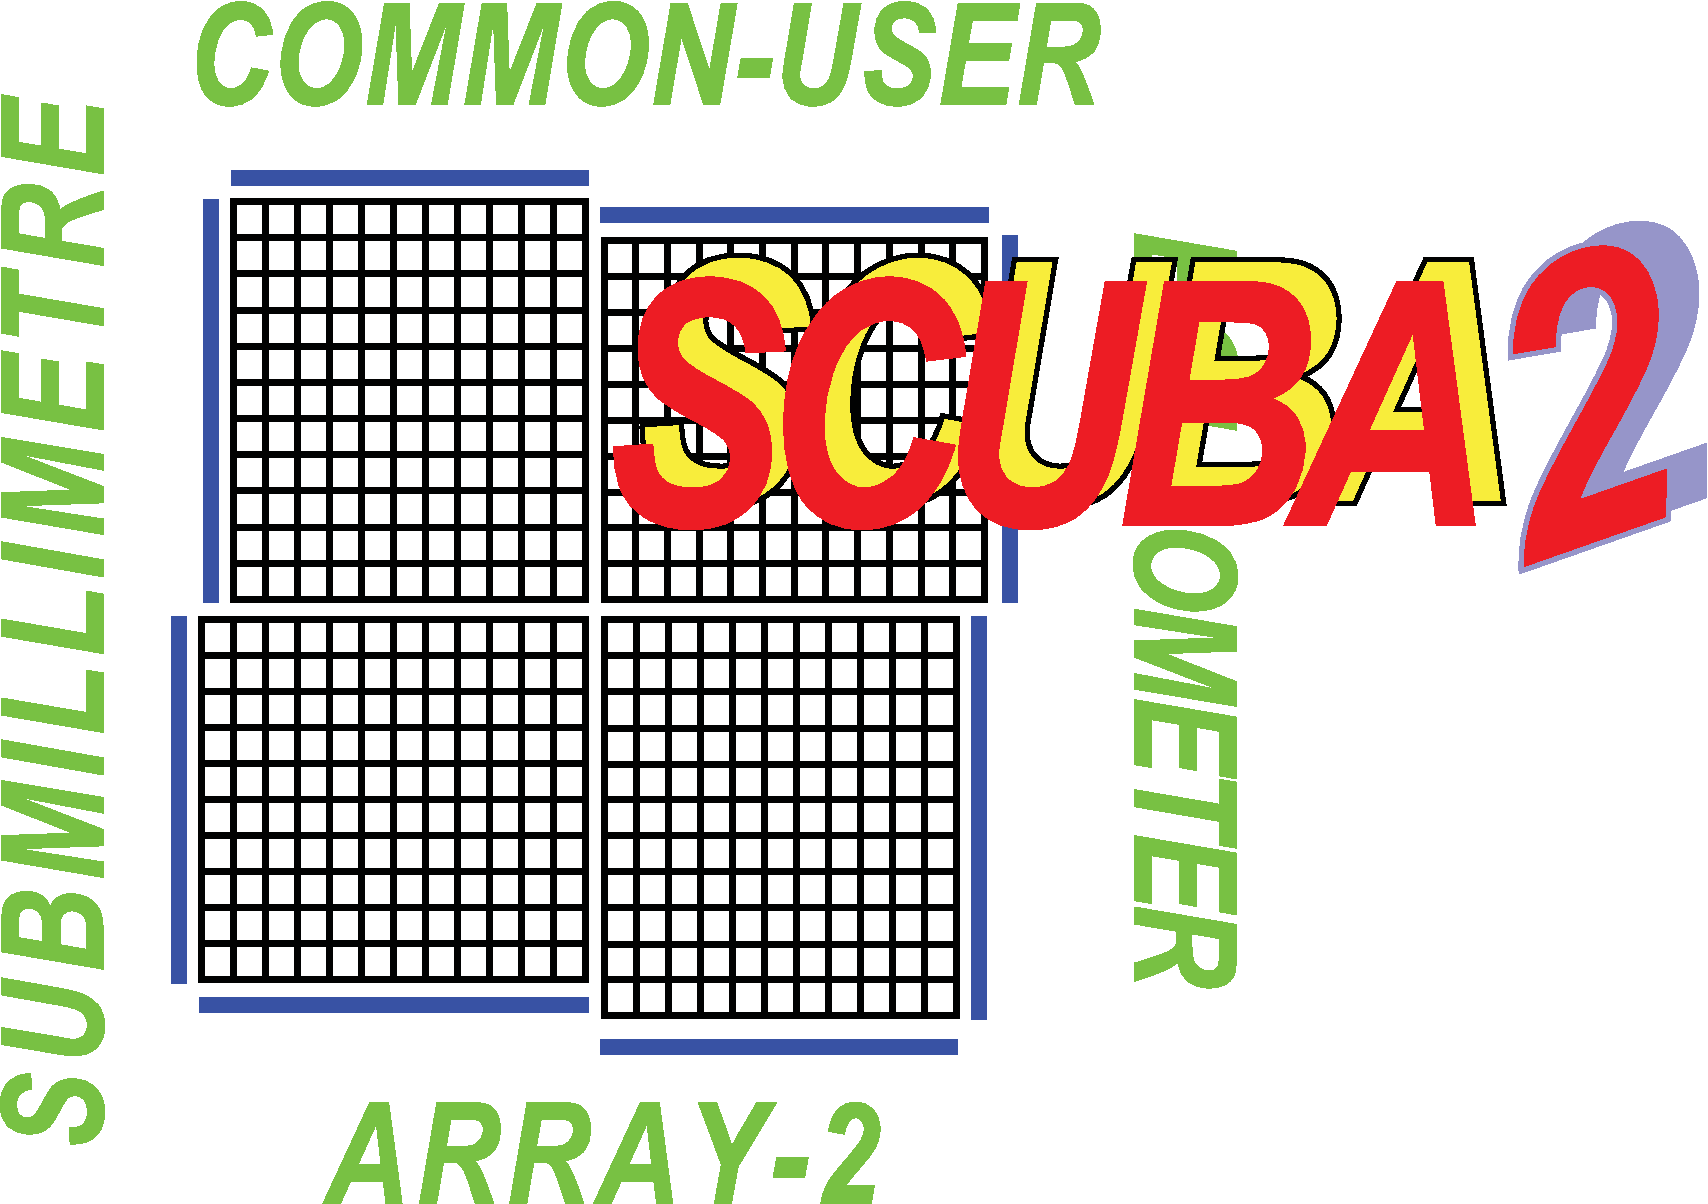
\includegraphics[scale=0.4]{sc21_s2logo}
   \end{center}
   \vspace{5mm}
   \rule{\textwidth}{0.5mm}\\
   \vspace{15mm}

% ? Heading for abstract if used.
   \vspace{10mm}
   \begin{center}
      {\Large\textbf{Abstract}}
   \end{center}
% ? End of heading for abstract.

\end{latexonly}

%  HTML documentation header
%  =========================
\begin{htmlonly}
   \xlabel{}
   \begin{rawhtml} <H1> \end{rawhtml}
      \stardoctitle\\
      \stardocversion\\
      \stardocmanual
   \begin{rawhtml} </H1> <HR> \end{rawhtml}

% ? Add picture here if required for the hypertext version.
%   e.g. \includegraphics[scale=0.5]{filename.ps}
   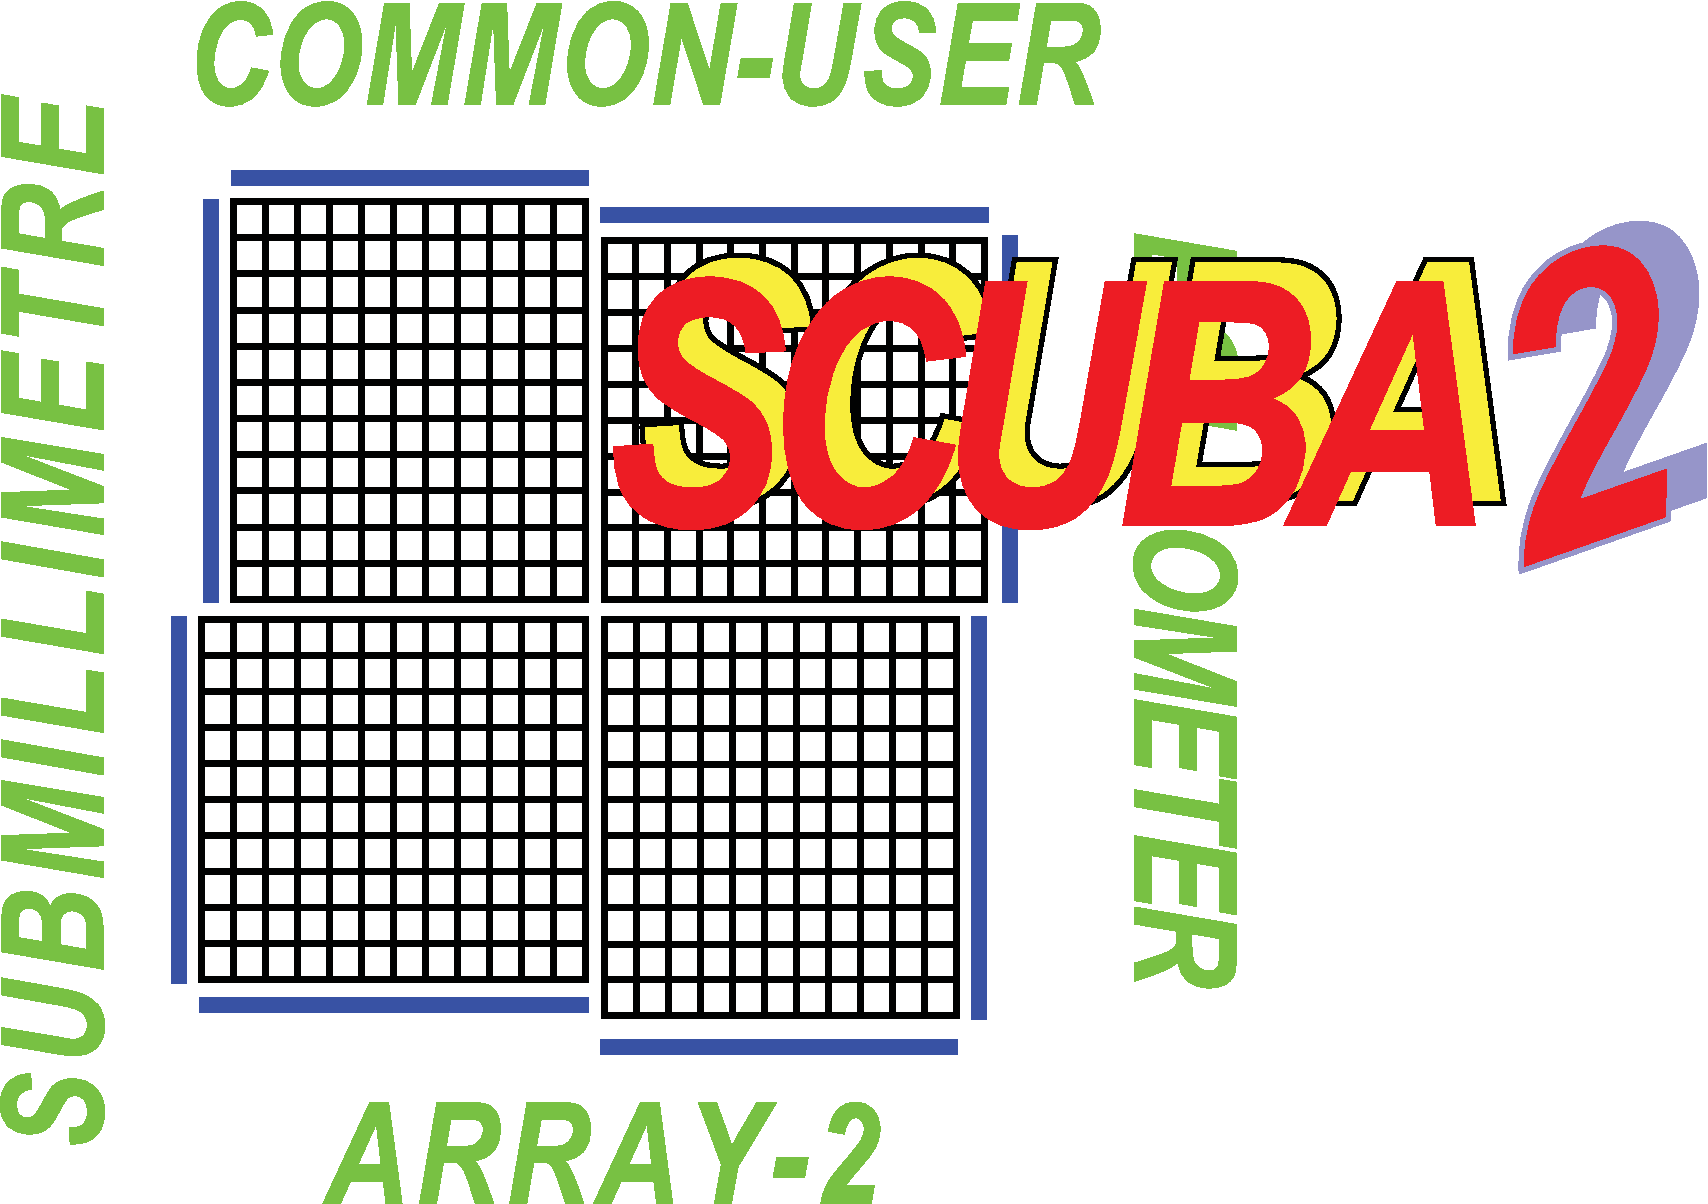
\includegraphics[width=90mm]{sc21_s2logo}
% ? End of picture

   \begin{rawhtml} <P> <I> \end{rawhtml}
   \stardoccategory\ \stardocnumber \\
   \stardocauthors \\
   \stardocdate
   \begin{rawhtml} </I> </P> <H3> \end{rawhtml}
      \htmladdnormallink{Joint Astronomy Centre}
                        {http://www.jach.hawaii.edu}\\
      \htmladdnormallink{Science \& Technology Facilities Council}
                        {http://www.scitech.ac.uk} \\
   \begin{rawhtml} </H3> <H2> \end{rawhtml}
      \htmladdnormallink{Starlink Project}{http://www.starlink.ac.uk/}
   \begin{rawhtml} </H2> \end{rawhtml}
   \htmladdnormallink{\htmladdimg{source.gif} Retrieve hardcopy}
      {http://www.starlink.ac.uk/cgi-bin/hcserver?\stardocsource}\\

%  HTML document table of contents
%  ===============================
%  Add table of contents header and a navigation button to return to this
%  point in the document (this should always go before the abstract \section).
  \label{stardoccontents}
  \begin{rawhtml}
    <HR>
    <H2>Contents</H2>
  \end{rawhtml}
  \htmladdtonavigation{\htmlref{\htmladdimg{contents_motif.gif}}
        {stardoccontents}}

% ? New section for abstract if used.
  \section{\xlabel{abstract}Abstract}
% ? End of new section for abstract
\end{htmlonly}

% -----------------------------------------------------------------------------
%  Document Abstract
%  =================
\stardocabstract
% ? End of document abstract

% -----------------------------------------------------------------------------
%  Latex Copyright Statement
%  =========================
\begin{latexonly}
  \newpage
  \vspace*{\fill}
  \stardoccopyright
\end{latexonly}
% ? End of Latex copyright statement

% -----------------------------------------------------------------------------
%  Latex document Table of Contents
%  ================================
  \newpage
  \begin{latexonly}
    \setlength{\parskip}{0mm}
    \tableofcontents
    \newpage
    \listoffigures
    \setlength{\parskip}{\medskipamount}
    \markboth{\stardocname}{\stardocname}
  \end{latexonly}
% ? End of Latex document table of contents

% -----------------------------------------------------------------------------

%  Glossary
%  ========
\newpage
\begin{latexonly}
\addcontentsline{toc}{section}{Acronyms}

% ? Heading for glossary if used.
   \vspace{10mm}
   \begin{center}
      {\Large\textbf{Acronyms}}
   \end{center}
% ? End of heading for glossary.

\setlength{\extrarowheight}{3pt}
\begin{table}[h!]
\begin{tabular}{ll}
\textbf{CADC}   & Canadian Astronomy Data Centre\\
\textbf{CSO}    & Caltech Submillimetre Observatory\\
\textbf{DIMM}   & Dynamic Iterative Map-Maker\\
\textbf{FCF}    & Flux Conversion Factor\\
\textbf{FITS}   & Flexible Image Transport System\\
\textbf{FWHM}   & Full-Width at Half-Maximum\\
\textbf{GAIA}   & Graphical Astronomy and Image Analysis Tool\\
\textbf{JCMT}   & James Clerk Maxwell Telescope\\
\textbf{NDF}    & Extensible N-Dimensional Data Format\\
\textbf{NEFD}   & Noise Equivalent Flux Density\\
\textbf{PSF}    & Point Spread Function\\
\textbf{SCUBA-2}& Submillimetre Common User Bolometer Array-2\\
\textbf{SMURF}  & Sub-Millimetre User Reduction Facility\\
\textbf{S/N}    & Signal-to-Noise ratio\\
\textbf{SQUID}  & Superconducting QUantum Interference Device\\
\textbf{SUN}    & Starlink User Note\\
\textbf{TES}    & Transition Edge Sensor\\
\textbf{WVM}    & Water Vapour radioMeter\\
\end{tabular}
\end{table}

\end{latexonly}

% -----------------------------------------------------------------------------

\cleardoublepage
\renewcommand{\thepage}{\arabic{page}}
\setcounter{page}{1}

\section{\xlabel{introduction}Introduction}
\label{sec:intro}

\subsection{\xlabel{using_guide}This Cookbook}


This guide is designed to instruct SCUBA-2 users on the best ways to
reduce and visualise their data using \starlink\ packages:
\smurf \cite{smurf}, \Kappa \cite{kappa}, \gaia \cite{gaia} and \picard
\cite{picard}.

This guide is not aimed at users of the
polarimeter (POL-2) or Fourier transform spectrometer (FTS-2). If you
have shared risk data (SRO) you should refer to the
\xref{SMURF SRO
Cookbook.}{sc19}{}\latex{\footnote{\texttt{http://www.starlink.ac.uk/docs/sc19.htx/sc19.html}}}


This guide covers the following:
\begin{itemize}
\itemsep0em
\item \cref{Chapter}{sec:intro}{Chapter 1} -- Computer resources you'll need before getting started.
\item \cref{Chapter}{sec:s2}{Chapter 2} -- A description of SCUBA-2 and its observing modes.
\item \cref{Chapter}{sec:raw}{Chapter 3}  -- Data acquisition and instructions for examining raw data.
\item \cref{Chapter}{sec:dimm}{Chapter 4}  -- An introduction to the Dynamic Iterative Map-Maker and a description of the available configuration files.
\item \cref{Chapter}{sec:maps}{Chapter 5}  -- Procedures for reducing your data using the map-maker.
\item \cref{Chapter}{sec:postprocess}{Chapter 6}  -- Post-processing reduction steps such as applying the FCF, co-adding multiple maps and estimating the noise.
\item \cref{Chapter}{sec:tweak}{Chapter 7}  -- Options for tailoring the configuration parameters to improve your final map.
\item \cref{Chapter}{sec:eg}{Chapter 8}  -- Two worked examples covering a \htmlref{blank cosmology field}{sec:cosmology} and a \htmlref{galactic field}{sec:bright_ex}.
\item \cref{Chapter}{sec:pipe}{Chapter 9}  -- Instructions for using the ORAC-DR pipeline to reduce your data along with details on data retrieved from the JSA.
\end{itemize}

\subsection{\xlabel{computing}Before you start: Computing resources}

Before reducing SCUBA-2 data using the Dynamic Iterative Map-Maker, we
recommend you confirm your resources are sufficient for your type of
map.

We recommend the following:\\
\begin{table}[h!]
\centering
\begin{tabular}{ll}
\hline
\textbf{Reduction type} &\textbf{Memory} \\
\hline
Large maps (\textsc{pong})& 96 GB\\
Small maps (\textsc{daisy})&32 - 64 GB\\
850\,$\mu$m data only&32 - 64 GB\\
Blank fields&32 - 64 GB\\
\hline
\end{tabular}
\end{table}

\textbf{Why these recommendations?}\\*
For large-area maps it is important to process a full observation in a
single chunk---see the text box on
\latexhtml{Page~\pageref{page:text}}{\htmlref{What to look
for}{box:chunk}} for an explanation of chunking. For large maps, using normal
map-maker parameters a machine of 96\,GB is acceptable. It is
important that the memory is as fast as can be afforded as RAM speed
has a direct linear effect on processing time given that the
time-series data are continually being funnelled through the CPU.

For blank field surveys, data that only use 850\,$\mu$m, or smaller
regions of the sky you can usefully run the map-maker with less memory
and 32 to 64\,GB is reasonable depending on the specifics of your data
set. SMURF is multi-threaded so multiple cores do help although above
8 cores the price/performance gains tend to drop off.

If you have a very large machine (128\,GB and 24 cores) you can to run
two instances of the map-maker in parallel. Use the SMURF\_THREADS
environment variable to restrict each map-maker to half the available
cores.


\subsection{\xlabel{software}Before you start: software}

This manual utilises software from the \starlink\ packages: \smurf\
\cite{smurf}, \Kappa\ \cite{kappa}, \gaia\ \cite{gaia}, \oracdr\
\cite{oracdr} and \picard\ \cite{picard}. Starlink software must be
installed on your system, and Starlink aliases and environment
variables must be defined before attempting to reduce any SCUBA-2
data.


\subsubsection{KAPPA and SMURF for data processing}

The Sub-Millimetre User Reduction Facility, or \textsc{Smurf},
contains the Dynamic Iterative Map-Maker (DIMM) that will process raw
SCUBA-2 data into images (see \smurfsun). \textsc{Kappa} meanwhile is
an application package comprising general purpose commands for
manipulating and visualising NDF data (see \kappasun). Before starting
any data reduction you will want to initiate both \textsc{Smurf} and
\textsc{Kappa}.

\begin{myquote}
\begin{verbatim}
% smurf
% kappa
\end{verbatim}
\end{myquote}

You can access the help information by typing smurfhelp or kaphelp respectively in a terminal.

\begin{latexonly}
\begin{center}
\begin{fmpage}{0.95\linewidth}
\vspace{0.1cm}
TIP: The .sdf extension on filenames is not required when running Starlink commands.
\end{fmpage}
\end{center}
\end{latexonly}

\begin{htmlonly}
\textbf{TIP: The .sdf extension on filenames is not required when running Starlink commands.\\*\\*}
\end{htmlonly}
\vspace{0.5cm}

\subsection{GAIA for viewing your map}

Image visualisation can be done with \gaia\ (see \gaiasun). \gaia\ is an
image and data-cube display and analysis tool which incorporates tools such
as source detection, 3\textsc{d} visualisation, photometry and the ability
to query and overlay on-line or local catalogues.
\begin{myquote}
\begin{verbatim}
% gaia 850_map.sdf
\end{verbatim}
\end{myquote}

\subsubsection{ORAC-DR for running the pipeline}

The \oracdr\ Data Reduction Pipeline \cite{oracdr} (hereafter just
\textsc{Orac-dr}) is an automated reduction pipeline. \textsc{Orac-dr} uses
\smurf\ and \Kappa\ (along with other Starlink tools) to perform an automated
reduction of the raw data following pre-defined recipes to produce
calibrated maps.

\subsubsection{PICARD for post-reduction processing}

\textsc{Picard} uses a similar pipeline system as \oracdr\ for
post-processing analysis of reduced data. \textsc{Picard}
documentation can be found at \htmladdnormallinkfoot{the
\textsc{Orac-dr} web page}{http://www.oracdr.org/oracdr/PICARD}, or at
\picardsun. All \textsc{Picard} recipes follow the same structure and
are run like so.
\begin{myquote}
\begin{verbatim}
% picard -recpars <recipe_params_file> RECIPE <input_files>
\end{verbatim}
\end{myquote}
where \param{<recipe\_param\_file>} is a text file containing the
relevant recipe parameters, \param{RECIPE} is the name of the recipe
to be run (note the caps) and \param{<input\_files>} is a list of
files to be run, which must be int the current directory, or a
directory defined by \param{ORAC\_DATA\_OUT}. A number of \textsc{Picard}
recipes will be demonstrated in \cref{Section}{sec:maps}{Reducing your data}.


\begin{latexonly}
\begin{center}
\begin{fmpage}{0.95\linewidth}
\vspace{0.1cm}
TIP: The .sdf extension on filenames is required by \textsc{Picard}.
\end{fmpage}
\end{center}
\end{latexonly}

\begin{htmlonly}
\textbf{TIP: The .sdf extension on filenames is required by PICARD.\\*\\*}
\end{htmlonly}


\begin{latexonly}
\begin{center}
\begin{fmpage}{0.95\linewidth}
\vspace{0.1cm}
TIP: If the environment variable \param{ORAC\_DATA\_OUT} is defined, any files
created by \textsc{Picard} will be written in that location. Check there if new
files are expected but do not appear in the current directory.
\end{fmpage}
\end{center}
\end{latexonly}

\begin{htmlonly}
\textbf{TIP: If the environment variable ORAC\_DATA\_OUT is defined,
any files created by PICARD will be written in that location. Check
there if new files are expected but do not appear in the current
directory.\\*\\*}
\end{htmlonly}

\subsection{\xlabel{options}Processing Options}

You have two options for processing your data:
\\*\\*
(1) Performing each step manually.\\*
(2) Running the automated pipeline (\textsc{Orac-dr}).
\\*\\*
The pipeline approach works well if your project is suited to using one of the
standard recipes, and if you have a lot of data to process. Performing
each step by hand allows more fine-tuned control of certain
processing and analysis steps, and is especially useful for refining
the parameters used by the map-maker. However, once the optimal
parameters have been determined, it is possible to pass them to the
pipeline. \cref{Section}{sec:dimm}{The map-maker explained}
and \cref{Section}{sec:maps}{Reducing your data} discuss the manual approach;
to use the science pipeline, skip
straight to \cref{Section}{sec:pipe}{SCUBA-2 Pipeline}.

While you have the option of running the pipeline yourself, the JCMT
will also produce pipeline reduced files for each observation and
group of repeat observations for each night. These are reduced using
the \oracdr\ pipeline with the recipe specified in the MSB.
\cref{Section}{sec:pipe}{SCUBA-2 Pipeline} gives instruction on
retrieving reduced data from the
\htmladdnormallink{JCMT Science Archive}{http://www3.cadc-ccda.hia-iha.nrc-cnrc.gc.ca/jcmt/}
at CADC.


\clearpage
\section{\xlabel{scuba2_overview}SCUBA-2 Overview}

\subsection{\xlabel{scuba2}The instrument}
\label{sec:s2}

The Submillimetre Common User Bolometer Array-2 (SCUBA-2) is a
10,000-pixel bolometer camera. It has two arrays operating simultaneously to map
the sky in the atmospheric windows of 450 and 850$\mu$m.
\\*\\*
\textbf{How it works}\\*
The SCUBA-2 bolometers are integrated arrays of superconducting
transition edge sensors (TESs) with a characteristic transition
temperature, $T_c$. In addition, each TES is ringed with a resistive
heater which can compensate for changes in sky power. The SCUBA-2
focal plane is kept at a base temperature slightly below $T_c$,
however a voltage is applied across each TES resistance to position
the bolometer at the transition temperature. From this point, any
increase of temperature on the bolometers (e.g. from an astronomical
signal) will increase the TES resistance and heat it up. This causes a
drop in current and therefore a drop in temperature making the system
self-regulating.

For properly performing bolometers, the change in current through the
TES is proportional to the change in resistance, with the response
calibrated using flat-field observations (described below). This
changing current generates a magnetic field which is amplified by a
chain of superconducting quantum interference devices (SQUIDs). This
induces a feedback current which is proportional to the current
flowing through the TES, and it is this feedback current that is
recorded during data acquisition.
\\*\\*
\textbf{Setups}\\*
Before science data can be taken the system must be optimised. These
`setups' are performed after slewing to the azimuth of the source,
where the SQUID, TES and heater biases are set to pre-determined
nominal values, in order to position the bolometers in the middle of
the transition range.
\\*\\*
\textbf{Flat-field}\\*
 The shutter then opens onto the sky, and
as it does so the gradual increase in sky power hitting the array is
compensated for by a decrease in the resistive heater power via a
servo loop designed to keep the TES output constant. This acts to keep
the bolometers positioned at the centre of the transition range and is
known as \textbf{heater tracking}.

The responsivity of the bolometers will change slightly between the
dark and the sky; therefore, once the shutter is fully open a fast
\textbf{flat-field} observation is carried out to recalibrate them.
\textbf{A flat-field measures the responsivity of each bolometer to
changing sky power}. It does this by utilising the resistance heaters
which are ramped up and down around the nominal value. The change in
current through the TES is then recorded for each bolometer giving a
measure of its responsivity. The flat field solution is then the
inverse linear gradient of the current as a function of heater power.

At this point bolometers with responsivities above or below a
threshold limit are rejected, along with bolometers which display a
non-linear response or have a poor S/N. A second flat-field is
performed at the end of an observation so bolometers whose
responsivity has changed over the course of the observation can be
flagged.

For full details of the array setup and operation see Holland et al.
(2013) \cite{s2main}.

\begin{figure}[t!]
\begin{center}
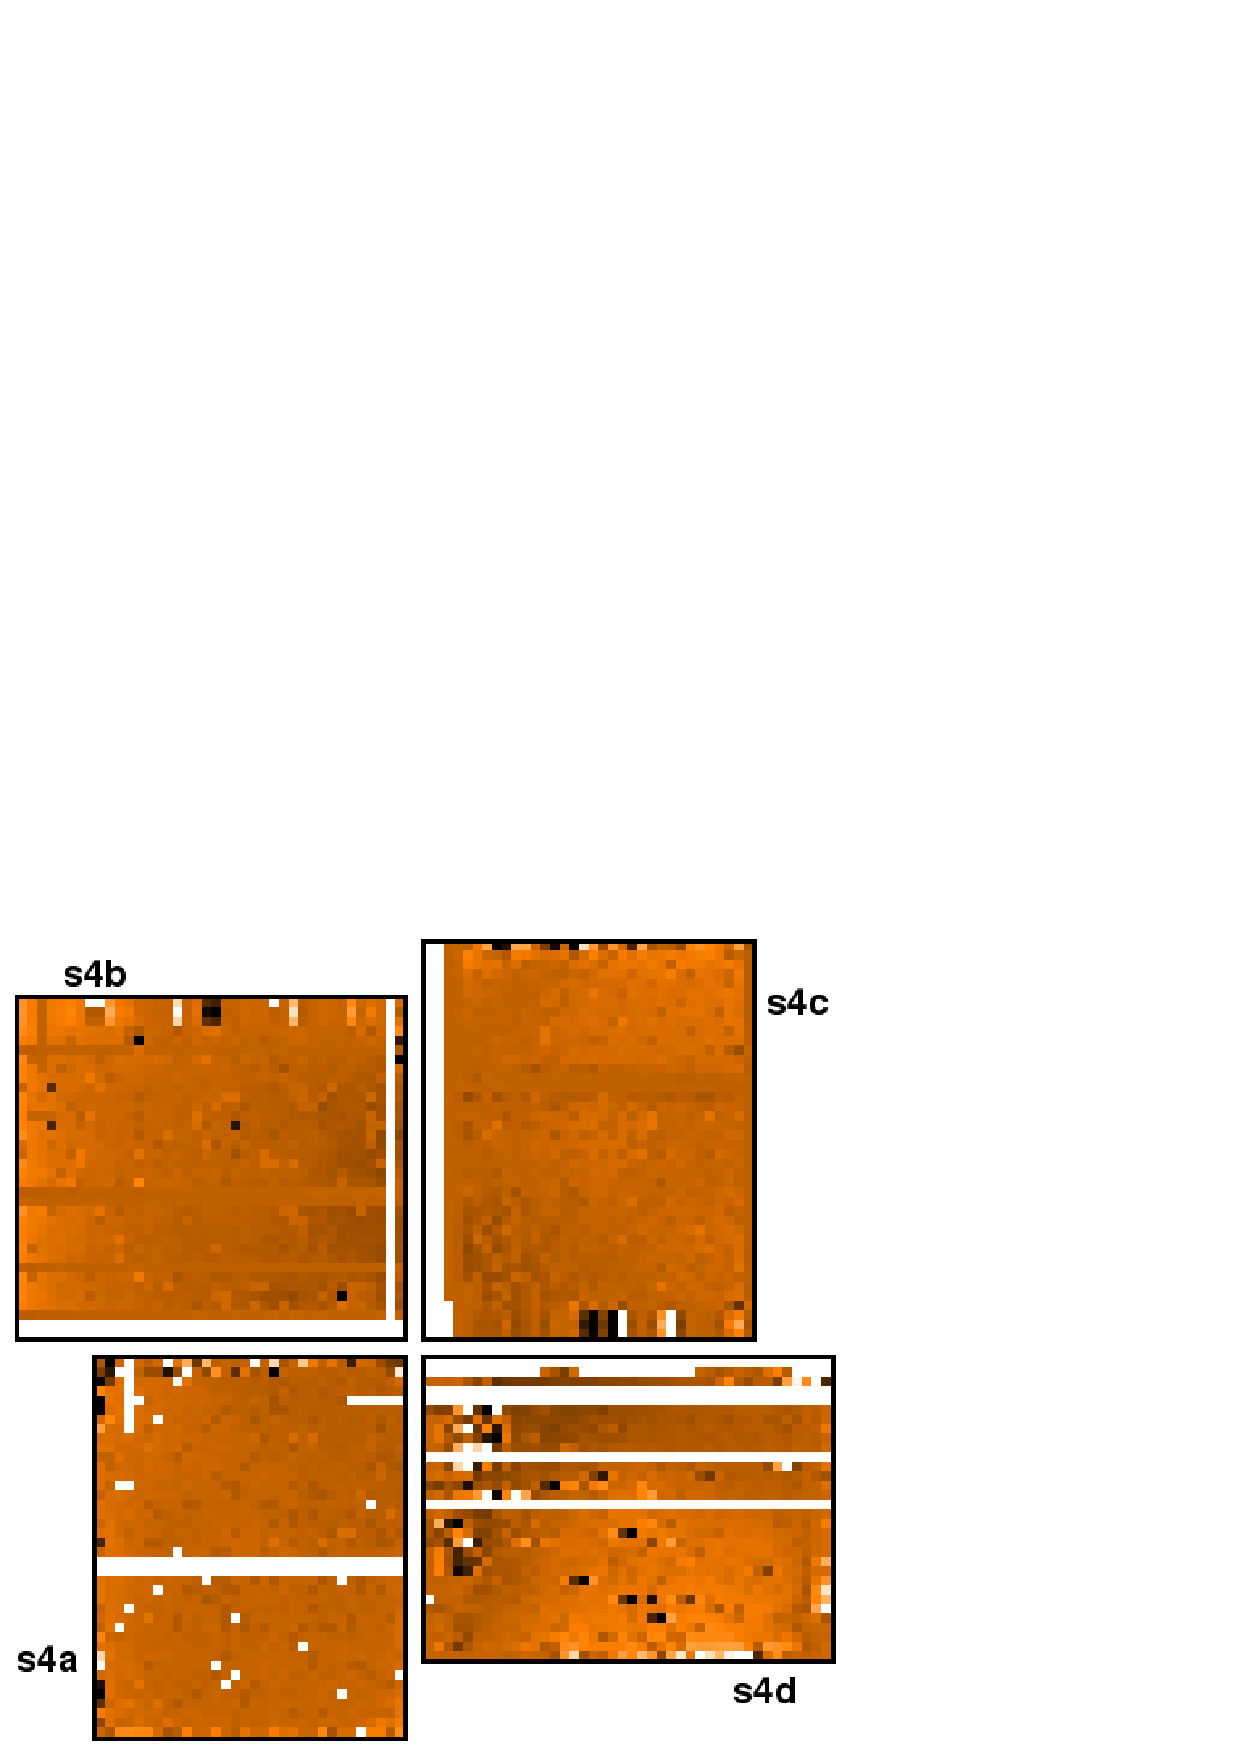
\includegraphics[width=0.4\linewidth]{sc21_450array}
\hspace{1cm}
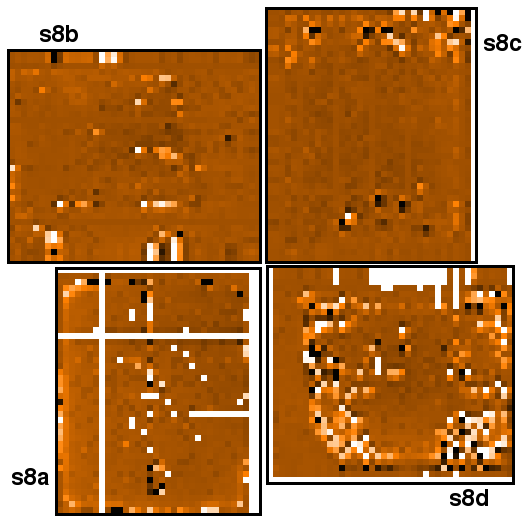
\includegraphics[width=0.4\linewidth]{sc21_850array}
\label{fig:arrays}
\caption[The physical layout of the arrays at each wavelength]{
  \small The layout of the arrays at 450$\mu$m (left) and
  850$\mu$m (right). The labels denote the name assigned to each
  sub-array. Raw data files are generated separately for each sub-array
  and must be co-added. This figure was made my running \wcsmosaic\ on
  raw files from each sub-array.
}
\end{center}
\end{figure}

\subsection{\xlabel{obs_modes}Observing modes}
\label{sec:mmodes}

Two observing modes are offered for SCUBA-2---\textsc{daisy} and
\textsc{pong}. As much of the work SCUBA-2 will be doing involves
large area mapping, both observing modes are scan patterns. Your
choice depends on the size of the area you wish to map, where you
would like your integration time concentrated and the degree of
extended emission you wish to recover

\begin{minipage}[t]{0.15\linewidth}
\textbf{PONG}
\end{minipage}
\begin{minipage}[t]{0.85\linewidth}\textsc{pong} maps are the scan
strategy for covering large areas. The default options allow for three
sizes---900\,arcsec, 1800\,arcsec and 3600\,arcsec. A single \textsc{pong} map is
a square of these dimensions and the telescope fills in the square by
bouncing off the edge of the area. To ensure an even sky background it
is recommended a minimum of three, but preferably more than five,
\textsc{pong} maps are included in a single observation with a
rotation introduced between each one. In this way a circular pattern
is built up, (see the right-hand panel of \cref{Figure}{fig:scan}{graphic below}),
with a diameter equal to your requested map size.
\vspace{0.2cm}\\
To recover large-scale extended structure you are advised to use
larger \textsc{pong} maps which scan at a higher rate. This option is
in preference to tiling multiple smaller maps. Ultimately it is the
size of the SCUBA-2 field-of-view that determines the sensitivity to
large-scale structure.
\end{minipage}
\\ \\ \\
\begin{minipage}[t]{0.15\linewidth}
\textbf{DAISY}
\end{minipage}
\begin{minipage}[t]{0.85\linewidth}
\textsc{daisy} maps are the option for point-like or compact sources
($<$3~arcmin) by maximising the exposure time on the centre of the
image. The telescope moves at a constant velocity in a `spirograph'
pattern that has the advantage of keeping the source on the array
throughout the observation. This is shown in the top panel of
\cref{Figure}{fig:scan}{the figure below}.
\end{minipage}
\vspace{1.5cm}\\
\textbf{Why these patterns?}\\*
SCUBA-2 removes atmospheric noise in the data
processing stage (Holland et al. 2013) \cite{s2main}. The power spectrum
of data taken by SCUBA-2 has a $1/f$ noise curve at lower frequencies. To
ensure astronomical signals are far away from this $1/f$ noise, fast
scanning speeds are required.

In order to disentangle source structure from other
slowly varying signals (e.g. extinction, sky noise, $1/f$ noise), the
scan pattern must pass across each region of the map from different
directions and at different times. The scan patterns themselves, along
with the associated parameters (velocity and scan-spacing), have been
designed and optimised to meet both these criteria.

\myfig{sc21_wayne_scan}{[t!]}{width=0.98\linewidth}{fig:scan}{
  Illustration of the SCUBA-2 observing patterns}{
  From left: telescope track over a single rotation of the pattern;
  telescope track after multiple rotations of the pattern; resulting
  exposure time map. The scan pattern for your observation can be
  visualised in this way with \topcat\ using the output from
  \jcmtstate.  See \cref{Section}{sec:exam}{Examining raw data} for
  more details.  Figure modified from Holland et al. (2013).
}

\clearpage

\section{\xlabel{data_files}Handling raw SCUBA-2 data}
\label{sec:raw}

This section describes a number of procedures visualising
and assessing the quality of raw data files.  These steps need not be part of
your data reduction process and do not concern the iterative map-maker.

However, there are reasons you may wish to examine your raw data in
greater depth. The most likely motivation is unusual result from the
map-maker such as higher than expected noise, artifacts in your map or
inconsistent noise across multiple tiles.  This section will help you
get to the bottom of many of these issues.

\subsection{Data acquisition explained}
A normal science observation will follow the following sequence.
\vspace{-2mm}
\begin{enumerate}\itemsep-0.2em
\item Flat-field
\item Multiple science scans
\item Flat-field
\end{enumerate}
\vspace{-2mm}
The \param{SEQ\_TYPE} parameter in the FITS header may be used to
identify the nature of each scan (see
\cref{Section}{sec:fitsheader}{Headers and file structure}).
When you access you data either at the JCMT or by downloading from the
\htmladdnormallink{Science Archive}{http://www3.cadc-ccda.hia-iha.nrc-cnrc.gc.ca/jcmt/}
\begin{latexonly}
\footnote{\texttt{http://www3.cadc-ccda.hia-iha.nrc-cnrc.gc.ca/jcmt/}}
\end{latexonly}
you will get \emph{all} of the files listed above. Later when you
reduce your data using the map-maker you will include \emph{all} of
the files (noise + flat-fields + science).
Shown below is a list of the raw files for a single sub-array (in this
case s8a) for a short calibration observation. The first file is the
short, dark noise; the second and last scans are the fast flat-field
observations which occur after the shutter opens to the sky at the
start of the observation and closes at the end (note the identical
file size); all of the scans in between are science.


\begin{myquote}
\begin{verbatim}
% ls -lh /jcmtdata/raw/scuba2/s8a/20131227/00034

-rw-r--r-- 1 jcmtarch jcmt 8.0M Dec 27 03:00 s8a20131227_00034_0001.sdf
-rw-r--r-- 1 jcmtarch jcmt  22M Dec 27 03:00 s8a20131227_00034_0002.sdf
-rw-r--r-- 1 jcmtarch jcmt  22M Dec 27 03:01 s8a20131227_00034_0003.sdf
-rw-r--r-- 1 jcmtarch jcmt  22M Dec 27 03:02 s8a20131227_00034_0004.sdf
-rw-r--r-- 1 jcmtarch jcmt  22M Dec 27 03:02 s8a20131227_00034_0005.sdf
-rw-r--r-- 1 jcmtarch jcmt 6.8M Dec 27 03:02 s8a20131227_00034_0006.sdf
-rw-r--r-- 1 jcmtarch jcmt 8.0M Dec 27 03:03 s8a20131227_00034_0007.sdf
\end{verbatim}
\end{myquote}
The SCUBA-2 data
acquisition (DA) system writes out a data file every 30 seconds; each
of which contains 22\,MB of data. The only exception is the final science
scan which will usually be smaller (6.8\,MB in the example below), typically
requiring less than 30 seconds of data to complete the observation.

\textbf{Note:} All of these files are written out eight times, once for each of
the eight sub-arrays.

The main data arrays of each file are cubes, with the first two
dimensions enumerating columns and rows, and the third time slices
(sampled at 200\,Hz).
\\*\\*
\textbf{Units}\\*
Raw SCUBA-2 data come in uncalibrated units. The first calibration
step is to scale the raw data to units proportional to picowatts (pW)
by applying the flat-field solution. This step is performed internally
 by the map-maker but can be done manually when examining the raw data---see
\cref{Section}{sec:concat}{Concatenate \& apply a flat-field}.

The second step is to scale the data by the flux conversion factor
(FCF) to give units of janskys. Unless you are running the
\textsc{Orac-dr} pipeline, this must be done manually with the
instructions given in \cref{Section}{sec:cmult}{Applying the FCF and
determining fluxes}.


\subsubsection{\xlabel{concat}Concatenate \& apply a flat-field}
\label{sec:concat}

Since SCUBA-2 data for a given sub-array are broken into multiple
30-second scans by the data acquisition (DA) system, it is useful to
concatenate the data into a single file. The \smurf\ task \concat\ can
be used for this operation. The example below combines all of the
files associated with Observation 8 for the s8a array into a single
file called \texttt{s8a20120725\_0008\_con}.

\begin{myquote}
\begin{verbatim}
% sc2concat 's8a20120725_0008*.sdf' s8a20120725_0008_con
\end{verbatim}
\end{myquote}
\task{sc2concat} will automatically filter out any dark or flat-field
observations, so that the concatenated file contains only the science
data. Be careful when concatenating a very long observation since the
output file may be too large to reasonably handle. Fifteen minute
chunks (30 files) should be sufficient.

\task{sc2concat} applies the flat-field by default (although it can be
disabled using the `noflat' option on the command-line).

The flat-field can also be applied manually using the \flatfield\ command.

\begin{myquote}
\begin{verbatim}
% flatfield 's8a20120701_0008*.sdf' '*_flat'
\end{verbatim}
\end{myquote}
Here, the output will be a flat-fielded version of each science scan
in Observation 8; the file names will be the original input
names with \_flat appended to them.

As a rule of thumb, you should apply the flat-field to your data
before examining it.


\begin{latexonly}
\begin{center}
\begin{fmpage}{0.95\linewidth}
\vspace{0.1cm}
TIP: You do not need to apply the flat-field prior to reducing your
data with the map-maker.
\end{fmpage}
\end{center}
\end{latexonly}

\begin{htmlonly}
\textbf{TIP: You do not need to apply the flat-field
prior to reducing your data with the map-maker.\\*\\*}
\end{htmlonly}


\subsection{\xlabel{header}Headers and file structure}
\label{sec:fitsheader}

There are two \Kappa\ tasks which are extremely useful for examining
your data: \fitslist\ and \ndftrace, which can be used to view the
FITS headers and dimensions of the data.
\vspace{5mm}

\begin{center}
\begin{minipage}[t]{0.12\linewidth}
\textbf{fitslist}
\end{minipage}
\begin{minipage}[t]{0.75\linewidth}This lists the FITS header information
for any file (raw or reduced). This extensive list includes dates \& times,
source name, scan type, pattern and velocity, size of the map, exposure
time, start and end elevation, opacity and the temperature of the
instrument. An example is given below:
\begin{myquote}
\begin{verbatim}
% fitslist s8a20120720_00030_000\*.sdf | grep SEQ_TYPE
\end{verbatim}
\end{myquote}
If you already know the name of the parameter you want to view you can
use the \fitsval\ command instead, e.g.\\
\begin{myquote}
\begin{verbatim}
% fitsval file.sdf TAU225ST
\end{verbatim}
\end{myquote}
\end{minipage}
\newline


\begin{minipage}[t]{0.1\linewidth} \end{minipage}
\begin{minipage}[t]{0.12\linewidth}
\textbf{ndftrace}
\end{minipage}
\begin{minipage}[t]{0.75\linewidth}
\task{ndftrace} displays the attributes of the data structure. This will tell
you the units of the data, pixel bounds, dimensions and axis assignations.
\begin{myquote}
\begin{verbatim}
% ndftrace file.sdf fullframe
\end{verbatim}
\end{myquote}
\end{minipage}
\vspace{4mm}
\end{center}

Full details of these commands can be found in the \xref{\textsc{Kappa} manual}{sun95}{}.

\begin{latexonly}
\begin{figure}[ht!]
\begin{center}
\begin{fmpage}{0.95\linewidth}
\vspace{0.2cm}
\textbf{Topcat Example}

\vspace{0.5cm}

\begin{minipage}[c]{0.6\linewidth}

\begin{myquote}
\begin{verbatim}
% topcat -f tst 20120720_30.tst
\end{verbatim}
\end{myquote}
\end{minipage}
\hspace{0.3cm}
\begin{minipage}[c]{0.32\linewidth}
Load the tst file generated by \texttt{jcmtstate2cat} into \topcat.
\end{minipage}

\vspace{0.5cm}

\begin{minipage}[c]{0.6\linewidth}
\centering
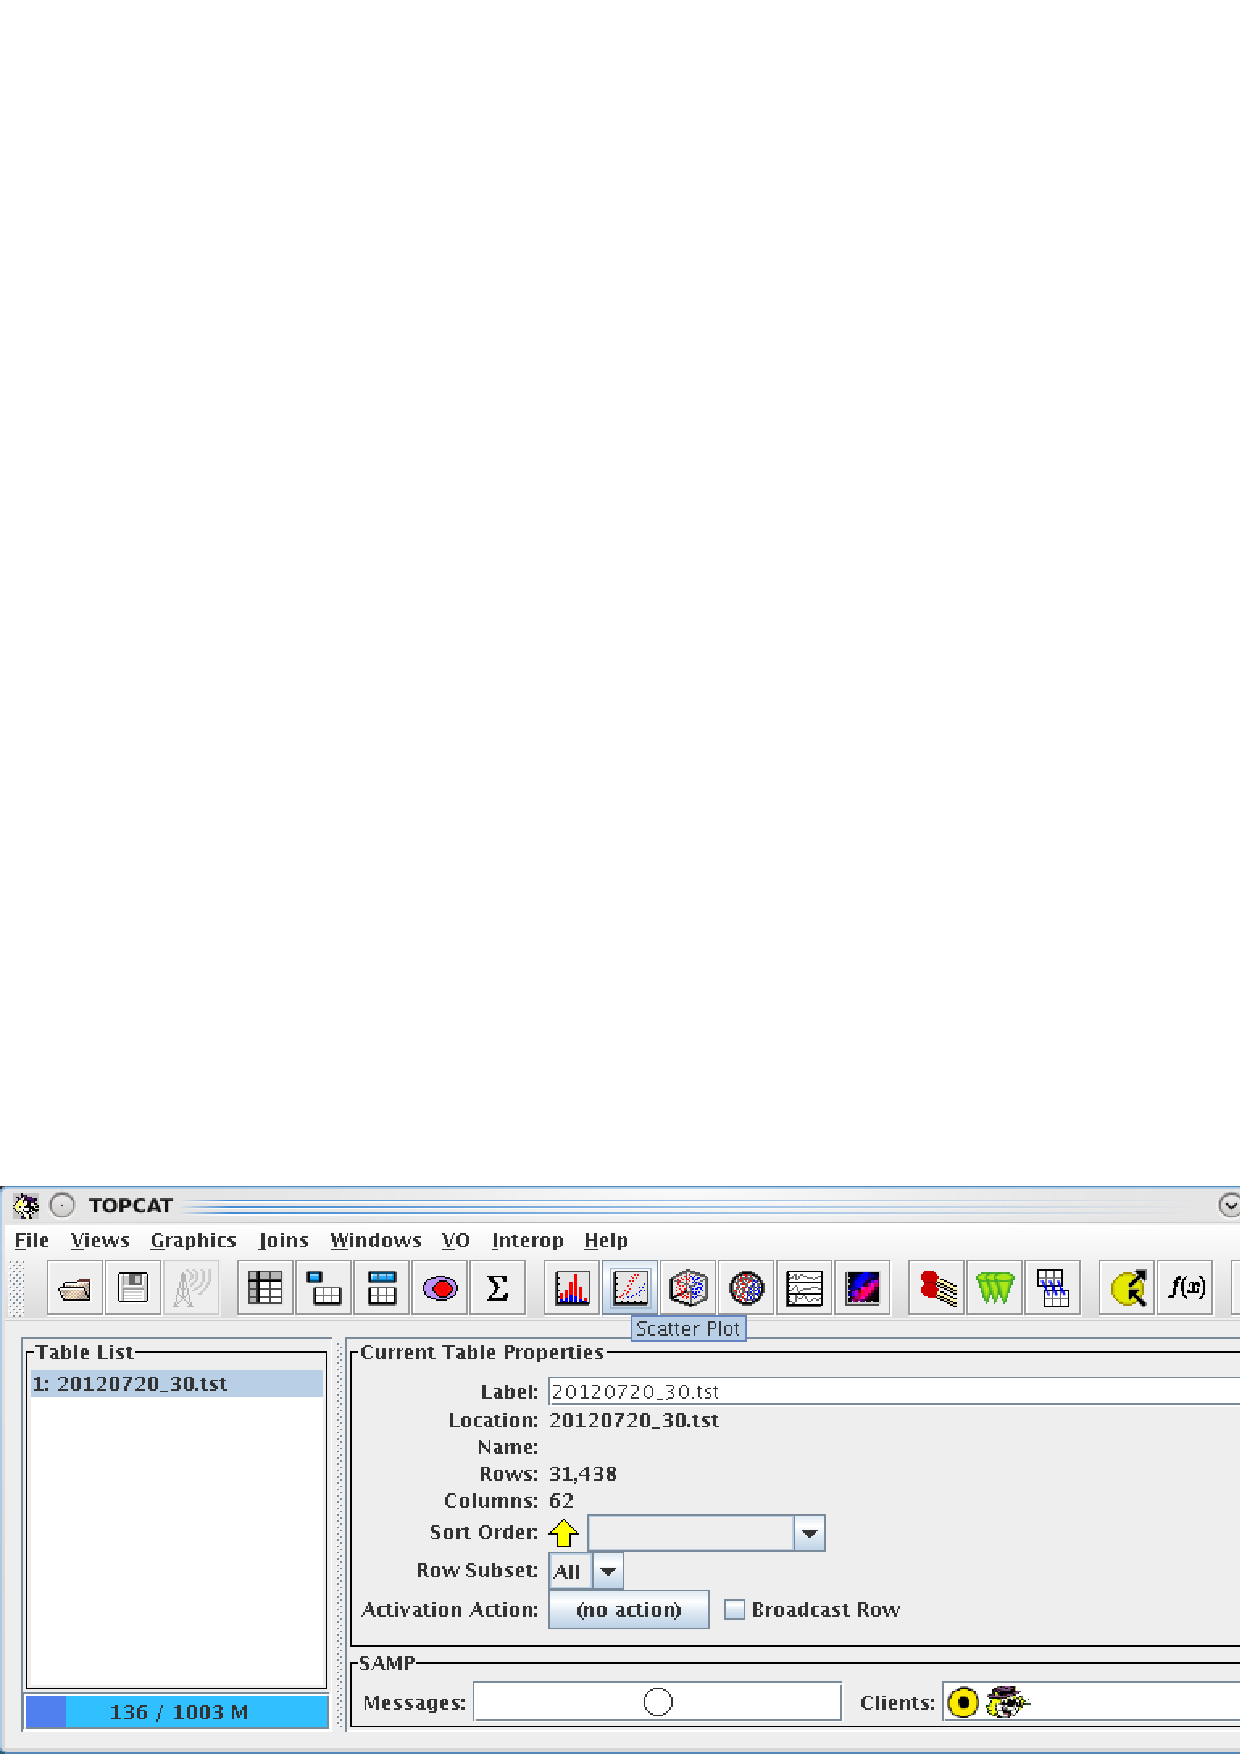
\includegraphics[width=0.95\textwidth]{sc21_topcat1}

\end{minipage}
\hspace{0.3cm}
\begin{minipage}[c]{0.32\linewidth}
In \topcat\ select the scatter plot option
from the menu bar across the top of the window.
\end{minipage}

\vspace{0.5cm}

\begin{minipage}[c]{0.6\linewidth}
\centering
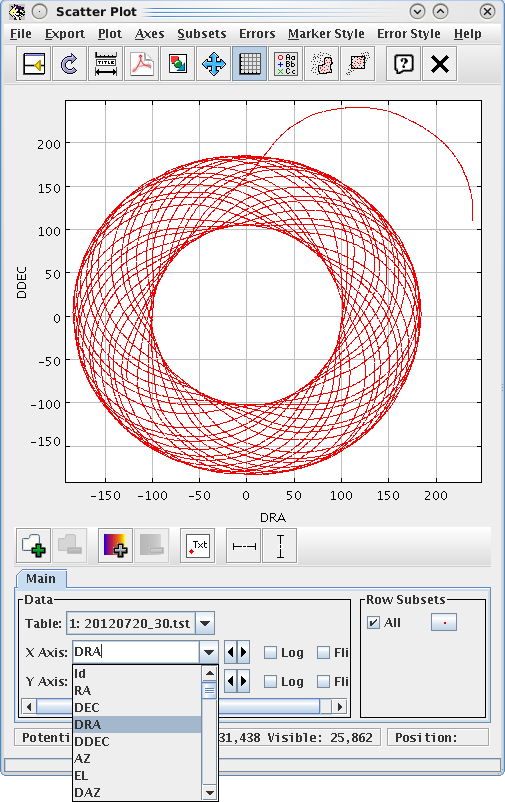
\includegraphics[width=0.75\textwidth]{sc21_topcat2}
\vspace{0.2cm}
\end{minipage}
\hspace{0.3cm}
\begin{minipage}[c]{0.32\linewidth}
With the scatter plot displayed you can adjust the $X$-axis and
$Y$-axis values to DRA and DDEC respectively to display the scan pattern.
If you are interested in seeing how any of the variables change over time,
select the the $X$ Axis to be either Id or RTS\_NUM.
\end{minipage}

\end{fmpage}
\end{center}
\caption[Displaying the scan pattern with \topcat]{
  \small \topcat\ example demonstrating how to display
  the scan pattern for an observation.
}
\label{fig:topcat}
\end{figure}
\end{latexonly}


\subsubsection{\xlabel{scan_pat}Displaying scan patterns}
\label{sec:scan}

The movement of the telescope throughout a scan (as well as other
state information) is stored in the \texttt{MORE.SMURF.JCMTSTATE}
extension of a data file. The \smurf\ task \jcmtstate\ converts this
information into a simple ASCII tab-separated table.

\begin{myquote}
\begin{verbatim}
% jcmtstate2cat s8a20120701_00008_*.sdf > state.tst
\end{verbatim}
\end{myquote}

The \texttt{-h} option to \task{jcmtstate} can be used to find more
information on the command. In particular, multiple files can be supplied
to the command using standard shell wild cards. If you have already
concatenated your data you can simply input the single concatenated
file. \textbf{It may be useful to view the scan pattern for your
observation, particularly for maps taken at high elevations, to ensure
the pattern completed successfully.}

This catalogue can be loaded into \topcat\ for plotting, making sure
to specify the TST format during loading.

\begin{myquote}
\begin{verbatim}
% topcat -f tst state.tst
\end{verbatim}
\end{myquote}

Example of scan patterns displayed with \topcat\ can be seen in
\cref{Figure}{fig:scan}{telescope tracks}. Detailed instructions on
how to display the scan pattern for your observation are given in
\cref{Figure}{fig:topcat}{box below}.
All of the time-varying header values are available for plotting. Other
values include the azimuth and elevation offsets (DAZ \& DEL), the WVM
and 225\,GHz opacity values, and the instrument temperatures (e.g.
SC2\_FPUTEMP gives the temperature of the focal plane).

% The minipages used for the dvi version give latex2html problems.
\begin{htmlonly}
 \label{fig:topcat} \htmladdimg{sc21_topcat_example.png}
 \\
 Figure: \topcat\ example demonstrating how to display the scan
 pattern for an observation.\\ \\
\end{htmlonly}

Due to extreme accelerations at ``turn-around'' points of a scan
pattern (especially for \textsc{pong}s), the telescope finds it hard
to follow the proscribed scan patterns at high elevations. To mitigate
this we try to avoid observing any sources above 70$^\circ$ elevation.
If the \fitslist\ parameters \param{ELSTART} and \param{ELEND}
indicate that your map was taken at high elevation you may consider
checking the success of the scan pattern. If you find your observation
has failed to follow the demanded scan pattern don't worry, the data is
likely to still be useful. This is especially true for \textsc{daisy}
maps where the high exposure-time central region is usually
unaffected.

\subsubsection{\xlabel{display_cube}Displaying time-series data}
\label{sec:gaiacube}

Use the \starlink\ application \textsc{Gaia} to visualise the bolometer
time-series data (or indeed \emph{any} SCUBA-2 data file). This is
initiated simply typing \texttt{gaia} into a terminal.

\begin{myquote}
\begin{verbatim}
% gaia s8a20120725_00058_con.sdf
\end{verbatim}
\end{myquote}

Loading a file in \textsc{Gaia} produces two windows (see
\cref{Figure}{fig:gaia_main}{upper graphic}). The main window shows a
map of bolometer values at a given point in time. The time slice
displayed may be changed by scrolling through the time axis. This is
done in the second window entitled \gaiathing{Display image sections of
a cube}. The \gaiathing{Index of plane} slider towards the top of this
window may be moved to display different time slices in the main
window.

\myfig{sc21_gaia1}{[b]}{width=\linewidth}{fig:gaia_main}{
  Raw data displayed in the main \gaia\ window}{
  Initial \gaia\ windows displayed upon loading a data cube.
  The main window in the left shows a map of bolometer values at a fixed
  sample in time. You may have to zoom in multiple times by clicking the
  \gaiathing{Z} icon. On the right-hand side, the
  \gaiathing{Display image sections of a cube}
  dialogue enables you to navigate the time axis.
}

A third window will appear when you click on a bolometer---the
\gaiathing{Spectral plot}. This shows an automatically scaled plot of the raw
time stream of data for that given bolometer. It will be overridden
when you click on a different bolometer.

\myfig{sc21_gaia2}{[t]}{width=0.8\linewidth}{fig:gaia_spec}{
  \gaia\ spectral plot window}{
  The \gaiathing{Spectral plot} window displays the time-varying signal. This window
  appears automatically when a bolometer is clicked in the main window.
  The vertical red line indicates the time slice that is currently selected
  in the \gaiathing{Display image sections of a cube} dialogue---this can be
  dragged across the spectrum to scroll through the time-slices.
}

A second way to scroll through the time axis is to click and drag the
vertical red bar on the \gaiathing{Spectral plot} window. As you do
so, the array shown in the main window will automatically update.

To highlight small variations between bolometers it is likely you will
need to change the auto cut and (depending on your preference) the
colour scheme---both are controlled by buttons on the sidebar.

See the \xref{\textsc{Gaia} manual}{sun214}{} for full
details.\latex{\footnote{\texttt{http://docs.jach.hawaii.edu/star/sun214.htx/sun214.html}}}

\clearpage
\subsection{\xlabel{regrid_map}Regridding data into a map}
\label{sec:regrid}

Any raw time-series data can be quickly regridded into sky frame
coordinates using the \smurf\ \makemap\ task in rebin mode. This
involves no processing of the data. The following command produces a
map from the raw concatenated data; unlike the iterative mode of
\task{makemap} described in the next chapter, no configuration file is
required.
\begin{myquote}
\begin{verbatim}
% makemap s8a20120725_00058_con.sdf crl2688_sky method=rebin
\end{verbatim}
\end{myquote}
The output map here is called \texttt{crl2688\_sky.sdf} and is shown
in \cref{Figure}{fig:regrid}{the figure below}.
The pixel scale is left at the default values of 2\,arcsec on a side at
450$\mu$m and 4\,arcsec at 850$\mu$m (although this can be changed
using the \texttt{pixsize=}$x$ option on the command-line, where $x$ is in
arcsec).

\myfig{sc21_crl2688_regrid}{[b!]}{width=0.65\linewidth}{fig:regrid}{
  The regridded map of CRL2688 displayed with \gaia.}{
  The regridded map of CRL2688 with the s8a sub-array displayed with \gaia.
}

\begin{latexonly}
\begin{center}
\begin{fmpage}{0.95\linewidth}
\vspace{0.1cm}
TIP: If you do not include method=rebin, the map-maker will will default to method=iterate.
\end{fmpage}
\end{center}
\end{latexonly}

\begin{htmlonly}
\textbf{TIP: If you do not include method=rebin, the map-maker will
default to method=iterate.\\*\\*}
\end{htmlonly}


\subsection{\xlabel{clean}Notes on cleaning your data}
\label{sec:clean}

Cleaning raw data is an essential first step towards making a quality
final map. The map-maker performs all of these cleaning steps during
the pre-processing stage. The commands for manually cleaning your data
are given in \cref{Appendix}{app:clean}{Cleaning the Raw Data}.

% Split to avoid paragraph break mid-sentence.
\begin{htmlonly}
You can also check out the \xref{SMURF SRO Cookbook}{sc19}{} which
goes into great depth on the data cleaning options.
\end{htmlonly}
\begin{latexonly}
You can also check out the SMURF SRO
Cookbook{\footnote{\texttt{http://www.starlink.ac.uk/docs/sc19.htx/sc19.html}}}
which goes into great depth on the data cleaning options.
\end{latexonly}


\subsection{\xlabel{calcnoise}Checking the array performance}
\label{sec:calcnoise}

The on-sky performance of the array can be assessed using the \smurf\
command \calcnoise. Rather than give an absolute measure, \task{calcnoise}
should be used as an indicator of array performance and stability.
\task{calcnoise} cleans the data then calculates the
white noise on the array (between 2 and 10\,Hz by default). If the
dark noise scans are given as input, this will track the array
sensitivity independent of sky conditions. If you provide the whole
observation (as in the example below) then the dark files will be
ignored and the on-sky performance of the array is calculated.

\begin{myquote}
\begin{verbatim}
% calcnoise s8a20110720_00030*.sdf s8a_noise method=! power=!
\end{verbatim}
\end{myquote}
It will prompt for a configuration file to describe the cleaning
steps---the default is the supplied \texttt{dimmconfig\_calcnoise.lis}.
Two noise measurements are reported in the terminal: the
`Effective noise' and the `Effective NEP'.

An output file is created for each sub-array with the NEP map stored
in the \texttt{.MORE.SMURF.NEP} extension.

If you have a bright source in the field this will
contaminate the signal. In this case you should examine the
\texttt{NOI} model from the map-maker instead---see
\cref{Section}{sec:models}{The Individual Models} for a description
and \cref{Section}{sec:export}{Exporting individual models} for
details on how to examine it.

\clearpage
\section{\xlabel{dimm}The Dynamic Iterative Map-Maker Explained}
\label{sec:dimm}

The Dynamic Iterative Map-Maker (DIMM), hereafter just referred to as
the map-maker is the tool you will use to produce SCUBA-2 maps. It
performs all pre-processing steps to clean the data, followed by
iteratively solving for multiple signal components and regridding to
produce a final science map.

This section describes how the map-maker produces a science images
from raw SCUBA-2 data. It is essential reading to gain an
understanding of what has happened to produce your reduced image,
especially if you wish to modify the default map-maker parameters.
\color{red} If you prefer to jump straight in to the data reduction go
to \cref{Section}{sec:maps}{Reducing your data}.\color{black}


\subsection{\xlabel{dimm_theory}How it works}

The map-maker works by individually modelling the various
contributions that make up the signal recorded by each bolometer. It
models and then subtracts all the sources of signal in order of
decreasing magnitude, ultimately leaving just the astronomical signal
plus noise. A list of the modelled components can be seen in
\cref{Table}{tab:mods}{tabulated} and a description found in
\cref{Section}{sec:models}{The Individual Models}.

\textbf{The map-maker requires a configuration file to accompany each
reduction.} This file instructs the map-maker on the pre-processing
steps, which components to iteratively model, the parameters to use
when doing so, and finally the stopping (or convergence) criteria.
There is a single `master' configuration
file called \texttt{dimmconfig.lis}. A copy of this file is available in
\cref{Appendix}{app:dimm}{an appendix}.

Often, the default configuration file will not give optimal results
for your particular observation. For this reason, specialised
configuration files have been developed which are tailored to
different science goals, be they detecting faint galaxies or mapping
large molecular clouds. A
description of these specialised configuration files can be found
\cref{in Section}{sec:config}{here}.

\subsection{The Reduction Step-by-Step}

\textbf{This description applies to the default configuration file -
\texttt{dimmconfig.lis}.}\\*\\* \cref{Figure}{fig:dimm}{The graphic
below} shows the flow chart of the map-making process
for \texttt{dimmconfig.lis}. It is divided into two sections: the
pre-processing stage where the data are cleaned, then the iterative
stage where the different models are subtracted and the convergence checked.
\cref{Table}{tab:dimmdef}{A table of active variables} gives all the
configuration parameters in \texttt{dimmconfig.lis} again, divided
into the two main stages.

\begin{center}
\begin{minipage}[t]{0.95\linewidth}
\textbf{1. Initial cleaning and downsampling}\\
The first task the map-maker perform is to down-sample the data. The
raw time-series data is re-sampled at a rate that matches the
requested pixel size, the equivalent to applying a low-pass filter.
Down-sampling saves time and memory usage when running the map-maker.
The raw data is then concatenated and has the flat-field (from the
bracketing fast flat scans) applied to calibrate the bolometers. A
number of cleaning steps are then run: a polynomial baseline is
subtracted from each bolometer; spikes and dc steps are removed; any
resulting gaps in the time-series are filled in.
\\*\\*
\textbf{2. Iterative steps}\\
Next comes the iterative stage of the process. First to be modelled
and removed are \texttt{COM} and \texttt{GAI} which work together to
calculate the average signal template of all the bolometers, and then
fit/remove the templates from each bolometer. The next model
(\texttt{EXT}) applies a multiplicative extinction correction to the
data. Following this, a Fourier transform is applied to the data and
the \texttt{FLT} model is removed in the frequency domain.
\texttt{FLT} applies a high-pass filter to the data, above frequencies
that correspond to angular scales of 600\,arcsec and 300\,arcsec at
450$\mu$m and 850$\mu$m, respectively.
\\\\
The first step in creating the  \texttt{AST} model involves
regridding the data to produce an estimation of the final science map.
Since many samples typically contribute to the estimate of the signal
in a given pixel, the noise is greatly reduced compared with the
time-series data. This map is then projected back into the time series
and the \texttt{AST} model removed. The \texttt{NOI} model then
measures the noise in the residual signals for each bolometer to
establish weights for the data as they are placed into the map in
subsequent iterations.
\\*\\*
\textbf{3. Checking convergence}\\
At this stage convergence is checked against the parameters detailed
in the configuration file. Convergence is achieved either when the
requested number of iterations has been completed or when the
noise-based convergence criteria specified in the configuration file
is reached. If more iterations are required or (in the latter case)
the residual noise has not converged then \texttt{GAI}, \texttt{EXT},
\texttt{FLT} and \texttt{COM} models are all undone and the
time-series is reconstructed. The sequence is then rerun only this
time without \texttt{AST} complicating the model fitting.
\end{minipage}
\end{center}

\myfig{sc21_flow_dimm_blue}{}{width=0.78\linewidth}{fig:dimm}{
  Flowchart of the map-maker}{
  A flow chart illustrating the dynamic iterative map-maker. Note that
  for each iteration the \texttt{AST} model is subtracted from the
  time-series leaving only those contributions to be fitted and
  removed.
}

For full details of the map-maker see \textbf{Chapin et al. (2013)} \cite{mapmaker}.
\begin{latexonly}
\setlength{\extrarowheight}{3pt}
\begin{table}
\centering
\begin{tabular}{c|l}
\hline
\textbf{Model} &\hspace{0.2cm} \textbf{Description} \\
\hline
\texttt{COM}&\hspace{0.2cm} Common-mode signal\\
\texttt{GAI}&\hspace{0.2cm} Common-mode scaled to each bolometer---the gain\\
\texttt{EXT}&\hspace{0.2cm} Extinction correction\\
\texttt{FLT}&\hspace{0.2cm} Fourier transform filter\\
\texttt{AST}&\hspace{0.2cm} Map estimate of astronomical signal\\
\texttt{NOI}&\hspace{0.2cm} Noise estimation\\
\hline
\end{tabular}
\label{tab:mods}
\caption{\small Table adopted from Chapin et al. (2013). A detailed
explanation of each model is given in \cref{Section}{sec:models}{The individual models}.}
\end{table}
\end{latexonly}

\raggedbottom
\subsection{\xlabel{models}The individual models}
\label{sec:models}

The particular sequence of the models evaluated (and removed) by the
map-maker during the iterative stage is indicated by the
\texttt{modelorder} parameter in the configuration file. These models
are modular however so their order may be changed. The default model
order in \texttt{dimmconfig.lis} is given below.

\begin{myquote}
\begin{verbatim}
modelorder = (com,gai,ext,flt,ast,noi)
\end{verbatim}
\end{myquote}

The only recipe not following this model order is the one tailored for
blank field maps which does not include a \texttt{FLT} model in the
iterative stage (see \cref{Section}{sec:config}{Specialised
configuration files}).

Below is an introduction to each model. More complete descriptions of the
models and all the associated caveats can be found in Chapin et al.
(2013) \cite{mapmaker}.
\begin{htmlonly}
\setlength{\extrarowheight}{3pt}
\begin{table}[t!]
\centering
\begin{tabular}{c|l}
\hline
\textbf{Model} &\hspace{0.2cm} \textbf{Description} \\
\hline
\texttt{COM}&\hspace{0.2cm} Common-mode signal\\
\texttt{GAI}&\hspace{0.2cm} Common-mode scaled to each bolometer---the gain\\
\texttt{EXT}&\hspace{0.2cm} Extinction correction\\
\texttt{FLT}&\hspace{0.2cm} Fourier transform filter\\
\texttt{AST}&\hspace{0.2cm} Map estimate of astronomical signal\\
\texttt{NOI}&\hspace{0.2cm} Noise estimation\\
\hline
\end{tabular}
\label{tab:mods}
\caption{\small Table adopted from Chapin et al. (2013). A detailed
explanation of each model is given in \cref{Section}{sec:models}{The individual models}.}
\end{table}
\end{htmlonly}
\\ \\
\hrule
\begin{minipage}[t]{0.12\linewidth}
\centering\textbf{MODEL}
\end{minipage}
\begin{minipage}[t]{0.88\linewidth}
\centering\textbf{DESCRIPTION}
\end{minipage}
\hrule
%\vspace{0.1cm}
\begin{minipage}[t]{0.12\linewidth}
\centering\texttt{COM}
\end{minipage}
\begin{minipage}[t]{0.88\linewidth}The \texttt{COM} model removes the
common-mode signal (the signal that is common to all bolometers), the
dominant contributor to this signal being the sky noise. It determines
this by simply averaging over all bolometers for each time slice.
Bolometers are flagged as bad, (and thus omitted from the final map), if
they do not resemble the \texttt{COM} model seen by the majority of the
other bolometers.
\newline Extended emission on a scale larger than the array footprint
on the sky will contribute a signal indistinguishable from a
common-mode signal. This puts an upper limit on the spatial scale of
astronomical emission that can be recovered. \\
\end{minipage}
\hrule
\vspace{0.1cm}
\begin{minipage}[t]{0.12\linewidth}
\centering\texttt{GAI}
\end{minipage}
\begin{minipage}[t]{0.88\linewidth}The \texttt{GAI} model works with
\texttt{COM} in removing the common-mode signal. \texttt{GAI} is used to
scale the \texttt{COM} model that has been subtracted and is described by
a gain and an offset to scale all the bolometers to the same level. This
will allow the bolometers to share a common calibration further down the
line. \\
\end{minipage}
\hrule
\vspace{0.1cm}
\begin{minipage}[t]{0.12\linewidth}
\centering\texttt{EXT}
\end{minipage}
\begin{minipage}[t]{0.88\linewidth}\texttt{EXT} applies the extinction
correction. This is a time-varying scaling factor that is derived from
the JCMT water-vapour radiometer. As it deals with 30-second chunks of
data this accounts for varying conditions over a long observation. For
more details see \cref{Appendix}{app:cal}{SCUBA-2 data calibration}. \\
\end{minipage}
\hrule
\vspace{0.1cm}
\begin{minipage}[t]{0.12\linewidth}
\centering\texttt{FLT}
\end{minipage}
\begin{minipage}[t]{0.88\linewidth}The \texttt{FLT} model acts on the FFT
of the bolometer data. High-pass (only allows \textit{higher} frequencies to
pass) and low-pass (only allows \textit{lower} frequencies to pass) filters
can be specified. These cut-off frequencies can either be be specified by
you directly or as an angular spatial scale (which is subsequently
converted into a frequency dependent on the speed at which the
telescope is moving). The most important role of this model is to
apply a high-pass filter in order to remove the $1/f$ noise. Note that
extended emission varies slowly over the array; it therefore appears
at low frequencies and complicates the choice of a high-pass filter. A
further discussion of this matter is given in
\cref{Section}{sec:bright_ex}{Extended galactic sources}\\
\end{minipage}
\hrule
\vspace{0.1cm}
\begin{minipage}[t]{0.12\linewidth}
\centering\texttt{AST}
\end{minipage}
\begin{minipage}[t]{0.88\linewidth}This step involves both the creation of the
\texttt{AST} model and the final science map. Hence, the position of
\texttt{AST} in the model order indicates at what stage the astronomical
image should be estimated. When the \texttt{AST} model is called, the first
step is regridding the raw time-series data, (using nearest-neighbour sampling),
to produce an estimate of the final map. Following this, the map is
projected back into the time domain and removed (as the \texttt{AST}
model).\\
\end{minipage}
\hrule
\vspace{0.1cm}
\begin{minipage}[t]{0.12\linewidth}
\centering\texttt{NOI}
\end{minipage}
\begin{minipage}[t]{0.88\linewidth}\texttt{NOI} should come last in the model
order and calculates the RMS noise in each bolometer.  \texttt{NOI} is
determined by running \calcnoise\ (see \cref{Section}{sec:calcnoise}{Checking the
array performance}) on the residual signal (the \texttt{RES}
model, see \cref{Section}{sec:export}{Exporting individual models}).  Unlike
the other models, \texttt{NOI} is
not a subtraction or a correction but if specified, is used (from the
second iteration onwards) to weight the bolometers in the map
estimate.\\
\end{minipage}
\hrule

\subsection{\xlabel{convergence}Stopping criteria}
\label{sec:converge}

The map-maker will stop processing either when the requested number of
iterations has been completed \textbf{OR} when the convergence
criteria specified in the configuration file is reached.
\\*\\*
\textbf{Option 1: Fixed number of iterations}\\*
Specifying the number of iterations in the configuration file is done via
the \texttt{numiter} parameter. In \texttt{dimmconfig.lis}, this is given
by:
\vspace{-0.1cm}
\begin{myquote}
\begin{verbatim}
numiter = -5
\end{verbatim}
\end{myquote}
\vspace{-0.1cm}
A positive value for \texttt{numiter} means that the requested number
of iterations will be executed. A negative value, as in the example
above, indicates that no more than this number of iterations should be
performed, \emph{but} that it may stop at fewer if convergence
(according to the noise criteria below) has been achieved.
\\*\\*
\textbf{Options 2: Convergence parameter}\\*
The convergence criteria is set by the \textbf{maptol} parameter.

When running the map-maker, \texttt{maptol} gives the average
normalised change in the value of map pixels
between subsequent iterations. Convergence is reached when the change
is less than the parameter \texttt{maptol}. It has units of the noise
in the map, thus \texttt{maptol}$=$0.05 means a change of
$<$0.05\,$\sigma$. This option has the advantage of directly assessing
the noise in the resulting map rather than the time-series.

Typically the normalized change in pixel values between iterations
drops rapidly to begin with and then flattens out, decreasing
increasingly slowly. As a result, in some circumstances, the map-maker
will fail to stop iterating due to low frequency ripples coming and
going between iterations.
\vspace{3mm}\\
\texttt{maptol}~=~0.05 is the default. Be aware that
setting \texttt{maptol} to lower than 0.05 will dramatically increase
the length of time to produce the final map and possibly never achieve
convergence. [RECOMMENDED]
\vspace{2mm}


The best way of checking the progress of convergence while running the
map-maker is to use the \param{itermap} option and setting
\param{itermap~=~1} (see \cref{Section}{sec:tweak}{Tweaking the
Configuration File}).

\begin{figure}
\begin{center}
\begin{latexonly}
  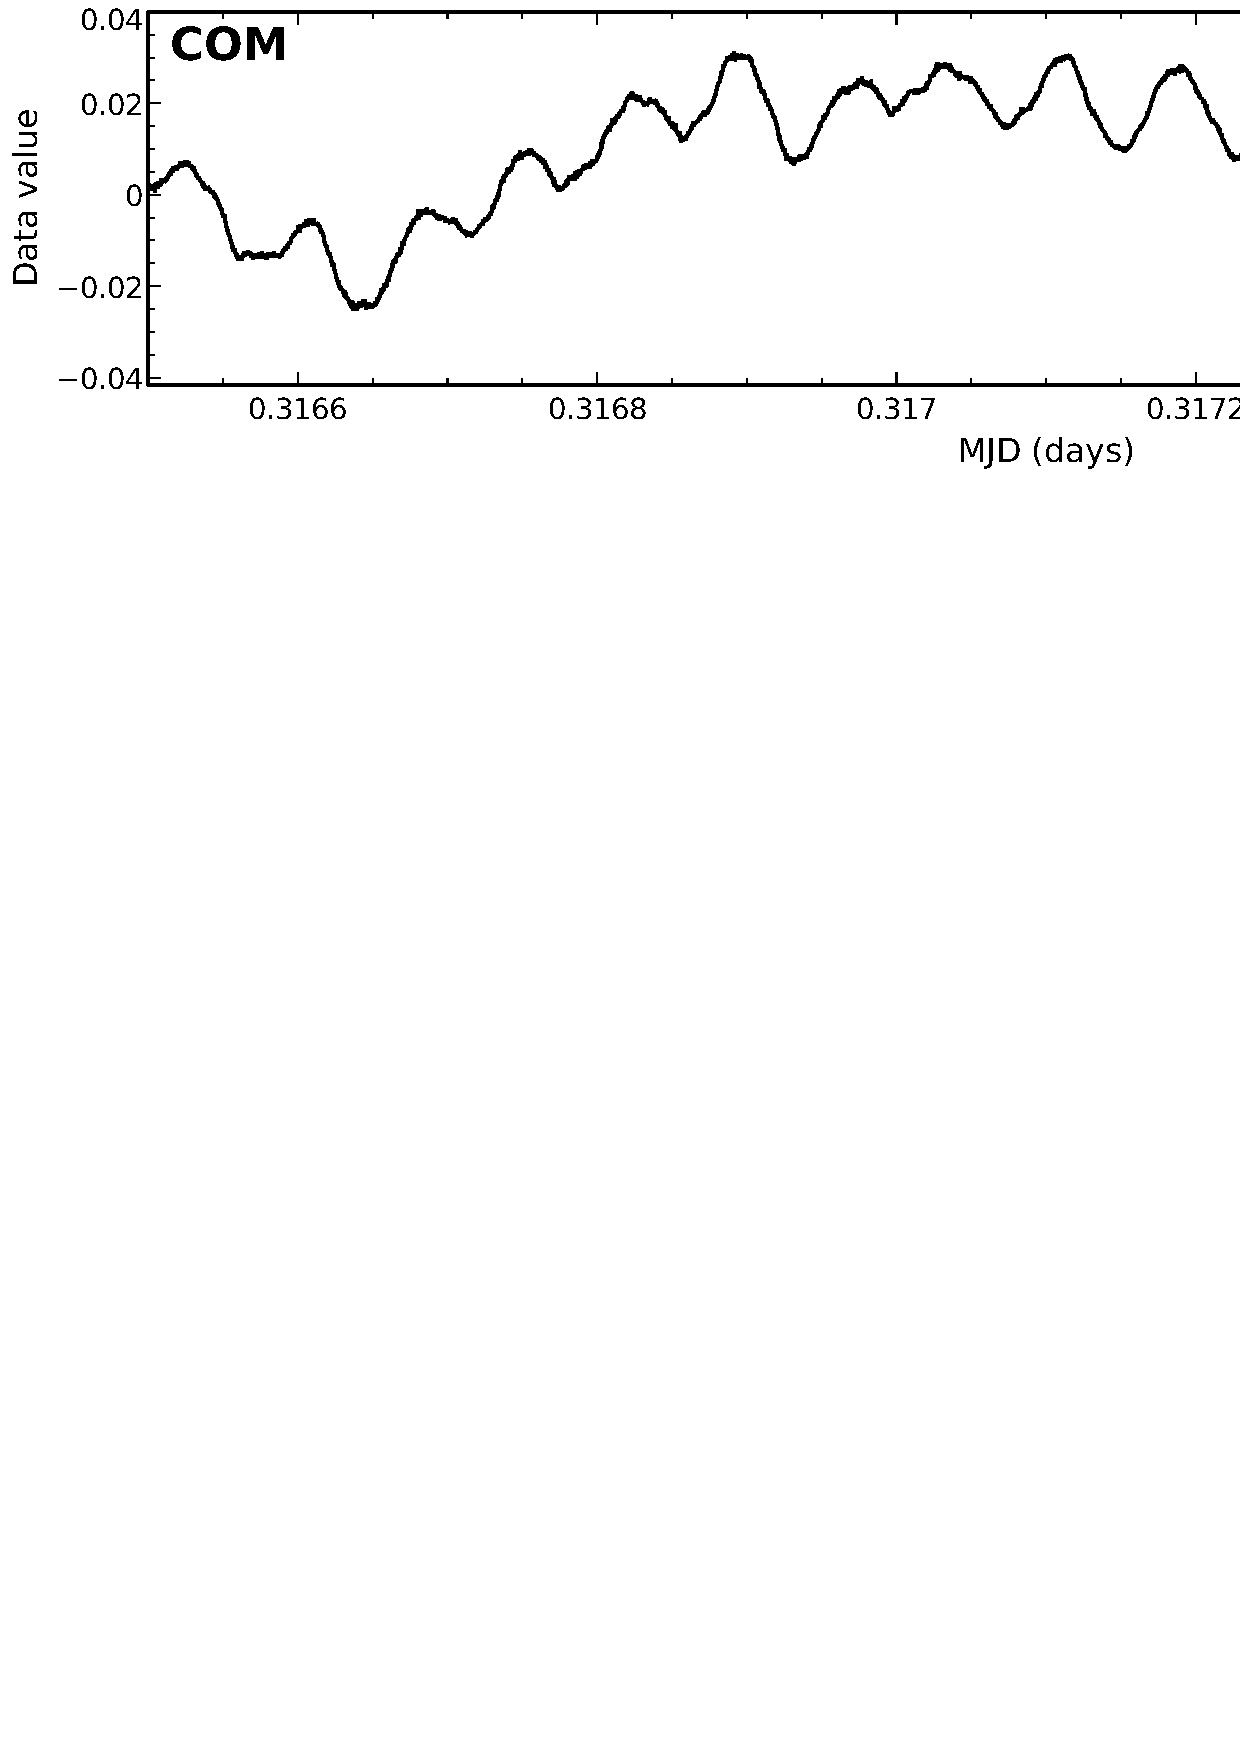
\includegraphics[width=\linewidth]{sc21_com} \\
  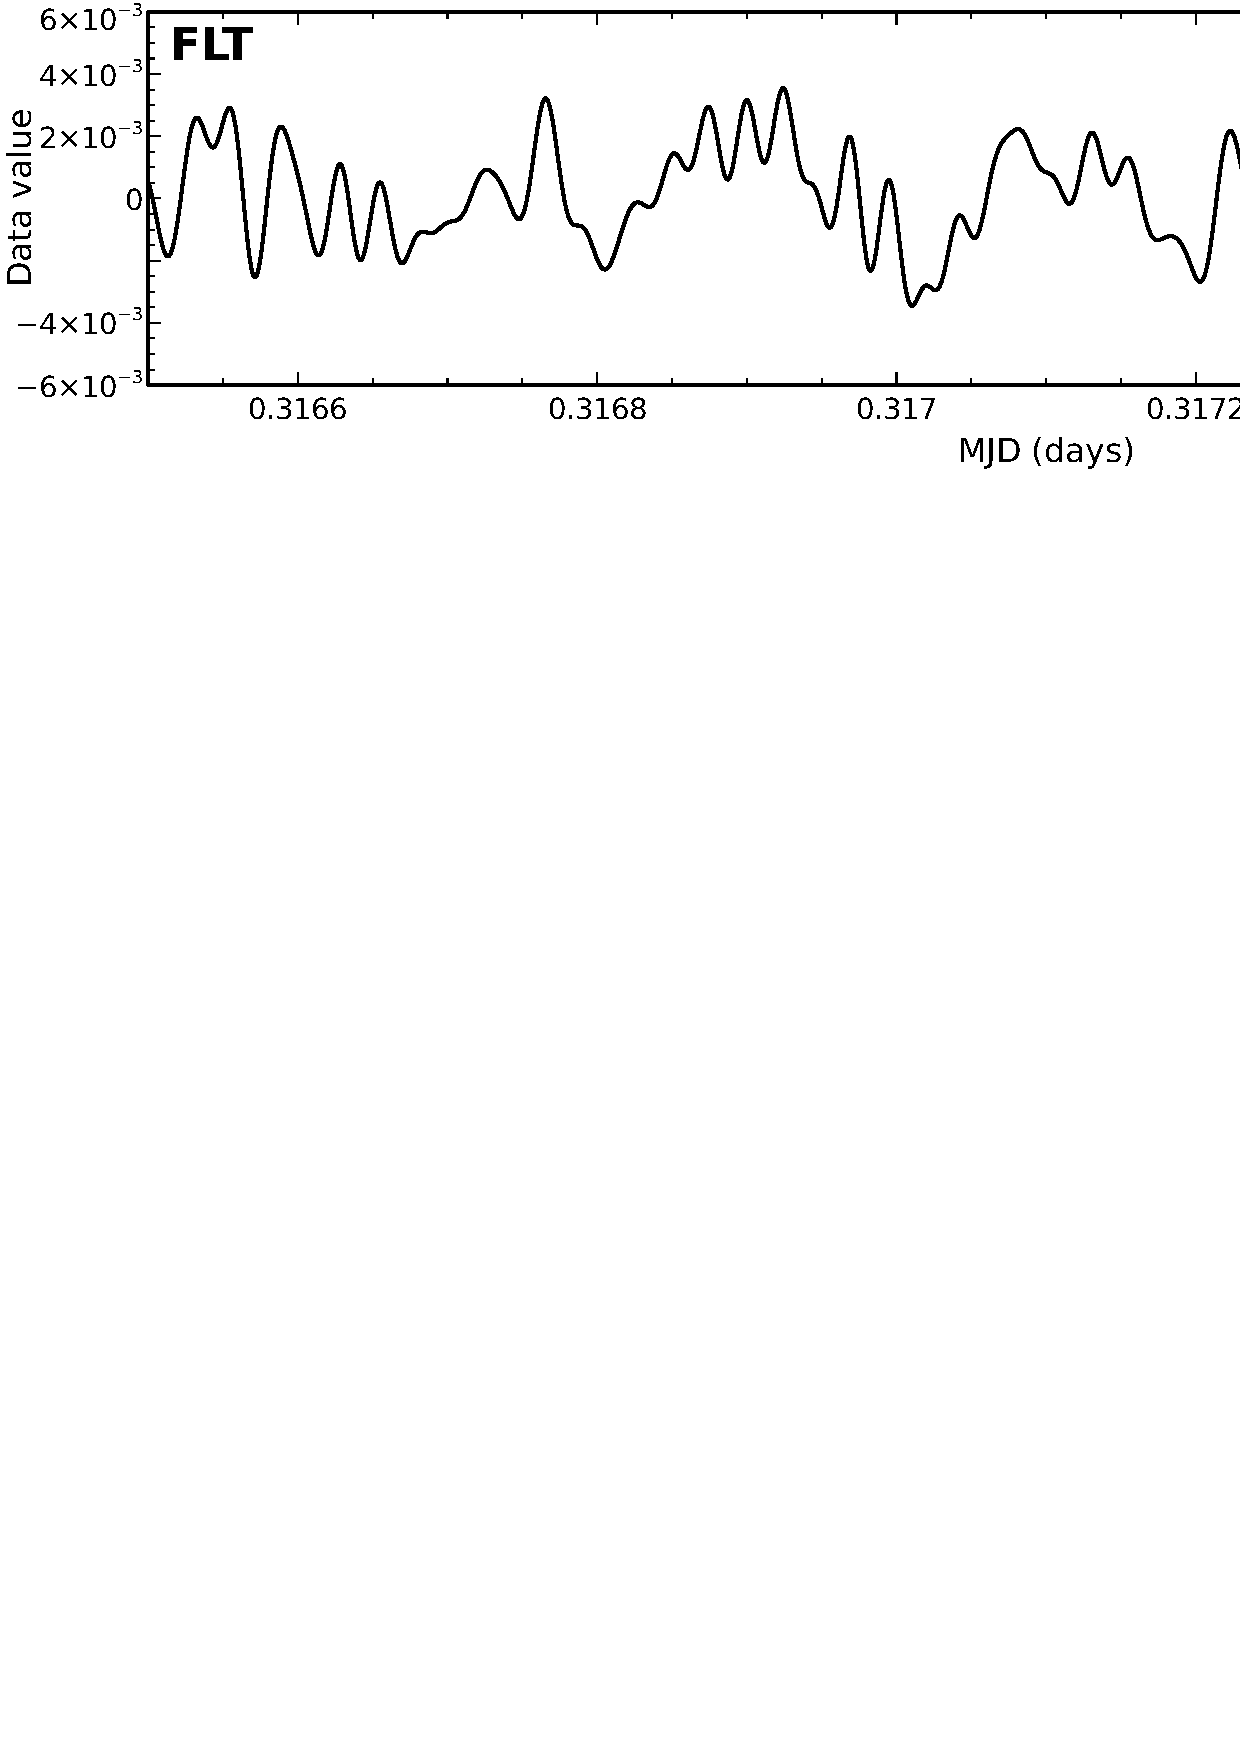
\includegraphics[width=\linewidth]{sc21_flt} \\
  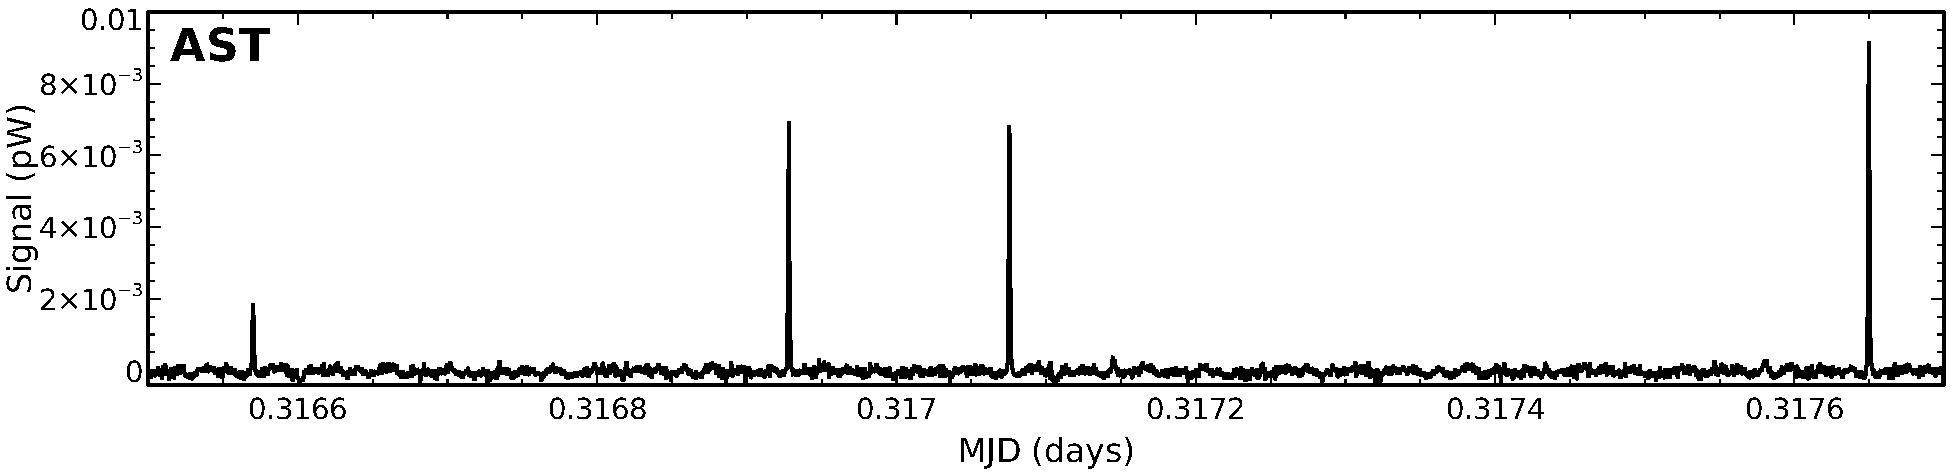
\includegraphics[width=\linewidth]{sc21_ast} \\
  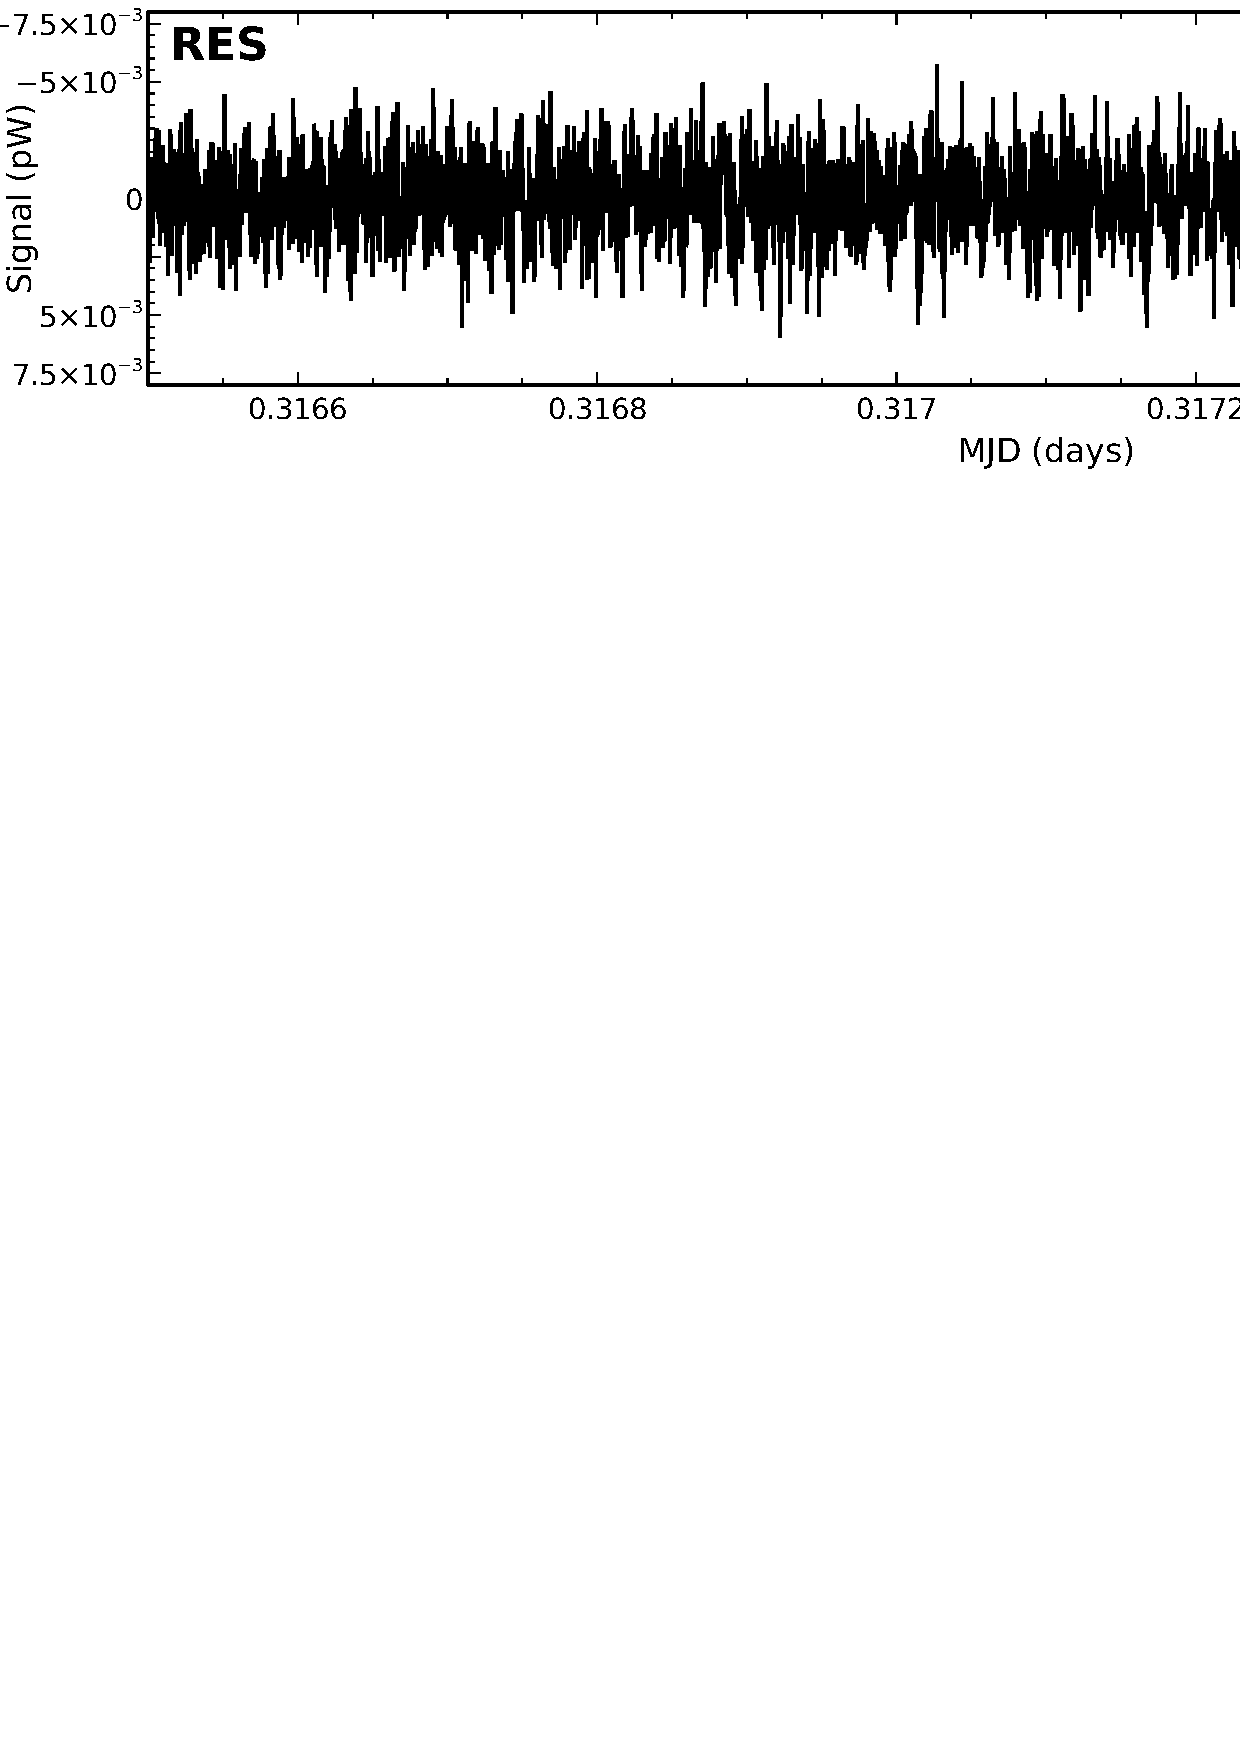
\includegraphics[width=\linewidth]{sc21_res} \\
\end{latexonly}
\begin{htmlonly}
  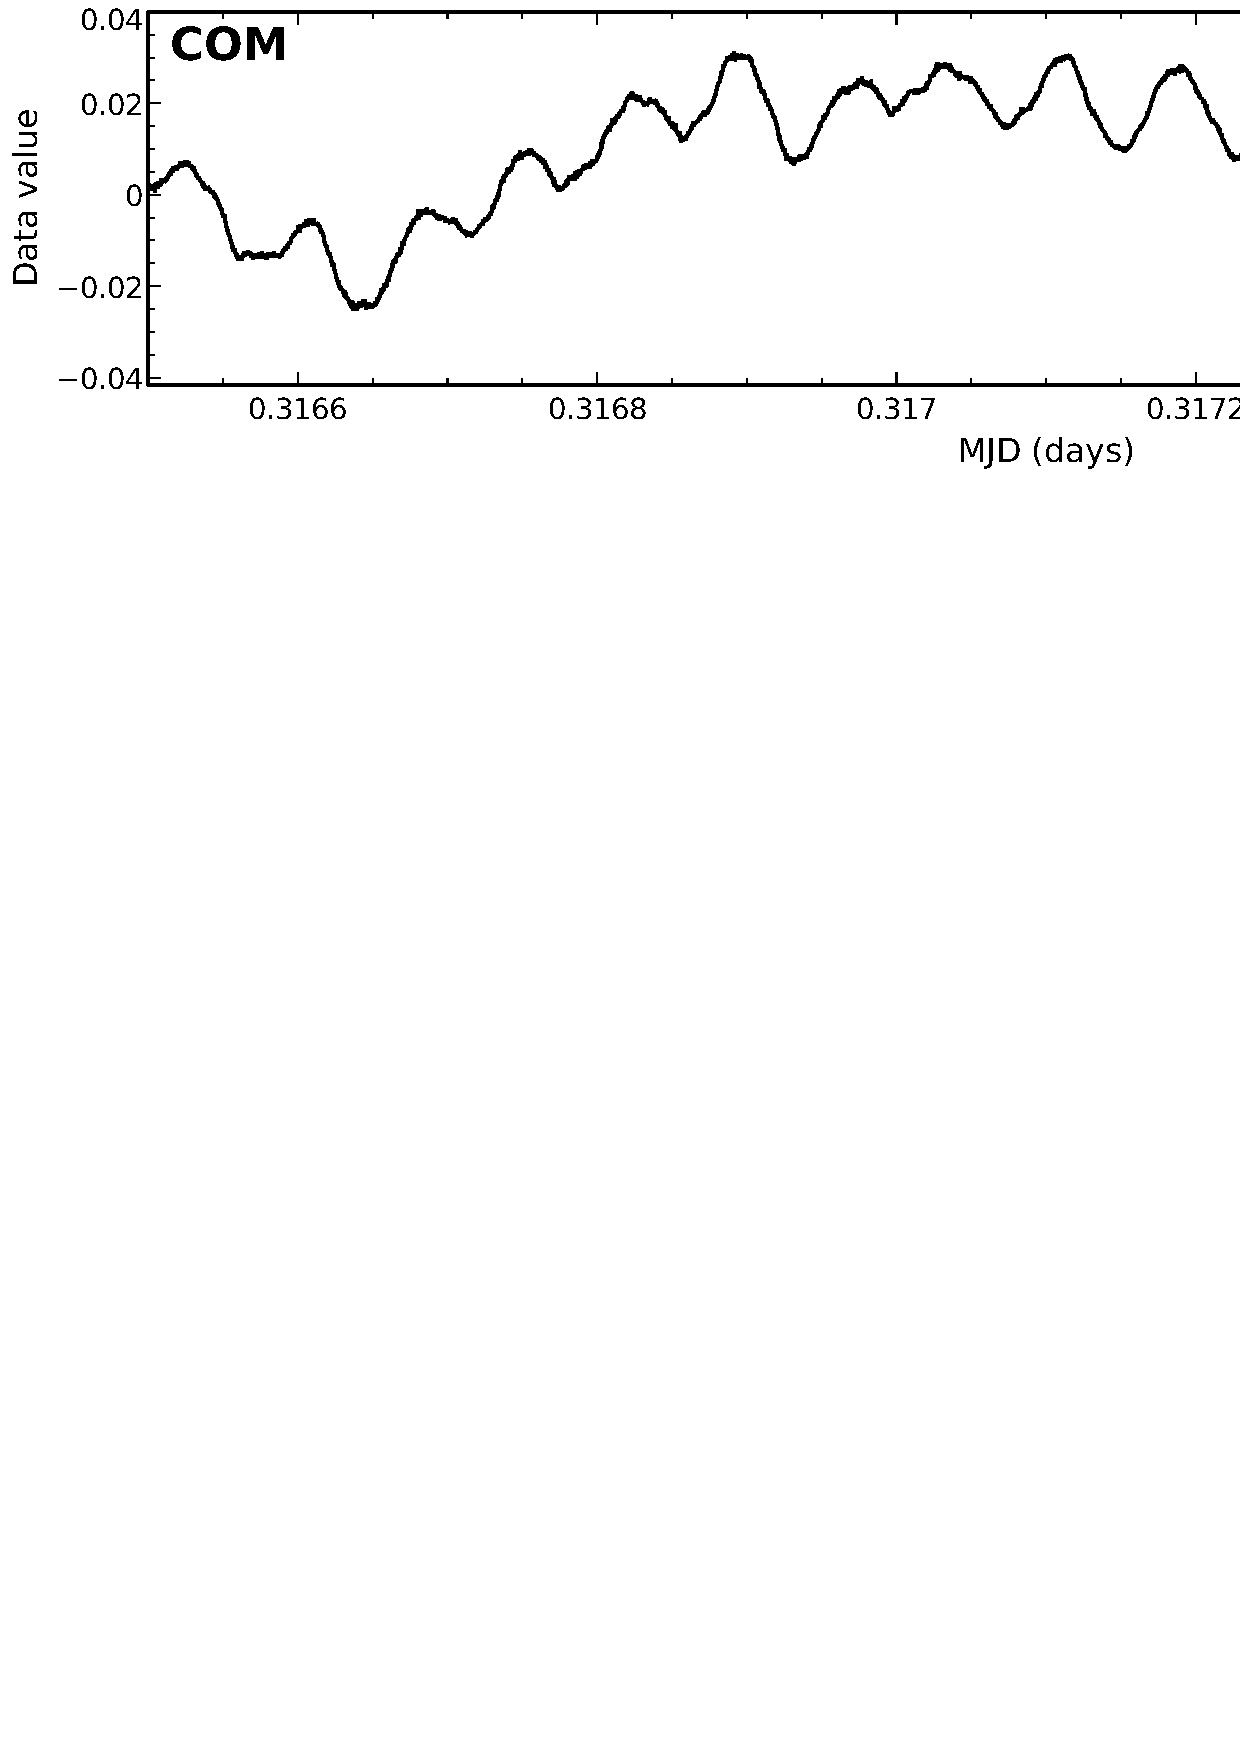
\includegraphics[width=136mm]{sc21_com} \\
  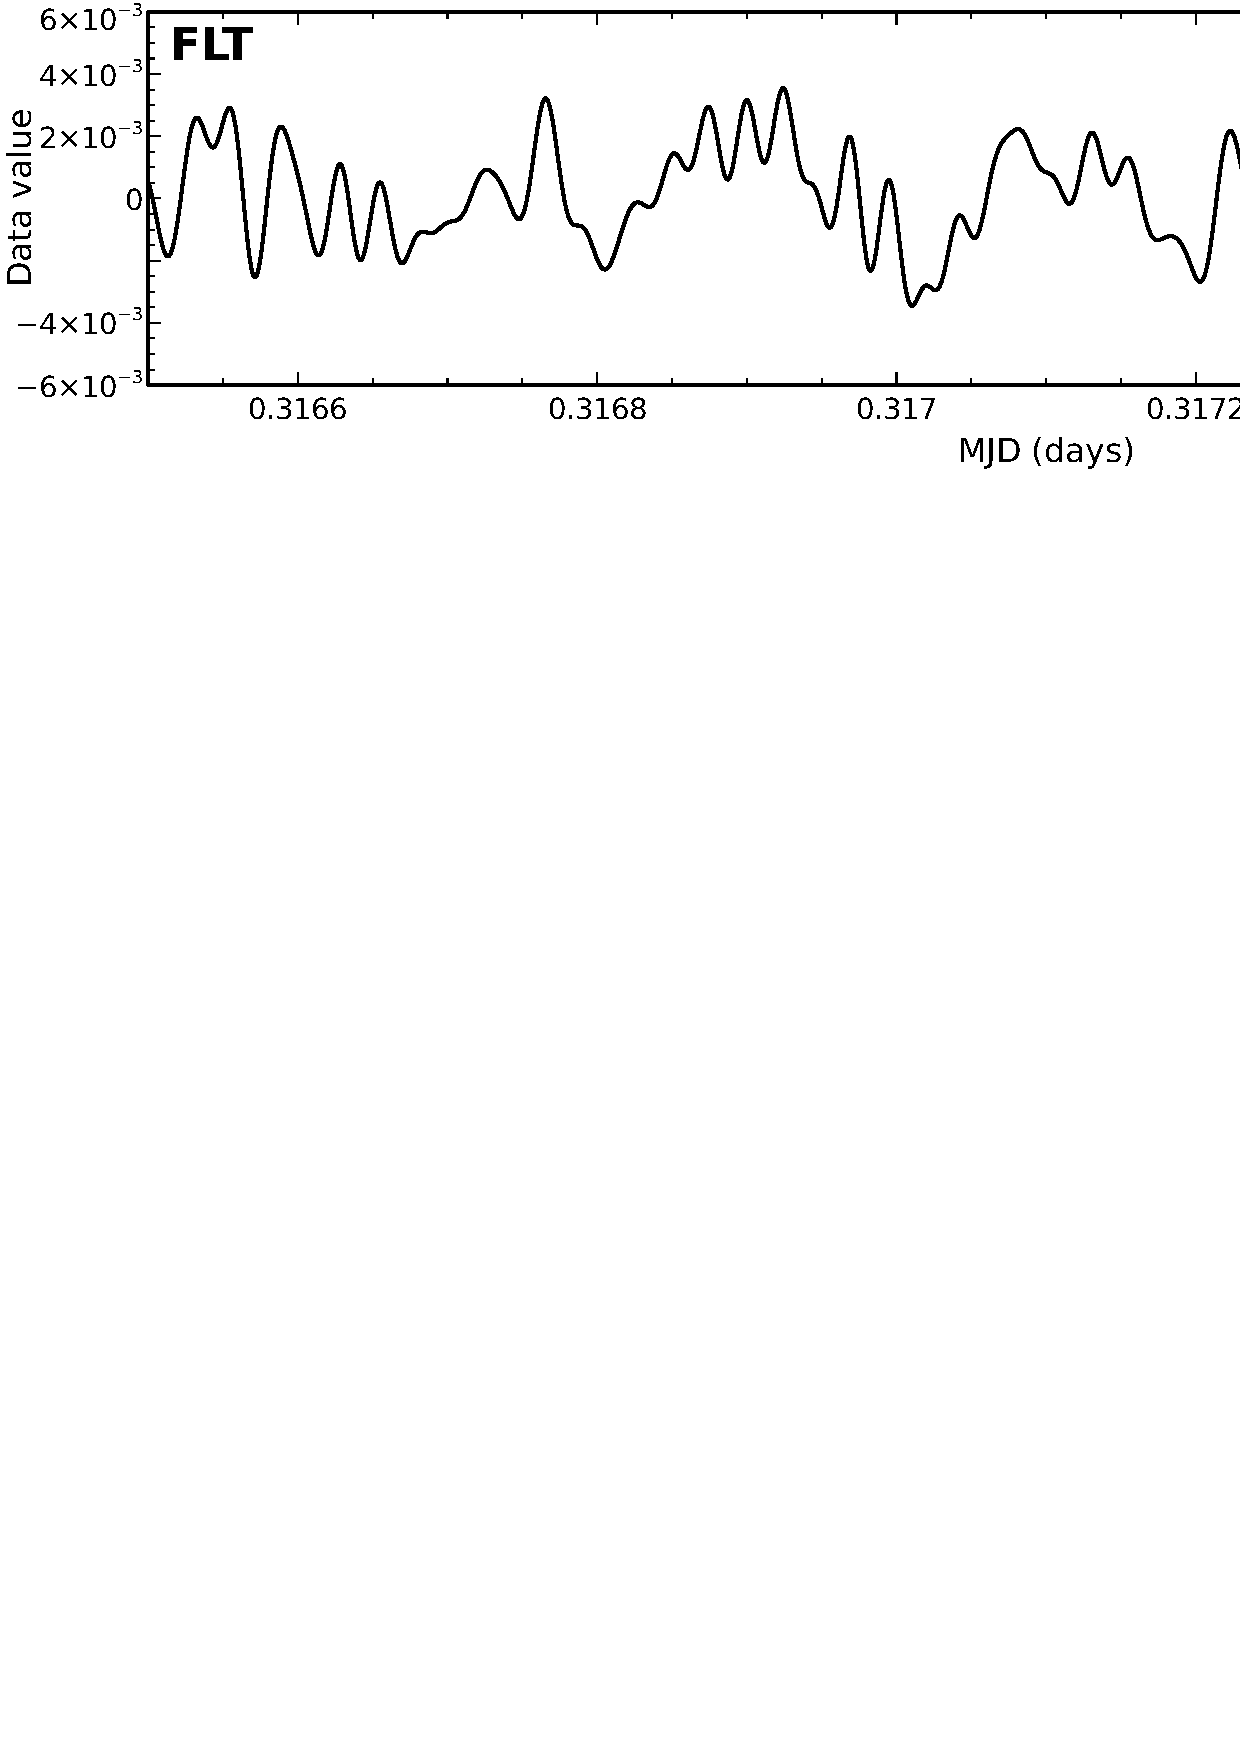
\includegraphics[width=136mm]{sc21_flt} \\
  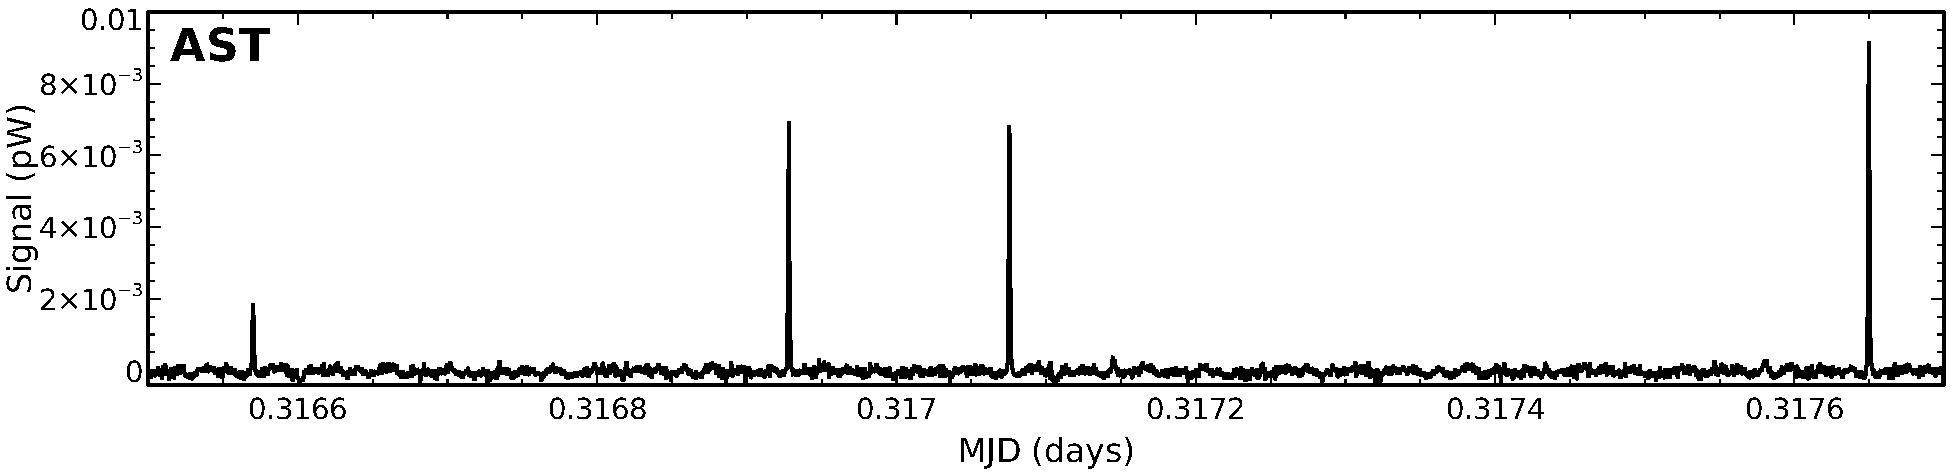
\includegraphics[width=136mm]{sc21_ast} \\
  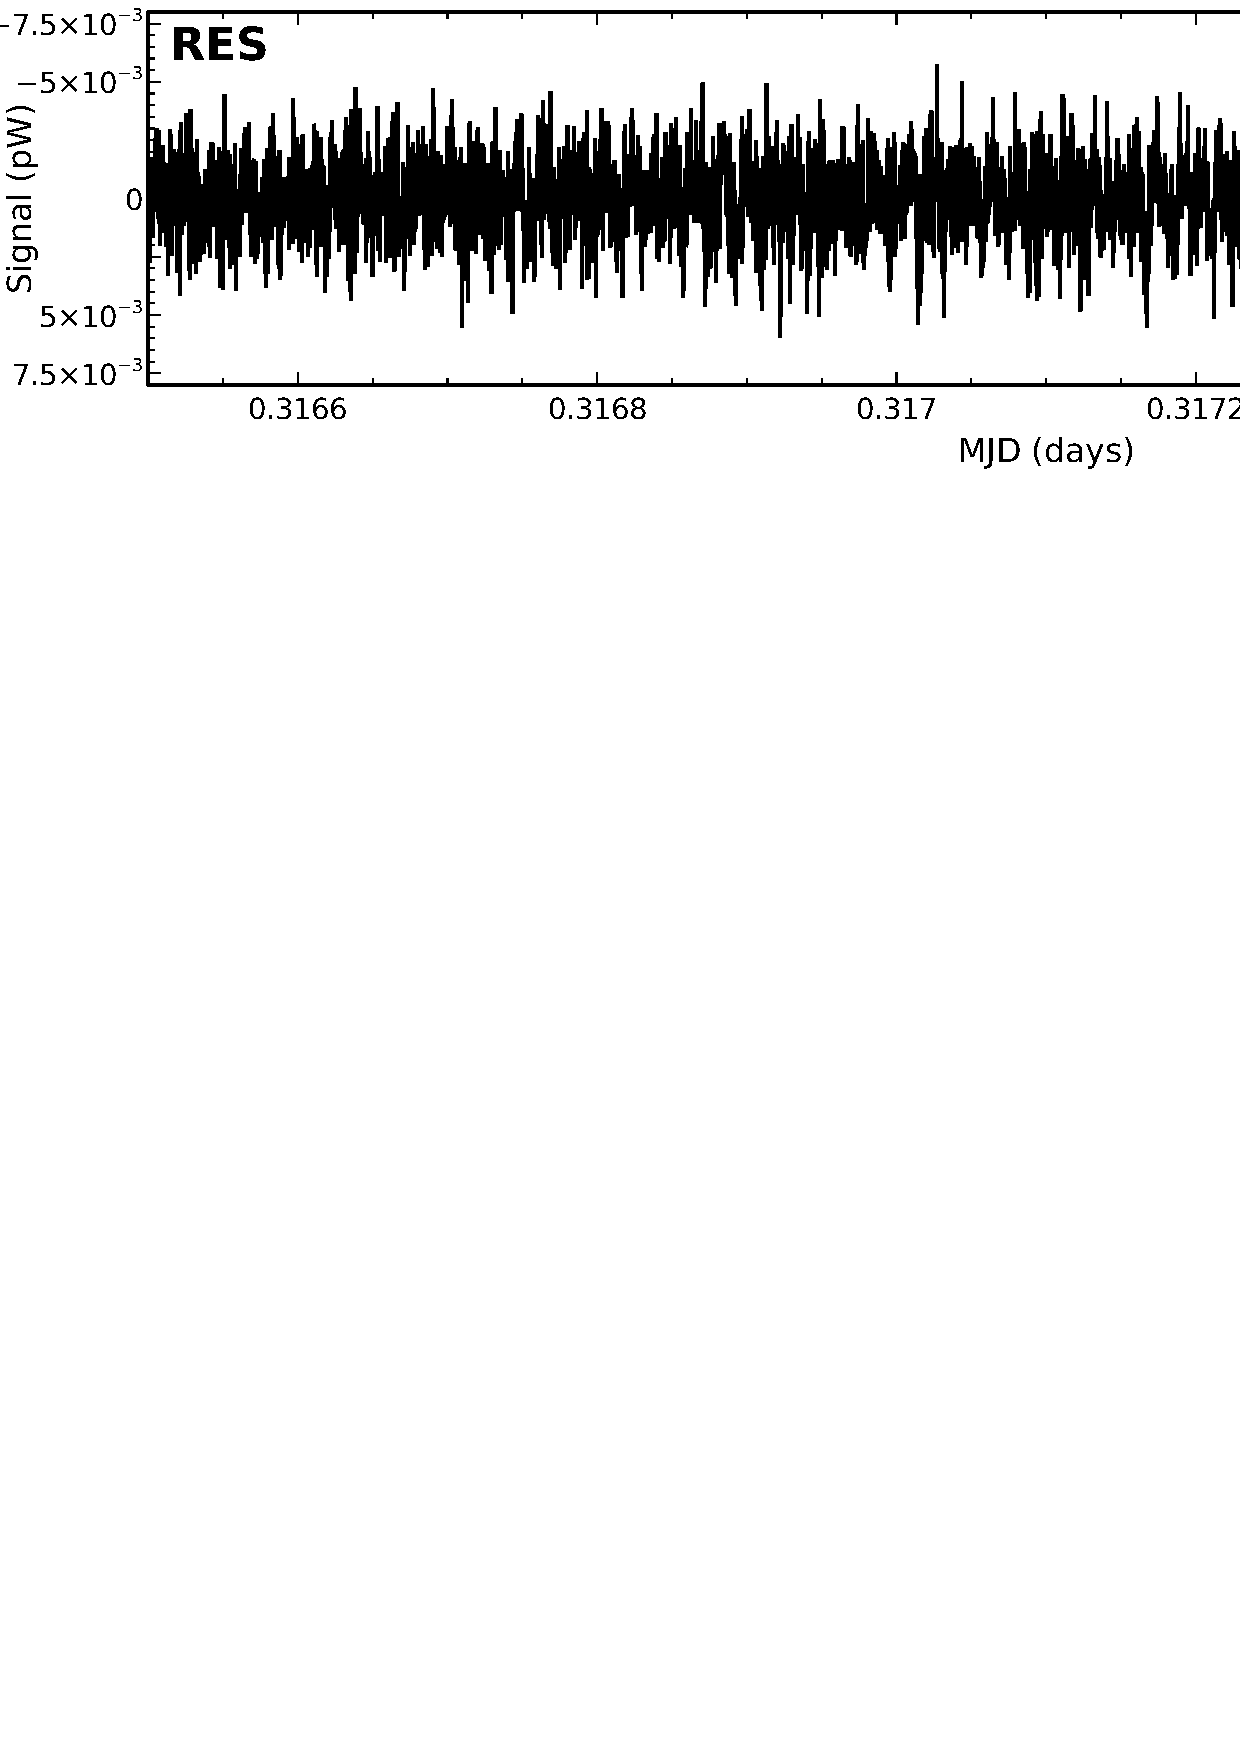
\includegraphics[width=136mm]{sc21_res} \\
\end{htmlonly}
\caption[Iterative models in the time domain]{\small Time-domain
components of the iterative models. These show the solution for the
same single bolometer for part of an observation of CRL2688. From top
to bottom: the \texttt{COM} model containing signal common to all
bolometers, the \texttt{FLT} model containing residual low-frequency
noise missed by \texttt{COM}, the \texttt{AST} model with the signal
showing as a positive spike when this bolometer passes over the
source, and the \texttt{RES} model looking (as expected) like white
noise.}
\label{fig:itercomp}
\end{center}
\end{figure}


\subsection{\xlabel{export}Exporting individual models}
\label{sec:export}

By default, the final values of these fitted models are \emph{not}
written out. However, this can be changed by setting
\texttt{exportndf} in the configuration file to the list of models
that you wish to view.
\vspace{0cm}
\begin{myquote}
\begin{verbatim}
exportndf = (com,gai,ast,flt,res,noi,qua)
\end{verbatim}
\end{myquote}

In addition to the models listed in \cref{Section}{sec:models}{The
individual models}, you request \texttt{RES} in order to export the
residual model. \texttt{RES} is the residual signal remaining after
the other models have been removed. By contrast, the \texttt{NOI}
model is the noise in \texttt{RES}, as determined by running
\texttt{RES} through \calcnoise\ (see
\cref{Section}{sec:calcnoise}{Checking the array performance}). If
\texttt{NOI} is exported, it can be viewed as the VARIANCE component
of the \texttt{RES} model; thus, export of \texttt{RES} is implied if
\texttt{NOI} is specified.


The \texttt{exportndf} parameter will write out the requested models
as NDF files with names based on the first input file that went into
the maps for each sub-array. This is first suffixed by \texttt{con},
indicating that several data files may have been concatenated
together. The three-letter code for each model is then appended to the
filename (such as \texttt{s8a20120720\_00030\_0003\_con\_com.sdf},
\begin{latexonly}
\linebreak          % \latex causes a paragraph break.
\end{latexonly}
\texttt{s8a20120720\_00030\_0003\_con\_flt.sdf},
\texttt{s8a20120720\_00030\_0003\_con\_res.sdf})\footnote{The filename shows
sub-scan 3 of Observation 30 since this is the first science file that
is encountered (see \cref{Section}{sec:raw}{Raw SCUBA-2 Data}).} The variance
and quality for the data are stored as the VARIANCE and QUALITY
components within the residual file NDF.

\begin{latexonly}
\begin{center}
\begin{fmpage}{0.95\linewidth}
\vspace{0.1cm}
TIP: You can examine any of these model components as you would the final map.
\end{fmpage}
\end{center}
\end{latexonly}

\begin{htmlonly}
\textbf{TIP: You can examine any of these model components as you would the final map.\\*\\*}
\end{htmlonly}

Examples of the time traces for a single bolometer from these output
models is shown in \cref{Figure}{fig:itercomp}{time-domain
components}. These traces cover a subset of an observation of the
secondary calibrator CRL2688. You can clearly see the dominance of the
\texttt{COM} model which is removed first. The \texttt{FLT} model
stores the data removed by the high-pass filter. In the \texttt{AST}
model, CRL2688 is clearly seen as positive spikes which appear when
the bolometer passes over the source. Finally, the residual signal
stored in \texttt{RES} is flat, indicating that most of the signal has
been successfully accounted for by the other model components.


\subsection{\xlabel{config}Specialised configuration files}
\label{sec:config}
%\hrule
%\vspace{0.2cm}
\myfig{sc21_dimmcongitree}{t}{width=\linewidth}{fig:configtree}{
  Hierarchy of the the configuration files}{
  Hierarchy of the configuration files.
}

The default configuration file \texttt{dimmconfig.lis} is intended to
provide a reasonably good map for all types of observations. However,
compromises have been made to reach that balance.

Whilst \texttt{dimmconfig.lis} is always a good recipe to start with
for your first run through of \makemap\ you will want to follow this
up with a specialised recipe that will suit your observation. A few
specialised configuration files are supplied with \smurf\ and can be
found in \texttt{\$STARLINK\_DIR/share/smurf/}.

The specialised files are all based on \texttt{dimmconfig.lis}. This
is illustrated by \cref{Figure}{fig:configtree}{figure below} where
the parameters in \texttt{dimmconfig\_bright\_extended.lis} override
any identical ones in \texttt{dimmconfig\_bright.lis} which in turn
override the values in \texttt{dimmconfig.lis}. the hierarchical
structure means the parameters at the top of the tree (or first
encountered) override any other instance of them.

Below is a description of each of the specialised configuration files.
The tables following each description list the parameters set for each
recipe. A verbatim copy of these files can be found in
\cref{Appendix}{app:special}{Specialised Configuration Files}.

\subsection{dimmconfig\_blank\_field.lis}
\begin{latexonly}
This configuration is tuned for blank field surveys for which the goal
is to detect extremely low signal-to-noise point sources.

Iteratively applying a high-pass
filter (\texttt{FLT}) can result in convergence problems when there is
little or no signal in the map. Instead, a single, harsher high-pass
filter is applied as a pre-processing step (corresponding to
200-arcsec scales at both 450\,$\mu$m and 850\,$\mu$m). There are also
more conservative cuts to remove noisy/problematic bolometers. Only 4
(positive) iterations are requested as there is no signal to confuse
to models.

The option \texttt{com.perarray}~=~1 requires the \texttt{COM} model to
be fit to each sub-array independently. This improves the overall fit
but with the loss of any structure on scales larger than a single
sub-array---not an issue for blank fields.

\cref{Figure}{fig:bfcompare}{The images below} shows the sharp
contrast in the output map between reducing data with the default
configuration file and using \texttt{dimmconfig\_blank\_field.lis}.

Blank-field maps commonly have a matched filter applied to aid source
detection (see \cref{Section}{sec:mf}{Point-source detection}),
however this is not applied by the map-maker.
\vspace{0.3cm}

\myfigduo{sc21_cosmo1-def}{sc21_cosmo1-bf}{[t!]}{width=0.47\linewidth}{fig:bfcompare}{3mm}{
  Example map reduced with \texttt{dimmconfig\_blank\_field.lis}}{
  Maps of a deep cosmology field reduced with \textbf{(left)}
  \texttt{dimmconfig.lis} and \textbf{(right)} \texttt{dimmconfig\_blank\_field.lis}.
}


% The tildes around the equal sign are to ensure HTML table field is
% not wrapped after the parameter name.
\latex{\renewcommand*\arraystretch{0.95}}
\begin{table}[h!]
\centering
\begin{tabular}{|p{6.5cm}p{7.0cm}|}
\hline
\multicolumn{2}{|l|}{\texttt{dimmconfig\_blank\_field.lis}}\\
\hline
\texttt{numiter~=~4}&\texttt{flt\_edge\_largescale~=~200}\\
\texttt{spikethresh~=~10}&\texttt{model order~=~(com,ext,ast,noi)}\\
\texttt{com.perarray~=~1}&\\
\hline
\end{tabular}
\end{table}
\end{latexonly}

\begin{htmlonly}
This configuration is tuned for blank field surveys for which the goal
is to detect extremely low signal-to-noise point sources.

Iteratively applying a high-pass
filter (\texttt{FLT}) can result in convergence problems when there is
little or no signal in the map. Instead, a single, harsher high-pass
filter is applied as a pre-processing step (corresponding to
200-arcsec scales at both 450\,$\mu$m and 850\,$\mu$m). There are also
more conservative cuts to remove noisy/problematic bolometers. Only 4
(positive) iterations are requested as there is no signal to confuse
to models.

The option \texttt{com.perarray}=1 requires the \texttt{COM} model to
be fit to each sub-array independently. This improves the overall fit
but with the loss of any structure on scales larger than a single
sub-array---not an issue for blank fields.

\cref{Figure}{fig:bfcompare}{The images below} shows the sharp
contrast in the output map between reducing data with the default
configuration file and using \texttt{dimmconfig\_blank\_field.lis}.

Blank-field maps commonly have a matched filter applied to aid source
detection (see \cref{Section}{sec:mf}{Point-source detection}),
however this is not applied by the map-maker.
\vspace{0.3cm}


% The tildes around the equal sign are to ensure HTML table field is
% not wrapped after the parameter name.
\latex{\renewcommand*\arraystretch{0.95}}
\begin{table}[h!]
\centering
\begin{tabular}{|p{6.5cm}p{7.0cm}|}
\hline
\multicolumn{2}{|l|}{\texttt{dimmconfig\_blank\_field.lis}}\\
\hline
\texttt{numiter~=~4}&\texttt{filt\_edge\_largescale~=~200}\\
\texttt{spikethresh~=~10}&\texttt{modelorder = (com,ext,ast,noi)}\\
\texttt{com.perarray~=~1}&\\
\hline
\end{tabular}
\end{table}


\myfigduo{sc21_cosmo1-def}{sc21_cosmo1-bf}{[t!]}{width=0.47\linewidth}{fig:bfcompare}{3mm}{
  Example map reduced with \texttt{dimmconfig\_blank\_field.lis}}{
  Maps of a deep cosmology field reduced with \textbf{(left)}
  \texttt{dimmconfig.lis} and \textbf{(right)} \texttt{dimmconfig\_blank\_field.lis}.
}

\end{htmlonly}


\subsection{dimmconfig\_bright\_compact.lis}

This configuration is aimed at reducing maps of bright, compact
sources that are isolated at the centre of the map (i.e. calibrators). It references
\texttt{dimmconfig\_bright.lis}, and thus the parameters from both `bright'
recipes override the default values in \texttt{dimmconfig.lis}.

The addition of \texttt{ast.zero\_circle} and
\texttt{ast.zero\_notlast} parameters are used to constrain the map to
zero beyond a radius of 1\,arcmin for all but the final iteration.
This strategy helps with map convergence significantly, and can
provide good maps of bright sources, even in cases where scan patterns
failed to complete in full.

\texttt{com.perarray} is set to 1 indicating that a \texttt{COM} model
should be fit separately for each sub-array. This is not advised for
extended sources as signal on scales larger than a single sub-array is
lost but is fine for a compact central source. Likewise, the filtering
is tighter. The S/N threshold for DC steps is relaxed from 25 in the
default file to 100 to avoid problems associated with bright sources.

% The tildes around the equal sign are to ensure HTML table field is
% not wrapped after the parameter name.
\latex{\renewcommand*\arraystretch{0.95}}
\begin{table}[h!]
\centering
\begin{tabular}{|p{6.5cm}p{7.0cm}|}
\hline
\multicolumn{2}{|l|}{\texttt{dimmconfig\_bright\_compact.lis}}\\
\hline
\texttt{numiter~=~$-$40}&\texttt{flt.filt\_edge\_largescale~=~200}\\
\texttt{com.perarray~=~1}&\texttt{flt.zero\_circle~=~(0.016666)}\\
 \texttt{ast.zero\_circle~=~(0.0166666666)}&\\
\hline
\multicolumn{2}{|l|}{\texttt{dimmconfig\_bright.lis}}\\
\hline
\texttt{noisecliphigh~=~10.0} & \texttt{dcthresh~=~100}\\
\texttt{com.corr\_tol~=~7}& \texttt{com.gain\_tol~=~7}\\
\texttt{com.gain\_abstol~=~5}& \\
\hline
\end{tabular}
\end{table}


\subsubsection{dimmconfig\_bright\_extended.lis}

\begin{latexonly}
\myfigduo{sc21_gal_def}{sc21_gal_brex}{[t!]}{width=0.47\linewidth}{fig:becompare}{3mm}{
  Example map reduced with \texttt{dimmconfig\_bright\_extended.lis}}{
  A region towards the Galactic Centre reduced with \textbf{(left)}
  \texttt{dimmconfig.lis} and \textbf{(right)}
  \texttt{dimmconfig\_bright\_extended.lis}.
}

This configuration is for reducing maps of bright extended sources,
and references \texttt{dimmconfig\_bright.lis}.  The S/N threshold for DC steps
is relaxed from \texttt{25} in the default file to \texttt{100} to
avoid problems associated with bright sources. Here
\texttt{ast.zero\_snr} is used to constrain the \texttt{AST} model to
zero wherever the S/N is lower than 5$\sigma$.  Everywhere the signal
is below this threshold, the map is set to zero for all but the final
iteration. \texttt{numiter} has been raised to \texttt{-40}, as more
iterations are required to maximise the sensitivity to large dynamic
signal ranges in the map.

Recovering both faint extended structure and bright sources in the
same field poses an extra challenge. Strategies for this are explored
in \cref{Section}{sec:tweak}{Tailoring your reduction}.

\cref{Figure}{fig:becompare}{The images below} shows a comparison between
maps reduced with the default configuration file and using
\texttt{dimmconfig\_bright\_extended.lis}; the most noticeable
difference is the improvement in the bowling around strong sources.

\latex{\renewcommand*\arraystretch{1}}
\begin{table}[h!]
\centering
\begin{tabular}{|p{6.5cm}p{6.5cm}|}
\hline
\multicolumn{2}{|l|}{\texttt{dimmconfig\_bright\_extended.lis}}\\
\hline
\texttt{numiter~=~-40}&\texttt{flt.filt\_edge\_largescale~=~480}\\
\texttt{ast.zero\_snr~=~3}&\texttt{ast.zero\_snrlo~=~2}\\
\texttt{ast.skip~=~5}&\texttt{flt.zero\_snr~=~5}\\
\texttt{flt.zero\_snrlo~=~3}& \\
\hline
\multicolumn{2}{|l|}{\texttt{dimmconfig\_bright.lis}}\\
\hline
\texttt{noisecliphigh~=~10.0} & \texttt{dcthresh~=~100}\\
\texttt{com.corr\_tol~=~7}& \texttt{com.gain\_tol~=~7}\\
\texttt{com.gain\_abstol~=~5}& \\
\hline
\end{tabular}
\end{table}
\end{latexonly}

\begin{htmlonly}
This configuration is for reducing maps of bright extended sources,
and references \texttt{dimmconfig\_bright.lis}.  The S/N threshold for DC steps
is relaxed from \texttt{25} in the default file to \texttt{100} to
avoid problems associated with bright sources. Here
\texttt{ast.zero\_snr} is used to constrain the \texttt{AST} model to
zero wherever the S/N is lower than 5$\sigma$.  Everywhere the signal
is below this threshold, the map is set to zero for all but the final
iteration. \texttt{numiter} has been raised to \texttt{-40}, as more
iterations are required to maximise the sensitivity to large dynamic
signal ranges in the map.

Recovering both faint extended structure and bright sources in the
same field poses an extra challenge. Strategies for this are explored
in \cref{Section}{sec:tweak}{Tailoring your reduction}.

\cref{Figure}{fig:becompare}{The images below} shows a comparison between
maps reduced with the default configuration file and using
\texttt{dimmconfig\_bright\_extended.lis}; the most noticeable
difference is the improvement in the bowling around strong sources.

\latex{\renewcommand*\arraystretch{1}}
\begin{table}[h!]
\centering
\begin{tabular}{|p{6.5cm}p{6.5cm}|}
\hline
\multicolumn{2}{|l|}{\texttt{dimmconfig\_bright\_extended.lis}}\\
\hline
\texttt{numiter~=~-40}&\texttt{flt.filt\_edge\_largescale~=~480}\\
\texttt{ast.zero\_snr~=~3}&\texttt{ast.zero\_snrlo~=~2}\\
\texttt{ast.skip~=~5}&\texttt{flt.zero\_snr~=~5}\\
\texttt{flt.zero\_snrlo~=~3}& \\
\hline
\multicolumn{2}{|l|}{\texttt{dimmconfig\_bright.lis}}\\
\hline
\texttt{noisecliphigh~=~10.0} & \texttt{dcthresh~=~100}\\
\texttt{com.corr\_tol~=~7}& \texttt{com.gain\_tol~=~7}\\
\texttt{com.gain\_abstol~=~5}& \\
\hline
\end{tabular}
\end{table}

\myfigduo{sc21_gal_def}{sc21_gal_brex}{[t!]}{width=0.47\linewidth}{fig:becompare}{3mm}{
  Example map reduced with \texttt{dimmconfig\_bright\_extended.lis}}{
  A region towards the Galactic Centre reduced with \textbf{(left)} \texttt{dimmconfig.lis}
  and \textbf{(right)} \texttt{dimmconfig\_bright\_extended.lis}.
}
\end{htmlonly}

\subsubsection{Problem solving configuration files}

Two trouble-shooting configuration files are available to supplement
dimmconfig\_bright\_extended:

\texttt{dimmconfig\_fix\_convergence} to help your map converge\\*
\texttt{dimmconfig\_fix\_blobs} to remove large blooms or blobs of
spurious emission in your final map.

The point to dimmconfig\_bright\_extended.lis so the parameters are in
addition to those listed above. These files are discussed in more
detail in chapter \ref{sec:tweak}.

\clearpage

\section{\xlabel{maps}Reducing your Data}
\label{sec:maps}

This chapter describes how to run the map-maker and what to look out
for during processing. We also discuss reducing your data using the
\oracdr\ science pipeline and why you might want to chose this option.

As discussed in \cref{Section}{sec:dimm}{The
Dynamic Iterative Map-Maker}, all of the settings for the map-maker
are stored in configuration files. In this chapter we use
the default configuration file, \texttt{dimmconfig.lis} to reduce CRL2688,
one of SCUBA-2's secondary calibrators. For an
overview of the specialised configuration files available see
\cref{Section}{sec:config}{this section}.

\subsection{\xlabel{running_dimm}Running the iterative map-maker}
\label{sec:running}

When running the map-maker, you can call any of the provided
configuration files directly from the Starlink path (e.g.
\texttt{\^\$STARLINK\_DIR/share/smurf/dimmconfig.lis}). Alternatively,
a local copy can be made and edited. Advice on which parameters to
edit can be found in \cref{Section}{sec:tweak}{Tweaking the
configuration file}.

\begin{latexonly}
\begin{center}
\begin{fmpage}{0.95\linewidth}
\vspace{0.1cm}
TIP: An up-caret (\,\^\,) is required any time you are reading in
a  text file in \starlink. For the map-maker this includes the
configuration file and a list of your input files (e.g. \texttt{in=\^\,myrawfiles.txt}).
\end{fmpage}
\end{center}
\end{latexonly}

\begin{htmlonly}
\textbf{TIP: An up-caret (\,\^\,) is required any time you are reading in
a  text file in \starlink. For the map-maker this includes the
configuration file and a list of your input files (e.g. \texttt{in=\^\,myrawfiles.txt}).\\*\\*}
\end{htmlonly}

The default pixel sizes are:

2\,arcsec at 450$\mu$m\\
4\,arcsec at 850$\mu$m

These can be changed by adding the \texttt{pixsize=}$x$ to the
command string\footnote{The default sizes are defined as one quarter
of the Airy disk rounded up to the nearest half arcsecond.}, where $x$
is your desired pixel size in arcseconds. We advise that you do not
increase the pixel size at this stage as it will compromise model
fitting---instead regrid your map as a post-processing step.

%Other ADAM parameter available with \makemap\ include ref, maxmem and
%msg\_filter. Some of these appear in the example below but see
%\cref{Appendix}{app:adam}{MAKEMAP ADAM Parameters} for descriptions. A
%complete list of all ADAM parameters can be found in \smurfsun.

\begin{latexonly}
\begin{center}
\begin{fmpage}{0.95\linewidth}
\vspace{0.1cm}
TIP: Map-maker not finding your raw files from a path? Check you have
double quotes around your `in' option and are not using *sdf---use
either *.sdf or just *.
\end{fmpage}
\end{center}
\end{latexonly}

\begin{htmlonly}
\textbf{TIP: Map-maker not finding your raw files from a path? Check
you have double quotes around your `in' option and are not using
*sdf---use either *.sdf or just *.\\*\\*}
\end{htmlonly}


\begin{myquote}
\begin{verbatim}
% makemap in="/jcmtdata/raw/scuba2/s8*/20120720/00030/*.sdf" out=850_crl2688 \
  config=^$STARLINK_DIR/share/smurf/dimmconfig.lis


Out of 32 input files, 4 were darks, 8 were fast flats and 20 were science
Processing data from instrument 'SCUBA-2' for object 'CRL2688' from the
following observation  :
  20120720 #30 scan  /shutter

MAKEMAP: Map-maker will use no more than 68401 MiB of memory

Projection parameters used:
CRPIX1 = 0
CRPIX2 = 0
CRVAL1 = 315.578333333333 ( RA = 21:02:18.800 )
CRVAL2 = 36.6938055555556 ( Dec = 36:41:37.70 )
CDELT1 = -0.00111111111111111 ( -4 arcsec )
CDELT2 = 0.00111111111111111 ( 4 arcsec )
CROTA2 = 0

Output map pixel bounds: ( -132:122, -126:129 )

Output map WCS bounds:
Right ascension: 21:01:38.318 -> 21:03:03.280
Declination: 36:33:07.19 -> 36:50:11.70

smf_iteratemap: will down-sample data to match angular scale of 4 arcsec
smf_iteratemap: Iterate to convergence (max 5)
smf_iteratemap: stop when change in chi^2 < 0.001
smf_iteratemap: provided data are in 1 continuous chunks, the largest of which
has 5957 samples (153.729 s)
smf_iteratemap: map-making requires 1376 MiB (map=3 MiB model calc=1372 MiB)
smf_iteratemap: Continuous chunk 1 / 1 =========
smf_calc_smoothedwvm: 0.977444 s to calculate unsmoothed WVM tau values
smf_iteratemap: Iteration 1 / 5 ---------------
--- Size of the entire data array ------------------------------------------
bolos  : 5120
tslices: bnd:0(0.0 min), map:5957(2.6 min), tot:5957(2.6 min)
Total samples: 30499840
--- Quality flagging statistics --------------------------------------------
 BADDA:   10972794 (35.98%),        1842 bolos
BADBOL:   11818688 (38.75%),        1984 bolos
DCJUMP:      38809 ( 0.13%),
  STAT:      71680 ( 0.24%),          14 tslices
 NOISE:     810152 ( 2.66%),         136 bolos
Total samples available for map:   18634826, 61.10% of max (3128.22 bolos)
smf_iteratemap: Calculate time-stream model components
smf_iteratemap: Rebin residual to estimate MAP
smf_iteratemap: Calculate ast
--- Quality flagging statistics --------------------------------------------
 BADDA:   10972794 (35.98%),        1842 bolos  ,change          0 (+0.00%)
BADBOL:   11925914 (39.10%),        2002 bolos  ,change     107226 (+0.91%)
DCJUMP:      38809 ( 0.13%),                    ,change          0 (+0.00%)
  STAT:      71680 ( 0.24%),          14 tslices,change          0 (+0.00%)
   COM:     323165 ( 1.06%),                    ,change     323165 (+0.00%)
 NOISE:     810152 ( 2.66%),         136 bolos  ,change          0 (+0.00%)
Total samples available for map:   18312771, 60.04% of max (3074.16 bolos)
     Change from last report:    -322055, -1.73% of previous
smf_iteratemap: Will calculate chi^2 next iteration
smf_iteratemap: *** NORMALIZED MAP CHANGE: 0.874979 (mean) 73.7106 (max)
smf_iteratemap: Iteration 2 / 5 ---------------
smf_iteratemap: Calculate time-stream model components
smf_iteratemap: Rebin residual to estimate MAP
smf_iteratemap: Calculate ast
--- Quality flagging statistics --------------------------------------------
 BADDA:   10972794 (35.98%),        1842 bolos  ,change          0 (+0.00%)
BADBOL:   11949742 (39.18%),        2006 bolos  ,change      23828 (+0.20%)
 SPIKE:         34 ( 0.00%),                    ,change         34 (+0.00%)
DCJUMP:      38809 ( 0.13%),                    ,change          0 (+0.00%)
  STAT:      71680 ( 0.24%),          14 tslices,change          0 (+0.00%)
   COM:     357816 ( 1.17%),                    ,change      34651 (+10.72%)
 NOISE:     810152 ( 2.66%),         136 bolos  ,change          0 (+0.00%)
Total samples available for map:   18278374, 59.93% of max (3068.39 bolos)
     Change from last report:     -34397, -0.19% of previous
smf_iteratemap: *** CHISQUARED = 0.983228126551834
smf_iteratemap: *** NORMALIZED MAP CHANGE: 1.29181 (mean) 15.0552 (max)
smf_iteratemap: Iteration 3 / 5 ---------------
.....
.....
.....
smf_iteratemap: Iteration 5 / 5 ---------------
smf_iteratemap: Calculate time-stream model components
smf_iteratemap: Rebin residual to estimate MAP
smf_iteratemap: Calculate ast
--- Quality flagging statistics --------------------------------------------
 BADDA:   10972794 (35.98%),        1842 bolos  ,change          0 (+0.00%)
BADBOL:   11949742 (39.18%),        2006 bolos  ,change          0 (+0.00%)
 SPIKE:         34 ( 0.00%),                    ,change          0 (+0.00%)
DCJUMP:      38809 ( 0.13%),                    ,change          0 (+0.00%)
  STAT:      71680 ( 0.24%),          14 tslices,change          0 (+0.00%)
   COM:     362902 ( 1.19%),                    ,change          0 (+0.00%)
 NOISE:     810152 ( 2.66%),         136 bolos  ,change          0 (+0.00%)
Total samples available for map:   18273302, 59.91% of max (3067.53 bolos)
     Change from last report:          0, +0.00% of previous
smf_iteratemap: *** CHISQUARED = 0.952708604771402
smf_iteratemap: *** change: -0.000109049487216351
smf_iteratemap: *** NORMALIZED MAP CHANGE: 0.107427 (mean) 2.96138 (max)
smf_iteratemap: ****** Completed in 5 iterations
smf_iteratemap: ****** Solution CONVERGED
Total samples available from all chunks: 18273302 (3067.53 bolos)
\end{verbatim}
\end{myquote}
%\vspace{-10mm}
%\begin{center}
%\latex{\line(1,0){155}}
%\end{center}
\begin{htmlonly}
\myfig{sc21_crl2688}{[t!]}{width=0.7\linewidth}{fig:itermap}{
  CRL2688 produced with \makemap}{
  Map of CRL2688 produced with the \smurf\ task \makemap\ using the
  iterative algorithm with default parameters.
}
\end{htmlonly}

\subsection{\xlabel{look_for}What to look out for}
%\flushbottom

Once the map-maker has completed you can open your output map using
\gaia---see \cref{Figure}{fig:itermap}{this example}. The excerpt
in \cref{Section}{sec:running}{Running the iterative map-maker} shows
the output written to the terminal as you run the map-maker. There are
a number of clues in this output that indicate the status of the
reduction.
\begin{latexonly}
\myfig{sc21_crl2688}{[t!]}{width=0.7\linewidth}{fig:itermap}{
  CRL2688 produced with \makemap}{
  Map of CRL2688 produced with the \smurf\ task \makemap\ using the
  iterative algorithm with default parameters.
}
\end{latexonly}
\\*\\*
\textbf{The number of input files}\\
The first to note is the number of input files; it is worth checking
this matches your expected number. Also summarised are the source
name, UT date and scan number.
\\*\\*
\textbf{Map dimensions}\\
Next the basic dimensions of the data being processed are listed near
the start of the first iteration. The example above has 4\,arcsec
pixels---the default at 850$\mu$m.
\\*\\*
\textbf{Chunking}\label{box:chunk}\\
The map-maker then determines if the raw data should be split and
processed in more than one chunk. In this map the data is reduced in
one continuous piece: \param{Continuous chunk 1 / 1}. Chunking is
where the map-maker processes sub-sections of the time-series data
independently and should be avoided if possible---see the text box
below.
\html{\newline}

% The minipages used for the dvi version give latex2html problems.
\begin{htmlonly}
\htmladdimg{sc21_data_chunking.png}
\newline\newline
\end{htmlonly}

\begin{latexonly}
\colorbox{gray}{
\label{page:text}
\hspace{0.1cm}
\begin{minipage}[t]{0.93\linewidth}
\vspace{0.2cm}

\textbf{Data Chunking}\\
Chunking occurs when there is insufficient computer memory available
for the map-maker or when there is a gap in the time-series data (e.g.
from a missing sub-scan). In these cases, the map-maker divides up the
time-series data and reduces each sub-portion independently, before
re-combining all the outputs at a later stage. Ideally you want your
data reduced in a single chunk, however this can be unfeasible for
large maps.
\vspace{0.2cm}\\
The more data the map-maker processes at once, the better chance it
has of determining the difference between sky signal and background
noise. In \textsc{daisy} mode chunking is less of a concern as
the entire map area is covered many times in the space of a single
observation.
\vspace{0.2cm}\\
For \textsc{pong} maps chunking is a bigger concern, with the
maximum number of chunks that can be tolerated dependent on the number
of map rotations. For example, a 40-minute \textsc{pong} map with eight
rotations may get divided into three or four chunks. Although not
ideal, this will mean that each point is still covered by two or three
passes. Fewer passes than this however and the map-maker become less
effective.
\vspace{0.2cm}
\end{minipage}
\hspace{0.1cm}
}
\end{latexonly}
\latex{\newline\newline}

\textbf{Quality statistics}\\
At the beginning of the reduction, the main purpose of QUALITY
flagging is to indicate how many bolometers are being used. In the
example above you can see that from a total of 5120 bolometers, 1842
were turned off during data acquisition (\texttt{BADDA}). In addition,
136 bolometers
exceeded the acceptable noise threshold (\texttt{NOISE}), while tiny
fractions of the data were flagged because the telescope was moving
too slowly (\texttt{STAT}) or the sample are adjacent to a step that
was removed (\texttt{DCJUMP}).

The total number of bad bolometers (\texttt{BADBOL}) is 1984.
Accounting for these, and the small numbers of additionally flagged
samples, 3128.22 effective bolometers are available after initial
cleaning\footnote{The fractional number is due to time-slices being
removed during cleaning. The number of bolometers is then
reconstructed from the number of remaining time-slices}.

After each subsequent iteration a new `Quality' report is produced,
indicating how the flags have changed. An important flag that appears
in the `Quality' report following the first iteration is \texttt{COM}:
the DIMM rejects bolometers (or portions of their time series) if they
differ significantly from the common-mode (average) of the remaining
bolometers.

You may note that compared with the initial report, the total number of samples
with good `Quality' (\texttt{Total samples available for map}) has
dropped from 18634826 to 18273302 (about a 2 per cent decrease) as
additional samples were flagged in each iteration.

Be aware that some large reductions may take many iterations to reach
convergence and you may find significantly fewer bolometers remaining
resulting in higher noise than expected.

\textbf{Convergence}\\
The convergence criteria \texttt{maptol} is updated for each
iteration. The convergence can be checked from the line reporting\\*
\hspace*{0.5cm} \texttt{smf\_iteratemap: *** NORMALIZED MAP CHANGE:
0.10559 (mean) 2.81081 (max)}

The number to look out for is the mean value. This will have to drop
below your required \texttt{maptol} for convergence to be achieved.

The default configuration file used in this example executes a maximum
of five iterations, but stops sooner if the change in \texttt{maptol}
drops below 0.05 (i.e. \texttt{numiter~=$-$5}). In this example it
stops after five iterations:

\begin{latexonly}
\begin{center}
\begin{fmpage}{0.95\linewidth}
\vspace{0.1cm}
TIP: You can interrupt the processing at any stage with a
single \texttt{Ctrl-C}. The map-maker will complete the iteration then write
out a final science map. Entering \texttt{Ctrl-C} twice will
kill the process immediately.
\end{fmpage}
\end{center}
\end{latexonly}

\begin{htmlonly}
\textbf{TIP: You can interrupt the processing at any stage with a
single \texttt{Ctrl-C}. The map-maker will complete the iteration then write
out a final science map. Entering \texttt{Ctrl-C} twice  will
kill the process immediately.\\*\\*}
\end{htmlonly}

\subsection{\xlabel{sciencepl}Using the science pipeline}

You can also reduce your data using the \oracdr\ science pipeline on a
local computer. There are advantages to running the map-maker using
the pipeline. You can feed the pipeline observations of multiple
sources rather than feed in a single source at a time. The pipeline
will recognise the different sources and make a separate map for each,
whereas the map-maker would make a single large map that would include
all your sources (no matter how widely spaced!).

Another useful feature is that the pipeline will generate a log files to record
various useful quantities. The standard log files from reducing
science data are:

\begin{itemize}
\item \texttt{log.noise}---noise in the map for each observation and the co-add
(calculated from median of error component)
\item \texttt{log.nefd}---NEFD calculated for each observation and for the co-added map(s)
\end{itemize}
The pipeline will produce calibrated maps; by default these are
calibrated using the standard FCFs, although users can specify their
own if they wish.

Running the science pipeline is very straightforward and can be as
simple as the example below. Here a list is made of all your raw data,
the pipeline is then initiated, finally the reduction is started with
instructions to loop through all data listed in the supplied file and
the filename in question is given.

\begin{myquote}
\begin{verbatim}
% ls s8*.sdf > myfiles.lis
% oracdr_scuba2_850
% oracdr -loop file -files myfiles.lis
\end{verbatim}
\end{myquote}

\textbf{For a more in-depth discussion on running the pipeline and a discussion
of the various outputs see \cref{Section}{sec:pipe}{The SCUBA-2
Pipeline} or \pipelinesun.}
\clearpage


\section{\xlabel{postprocess}Post-processing Reduction Steps}
\label{sec:postprocess}

\subsection{\xlabel{apply_fcf}Flux Conversion Factors (FCFs)}
\label{sec:cmult}

When your data comes out of the map-maker it is in units of picowatts
(pW). A flux conversion factor, or FCF, needs to be applied to scale
your data from units of pW to janskys (Jy). For more information on calibrating
SCUBA-2 data see Dempsey et al. (2013) \cite{dempsey12}.
\\*\\*
Below are our default FCFs. Note that the \fcfb\ will be applied
by the pipeline when reducing your data with \oracdr.

\vspace{0.5cm}
\renewcommand*\arraystretch{1.2}
\begin{table}[h!]
\centering
\begin{tabular}{|c|c|c|c|}
\hline
\multicolumn{2}{|c|}{\textbf{APERTURE}}  &
\multicolumn{2}{c|}{\textbf{PEAK}}      \\
\hline
\multicolumn{2}{|c|}{\fcfa\ (Jy/pW/arcsec$^2$) }  &
\multicolumn{2}{c|}{\fcfb\ (Jy/pW/beam)}      \\
\hline
\hspace{0.4cm} 450\,$\mu$m \hspace{0.3cm} & 850\,$\mu$m & \hspace{0.4cm} 450\,$\mu$m \hspace{0.3cm}& 850\,$\mu$m \\
\hline
4.71 $\pm$ 0.5& 2.34 $\pm$ 0.08& 491 $\pm$ 67& 537 $\pm$ 24 \\
\hline
\end{tabular}
\end{table}
\renewcommand*\arraystretch{1.0}
\vspace{0.5cm}

\textbf{IMPORTANT NOTES:
  \newline
  (1) The standard FCF to be applied depends on
  the reduction date for your data. For data that have been
  \emph{reduced prior} to July 2012 you should see
  \cref{Appendix}{app:fcfs}{FCFs by Reduction Date} for alternative FCFs.
  \newline
  (2) Due to a glitch in the WVM, data reduced between 2012 Sept. 19,
  and 2013 Jan. 18 must be re-reduced using the latest version of
  Starlink (Hikianalia or later), or should have an FCF derived from a
  calibrator reduced at the same time (and not our standard FCF) applied
  to it.
}

\subsubsection{Aperture flux}

To get the flux density of extended sources with aperture
photometry you should apply the \fcfa.  You can then sum the emission
in an aperture. \fcfa\ was determined using a 60-arcsec diameter
aperture. If your aperture differs from this you should scale your
flux accordingly---the scaling factor can be read off the curve of
growth (see \cref{Appendix}{app:cog}{this appendix}). This graph gives
the ratio of aperture flux to total flux for a range of aperture diameters.

\fcfa\ is determined using 1\,arcsec pixels. For different pixel sizes
you will also need to apply a factor of pixelsize squared.

\subsubsection{Peak flux}

If you want to read off the peak flux from your map, you should apply
the \fcfb\ (also known as the peak FCF).  When you open your map in
\gaia\ the value of the brightest pixel will be the peak flux of your
source. (If your source is point-like, the peak value in the map is
the total flux density). Applying \fcfb\ will result in a map with
units of Jy/beam. For point-like or compact sources smaller than the
beam (with a Gaussian profile), this peak value will be the flux
density of your source.

\subsubsection{Determining your own FCF}

Calibration observations are taken at various points throughout the
night and we recommend you compare the FCF calculated from your
nearest calibrator to the standard FCF. You can use this FCF to scale
the the standard value accordingly. You should chose the calibrator
nearest in time to your science observations, unless the weather has
changed significantly.

\vspace{1mm}
\begin{minipage}[t]{0.05\linewidth}
\texttt{(1)}
\end{minipage}
\begin{minipage}[t]{0.95\linewidth}
Reduce the calibrator with the map-maker using
\texttt{dimmconfig\_bright\_compact.lis} as the configuration file.
\end{minipage}
\vspace{1mm}\\
\begin{minipage}[t]{0.05\linewidth}
\texttt{(2)}
\end{minipage}
\begin{minipage}[t]{0.95\linewidth}
Determine the FCF value by passing the output map to the
\picard\ recipe \xref{\drrecipe{SCUBA2\_CHECK\_CAL}}{sun265}{SCUBA2_CHECK_CAL}.
\begin{myquote}
\begin{verbatim}
% picard SCUBA2_CHECK_CAL 850calibrator.sdf
\end{verbatim}
\end{myquote}
This will produce a log file (\texttt{log.checkcal}) which records the both
\fcfb\ and \fcfa. Check that these values closely approximate the
standard FCF values given above.
\end{minipage}
\vspace{1mm}\\
\begin{minipage}[t]{0.05\linewidth}
\texttt{(3)}
\end{minipage}
\begin{minipage}[t]{0.95\linewidth}
Re-reduce the calibrator using the map-maker with the \emph{same}
configuration file you used for your science observations.
\end{minipage}
\vspace{1mm}\\
\begin{minipage}[t]{0.05\linewidth}
\texttt{(4)}
\end{minipage}
\begin{minipage}[t]{0.95\linewidth}
Again determine the FCF using \drrecipe{SCUBA2\_CHECK\_CAL}.
\end{minipage}
\vspace{1mm}\\
\begin{minipage}[t]{0.05\linewidth}
\texttt{(5)}
\end{minipage}
\begin{minipage}[t]{0.95\linewidth}
Apply this FCF to your reduced science data using \cmult-- see next
section. Remember to apply the pixel size squared factor if using
\fcfa.
\end{minipage}

\subsubsection{Applying the FCF}

You can apply the FCF using the \picard\ recipe
\xref{\drrecipe{CALIBRATE\_SCUBA2\_DATA}}{sun265}{CALIBRATE\_SCUBA2\_DATA}.
By default this will multiply your map by
1000$\times$\fcfb\ from the start of
\cref{Section}{sec:cmult}{Flux Conversion Factors}. This produces a
calibrated map with units of mJy/beam.

You can supply a parameter file if you wish to use a different value
for the FCF or use \fcfa. The recipe will write out the calibrated
file with an \texttt{\_cal} suffix and will change the units in the
map header.

\begin{myquote}
\begin{verbatim}
% picard CALIBRATE_SCUBA2_DATA  mapinpW.sdf
\end{verbatim}
\end{myquote}
Note that the recipe will also take account of the pixel size when
applying \fcfa.


\subsection{\xlabel{crop}Cropping your map}
\label{sec:crop}

The nature of the scan patterns results in SCUBA-2 maps significantly
larger than the requested size. The high noise towards the outer edges
is a consequence of the scanning pattern. Although this excess data is
down-weighted during reduction by the map-maker, you may wish to remove
it before either combining maps (see
\cref{Section}{sec:coadd}{Co-adding multiple maps}) or publishing your
map.

You can crop your map to the map-size set in the data header or
to any requested size of box or circle using the \picard\ recipe
\xref{\drrecipe{CROP\_JCMT\_IMAGES}}{sun265}{CROP\_JCMT\_IMAGES}.
The centre of the cropping area will always be the centre of your map.
\begin{myquote}
\begin{verbatim}
% picard -recpars mypar.lis CROP_JCMT_IMAGES map_cal.sdf
\end{verbatim}
\end{myquote}
The example above includes a parameter file specifying the radius of
the circle to be extracted (in arcsecs).  The format for the parameter
file is shown below.
\begin{center}
\begin{myquote}
\begin{verbatim}
[CROP_JCMT_IMAGES]
MAP_RADIUS = 1800.0
\end{verbatim}
\end{myquote}
\end{center}

If this parameter file is omitted it will default to a box of sides
equal to the map size in the header (as requested in the MSB). The
output from \drrecipe{CROP\_JCMT\_IMAGES} is a file with the suffix
\texttt{\_crop}. Full details of this recipe can be found in the
\htmladdnormallink{\textsc{Picard}
website}{http://www.oracdr.org/oracdr/PICARD}\latex{\footnote{http://www.oracdr.org/oracdr/PICARD}}.

\begin{latexonly}
\begin{center}
\begin{fmpage}{0.95\linewidth}
\vspace{0.1cm}
TIP: The default crop shape will be a square. Avoid losing good data
by specifying a circle using the parameter file.
\end{fmpage}
\end{center}
\end{latexonly}

\begin{htmlonly}
\textbf{TIP: The default crop shape will be a square. Avoid losing
good data by specifying a circle using the parameter file.\\*\\*}
\end{htmlonly}


\subsection{\xlabel{coadd}Co-adding multiple maps}
\label{sec:coadd}

You may have multiple maps of the same source which you would like to
co-add. \picard\ has a recipe called
\xref{\drrecipe{MOSAIC\_JCMT\_IMAGES}}{sun265}{MOSAIC_JCMT_IMAGES}
that co-adds maps while correctly dealing with the exposure time and
weights NDF extensions.
\begin{myquote}
\begin{verbatim}
% picard -recpars mypar.lis MOSAIC_JCMT_IMAGES 850map*_cal_crop.sdf
\end{verbatim}
\end{myquote}
This creates a single output file based on the name of the last file
in the list, and with a suffix \texttt{\_mos}.

There are a number of options associated with
\drrecipe{MOSAIC\_JCMT\_IMAGES} (see the \textsc{Picard} manual for a full
description). However, the main one is choosing between \wcsmosaic\
(default) and the \ccdpack\ option \makemos\ for the combination
method. For more information on \task{makemos} and advice on choosing the
best method see \xref{\textbf{SUN/139}}{sun139}{}.

An example parameter file like the one below chooses \task{makemos}
using a 3-$\sigma$ clipping threshold.

\begin{myquote}
\begin{verbatim}
[MOSAIC_JCMT_IMAGES]
MOSAIC_TASK = makemos
MAKEMOS_METHOD = sigmas
MAKEMOS_SIGMAS = 3
\end{verbatim}
\end{myquote}

Currently there is no advantage in terms of data quality to reducing
\texttt{\`{}cat listoffiles.txt\`{}}
all observations simultaneously or separately. However, the latter
does allow the option of assessing the individual maps before co-adding.

\begin{latexonly}
\begin{center}
\begin{fmpage}{0.95\linewidth}
\vspace{0.1cm}

TIP: The list of file can be the output from \texttt{cat}. Note the back quotes in the example.
\newline{\texttt{\% picard MOSAIC\_JCMT\_IMAGES \`{}cat myfiles.txt\`{}}}.
\vspace{0.1cm}
\end{fmpage}
\end{center}
\end{latexonly}

\begin{htmlonly}
\textbf{TIP: Use the error component to avoid contamination of the
noise distribution from bright sources.\\*\\*}
\end{htmlonly}

\subsection{Registering maps}

You can register a series of SCUBA-2 maps to a common reference
position using the \picard\ recipe
\xref{\drrecipe{SCUBA2\_REGISTER\_IMAGES}}{sun265}{SCUBA2\_REGISTER\_IMAGES}.
This is only possible if a there is a common, known source that is
present in \textit{all} of the input maps. This should be done before
combining your maps.
\begin{myquote}
\begin{verbatim}
% picard -recpars myparams.ini SCUBA2_REGISTER_IMAGES `cat listoffiles.txt`
\end{verbatim}
\end{myquote}

Here the parameter file contains the position of the reference source
as in the example below. See \picardsun\ for more details.
\begin{center}
\begin{myquote}
\begin{verbatim}
[SCUBA2_REGISTER_IMAGES]
REGISTER_IMAGES = 1
REGISTER_X  = HH:MM:SS.S
REGISTER_Y  = DD:MM:SS.S
\end{verbatim}
\end{myquote}
\end{center}


\subsection{\xlabel{noise}Sensitivity}

\subsubsection{Getting the noise}
\label{sec:checkrms}

You can use the \picard\ recipe SCUBA2\_CHECK\_RMS get the noise. This
recipe estimates the RMS from both the map and the NEP and writes out
the results in a log file called \texttt{log.checkrms}. The parameters written
to this file are listed in \cref{Appendix}{app:checkrmsparams}{SCUBA2_CHECK_RMS}.
\begin{myquote}
\begin{verbatim}
% picard SCUBA2_CHECK_RMS map.sdf
\end{verbatim}
\end{myquote}
If you have not yet applied an FCF this recipe will apply the
appropriate default FCF before estimating the noise.
\\*\\*
\textbf{Note:} SCUBA2\_CHECK\_RMS can only be run on single
observations. To get the map noise from a co-add you will have to
perform the steps below.
\\*\\*
\textbf{The steps}\\*
After applying any necessary FCF, SCUBA2\_CHECK\_RMS simply executes
the following steps to get the map noise:
\\*\\*
(1) Crops the map to remove the noisy edges
\begin{myquote}
\begin{verbatim}
% picard CROP_JCMT_IMAGES map_cal.sdf
\end{verbatim}
\end{myquote}

(2) Runs the \Kappa\ command \stats\ to extract the median value from
the error component.
{\begin{myquote}
\begin{verbatim}
% stats map_cal_crop comp=err order
\end{verbatim}
\end{myquote}

\begin{latexonly}
\begin{center}
\begin{fmpage}{0.95\linewidth}
\vspace{0.1cm}
TIP: Use the error component to avoid contamination of the noise
distribution from bright sources.

\vspace{0.1cm}
\end{fmpage}
\end{center}
\end{latexonly}

\begin{htmlonly}
\textbf{TIP: Use the error component to avoid contamination of the noise
distribution from bright sources.}
\end{htmlonly}


\begin{figure}[b!]
\begin{center}
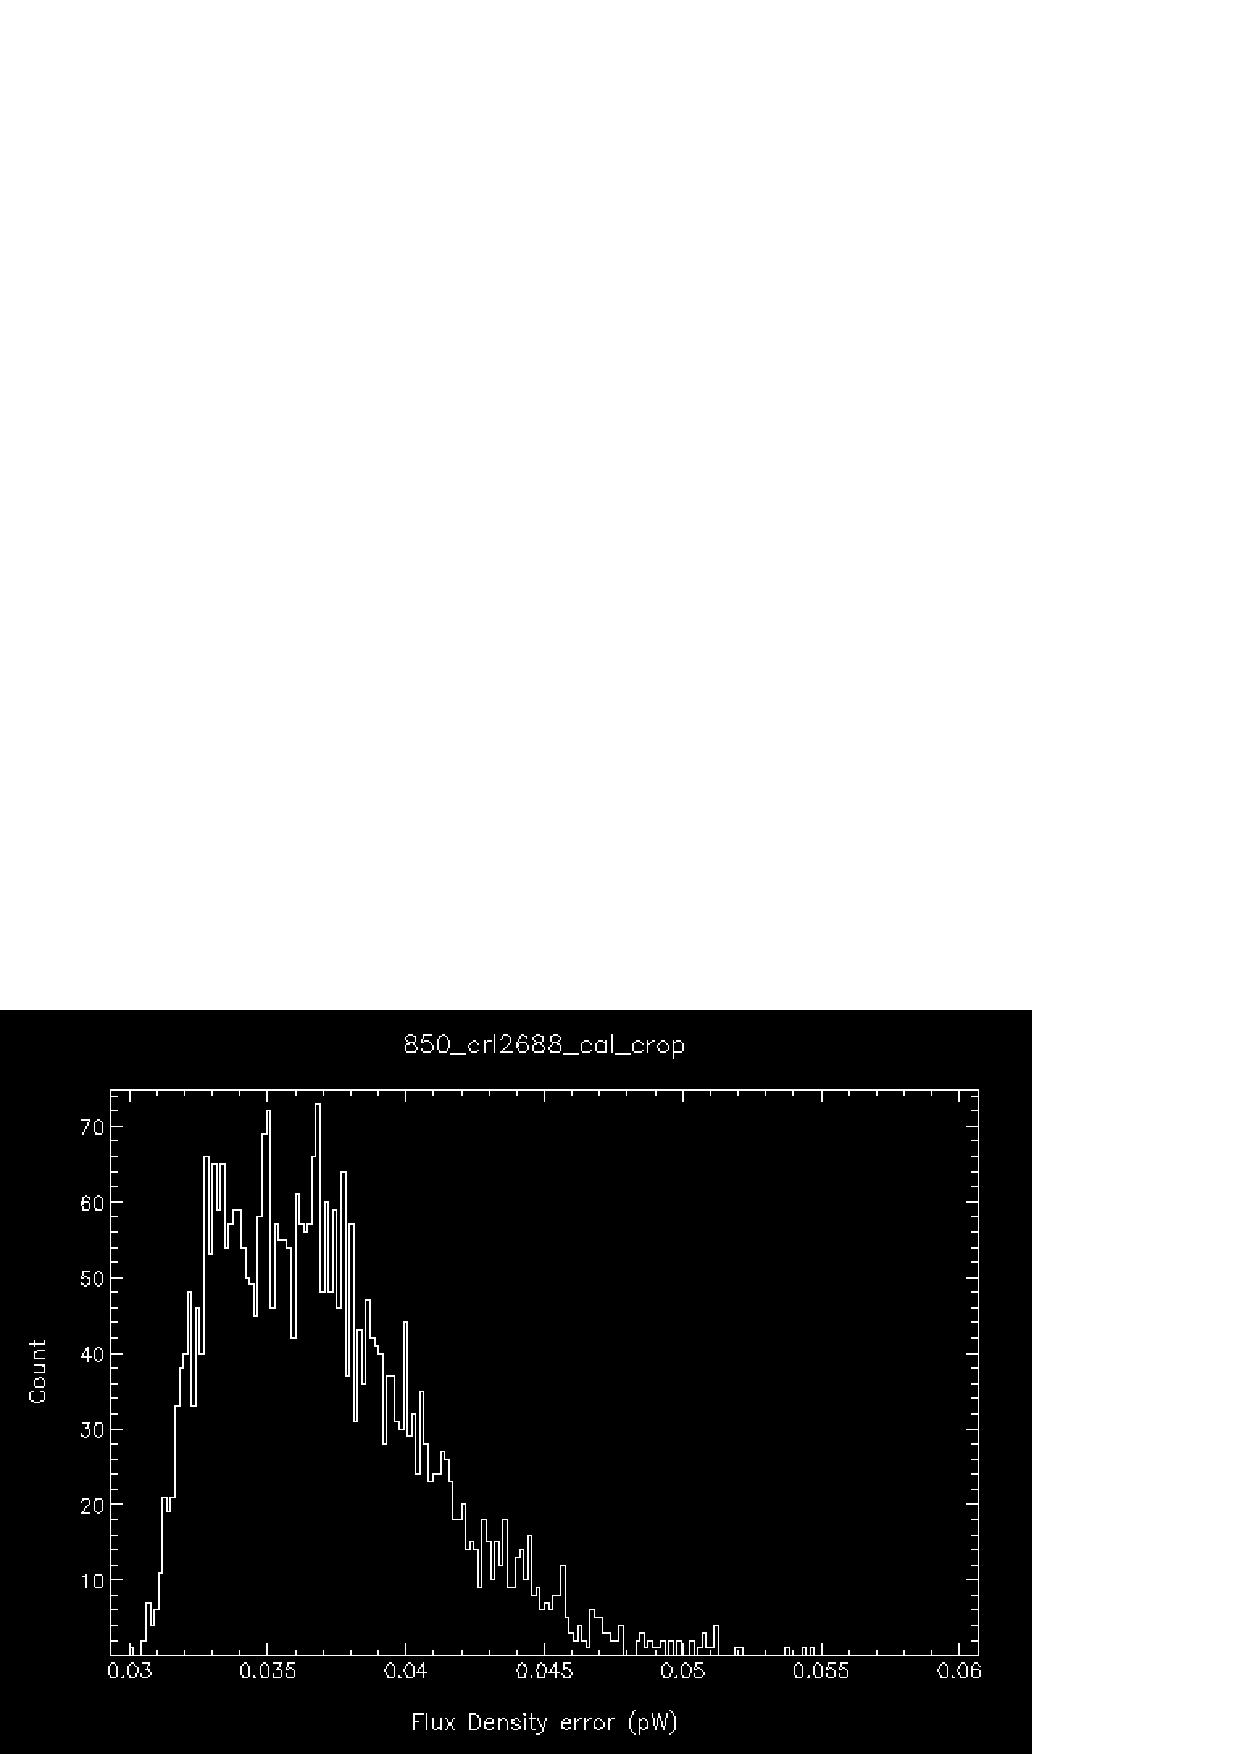
\includegraphics[height=6.5cm]{sc21_noihist}
\caption[The error map visualised in two ways.]{
  The error map viewed with \textsc{Kappa}:histogram.
}
\label{fig:noihisto}
\end{center}
\end{figure}

\subsubsection{Map statistics}

The \Kappa\ commands \histat\ and \stats\ are very similar and both
return a range of statistics describing any NDF. In addition to the
main data array they can be passed the error (\texttt{comp=err}), variance
(\texttt{comp=var}) and quality (\texttt{comp=qua}) arrays (if available).

The reported statistics include the pixel maximum and minimum,
standard deviation, number of pixels used and omitted, along with
pixel mode, mean and median.
\begin{myquote}
\begin{verbatim}
% stats comp=err map_cal_crop
\end{verbatim}
\end{myquote}

\textbf{Note:} the standard deviation of the data array will give a
similar result to the mean/median of the error array except with
additional contamination from sources.


\subsubsection{Viewing the noise histogram}

You can view a histogram of the error component with the
\textsc{Kappa} command \histogram. Again \param{comp=err} must be
specified.

\begin{myquote}
\begin{verbatim}
% histogram map_cal_crop comp=err numbin=200 style="color=white"
\end{verbatim}
\end{myquote}
The output is shown in the \cref{Figure}{fig:noihisto}{the figure
above}. For more information on the options for \histogram\ see
\kappasun.

\begin{figure}[b!]
\begin{center}
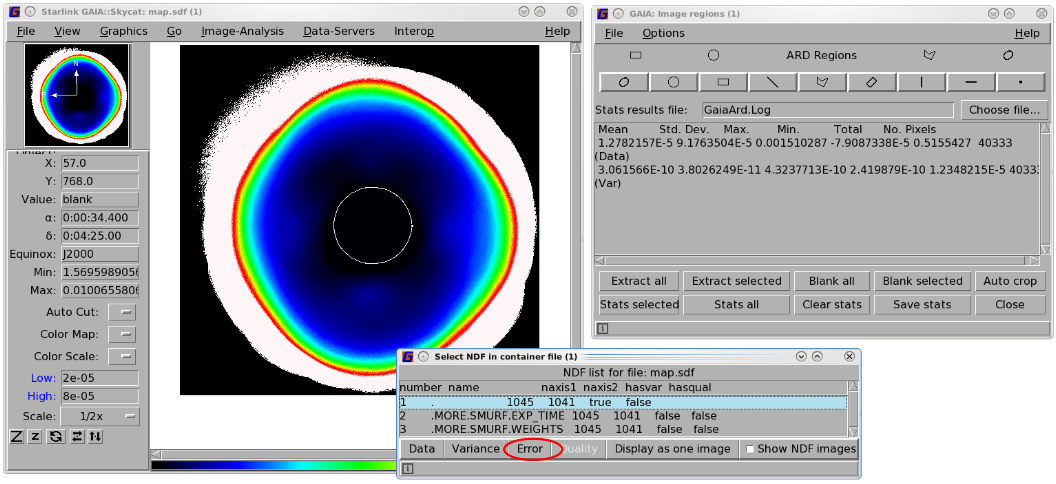
\includegraphics[width=\linewidth]{sc21_noigaia6}
\caption[The error map viewed with \gaia.]{
   The error component displayed with \gaia. After clicking the
   \texttt{Error} button you will have to rescale your map.
}
\label{fig:noigaia}
\end{center}
\end{figure}


\subsubsection{Examining the error map with GAIA}

It is also useful to view the error map itself. Open your reduced map
in \gaia, then select the \gaiathing{Error} button on the \gaiathing{Select NDF in
container file} window---see \cref{Figure}{fig:noigaia}{the figure
below}. You will need to adjust the scaling to view the error map properly.

To assess the noise in \gaia\ go to the toolbar on the main page and
click on \gaiathing{Image-Analysis$\Rightarrow$Image} regions. Next select
the region shape you would like to check and draw it on your map by clicking
and dragging the mouse. Then click the \gaiathing{Stats selected} button in the
\gaiathing{Image regions} window to get a report of the statistics.

\begin{latexonly}
\begin{center}
\begin{fmpage}{0.95\linewidth}
\vspace{0.1cm}

TIP: You can write out the error component of your map into a new file
using the \textsc{Kappa} command \ndfcopy. \newline
\texttt{         \% ndfcopy map comp=err map\_err}
\end{fmpage}
\end{center}
\end{latexonly}

\begin{htmlonly}
\textbf{TIP: You can write out the error component of your map into a new file
using the \textsc{Kappa} command \ndfcopy.  For example
\texttt{\% ndfcopy map comp=err map\_err}.}
\end{htmlonly}

\subsection{\xlabel{regridding}Regridding your Data}
\label{sec:regriddata}

To change the pixel size use the \Kappa\ command \compave. The following example
increases the pixel size from 4\,arcsec to 8\,arcsec by using a
compression factor of 2.

\begin{myquote}
\begin{verbatim}
% compave map map_regrid 2
\end{verbatim}
\end{myquote}

\begin{latexonly}
\begin{center}
\begin{fmpage}{0.95\linewidth}
\vspace{0.1cm}
TIP: Remember you can use \ndftrace\ if you are unsure of the pixel size.
\end{fmpage}
\end{center}
\end{latexonly}

\begin{htmlonly}
\textbf{TIP: Remember you can use \ndftrace\ if you are unsure of the pixel size.}
\end{htmlonly}

%they find that smaller pixels produce higher peak values (due to the smaller pixels producing less smoothing that larger pixels), and also converge faster (due to each pixel needing to be consistent with fewer bolometers). The average noise per pixel is higher for smaller pixels (as expected), and this means that the SNR level used for masking needs to be adjusted to get the same  mask produced using larger pixels.

\subsection{\xlabel{maskshow}Displaying masks}
\label{sec:maskshow}

Both \texttt{dimmconfig\_bright\_compact.lis} and
\texttt{dimmconfig\_bright\_extended.lis} configuration files use
masking. You can see where any masks were applied by viewing the Quality array in \gaia.

First open your map in \gaia. Select the top level NDF from list in
the pop-up window then click the \gaiathing{Quality} button. You will need to
rescale the map to bring out the masks--see \cref{Figure}{fig:qualdisp}{below}.

Each value in the QUALITY component of an NDF contains eight ``on/off''
flags used to indicate a specific binary property of the pixel. The
first three of these flags indicate whether a pixel is inside or outside a
specific mask (1=\texttt{AST}, 2=\texttt{FLT} or 3=\texttt{COM}).

There are four potential values for the common combination of
\texttt{AST} and \texttt{FLT} masks:
\\*\\*
0 = pixel is inside both \texttt{FLT} and \texttt{AST} mask (i.e. is a source pixel)\\
1 = pixel is inside \texttt{AST} mask but not \texttt{FLT} mask\\
2 = pixel is inside \texttt{FLT} mask but not \texttt{AST} mask\\
3 = pixel is inside neither mask (i.e. is a background pixel)
\\*\\*
The maximum quality value increases from 3 to 7 if \texttt{COM} masking is included.

You can see which bit is used for each mask with \showqual.
\begin{myquote}
\begin{verbatim}
% showqual map count
\end{verbatim}
\end{myquote}

As an example, you can set bad all pixel outside the \texttt{FLT} mask by doing:

\begin{myquote}
\begin{verbatim}
% setbb map 2
\end{verbatim}
\end{myquote}
\vspace{0.3cm}

\textbf{Contouring a mask over your map}\\*
If you would like to plot a mask over your map you will need to copy
out the QUALITY component of the data to a separate file using \texttt{ndfcopy}.
\begin{myquote}
\begin{verbatim}
% ndfcopy comp=qua map map_mask
\end{verbatim}
\end{myquote}
Then open your map in \gaia\ and contour the mask NDF on top. See
\cref{Figure}{fig:maskdisp}{the figure below}.

For more information on the use of masks by \makemap\ and the
parameters that affect them see \cref{Section}{sec:tweak}{Tailoring
your Reduction}.

\myfig{sc21_qualitygaia}{[t!]}{width=0.9\hsize}{fig:qualdisp}{}{
   Using \gaia\ to display the mask applied by the map-maker. Select the
   QUALITY components of your map.
}

\myfig{sc21_dispmask3}{[b!]}{width=0.95\hsize}{fig:maskdisp}{}{
   Using \gaia\ to display your map with the \texttt{AST} mask used by
   the map-maker contoured on top.
}


\subsection{\xlabel{match_filter}Point-source extraction: the matched filter}
\label{sec:mf}

This effectively fits a single Gaussian point spread function (PSF), centered over
every pixel in the map, and applies a background suppression filter to
remove any residual large-scale noise.

Cosmology maps usually contain very faint sources that often need
extra help extracting. The \picard\ recipe
\xref{\drrecipe{SCUBA2\_MATCHED\_FILTER}}{sun265}{SCUBA2_MATCHED_FILTER}
can be used to improve point-source detectability.

The matched filter works by smoothing the map and PSF with a broad
Gaussian and then subtracting from the originals. The images are then
convolved with the modified PSF. The output map should be used
primarily for source detection only. Although the output is normalised
to preserve peak flux density, the accuracy of this depends on how
closely the real PSF matches the telescope beam size. In the case of
nearby sources, each ends up contributing flux to both peaks.

\begin{myquote}
\begin{verbatim}
% picard -recpars mypar.lis SCUBA2_MATCHED_FILTER 850_map_cal_crop.sdf
\end{verbatim}
\end{myquote}

As in the example parameter file below we have requested the
background should be estimated by first smoothing the map and PSF with
a 15-arcsec Gaussian.
\begin{myquote}
\begin{verbatim}
[SCUBA2_MATCHED_FILTER]
SMOOTH_FWHM = 15
\end{verbatim}
\end{myquote}
\vspace{0.4cm}

This is a fairly common technique used throughout the extra-galactic
sub-millimetre community to identify potential sources. A full
description of the matched filter principle is given in
\cref{Appendix}{app:mf}{SCUBA-2 Matched Filter}, while the \textsc{Picard}
manual gives full details of all the available parameters.

\subsection{\xlabel{clumps}Clump finding}
\label{sec:clumps}
\label{sec:clumpfind}
The \cupid\ application \findclumps\ can be used to generate a clump
catalogue. It identifies clumps of emission in 1, 2 or 3D NDFs. The
user can select from the clump finding algorithms FellWalker,
Gaussclumps, ClumpFind or Reinhold and must supply a configuration
file specific to each method. See the \xref{\textsc{Cupid}
manual}{sun255}{} for descriptions of the various algorithms.

The result is returned as a catalogue in a text file and as a NDF
pixel mask showing the clump boundaries.

\begin{myquote}
\begin{verbatim}
% findclumps in=S2map.sdf out=clumpmap.sdf outcat=clumps.FIT logfile=clumps.log \
  config=^config.dat method=fellwalker rms=25 shape=polygon
\end{verbatim}
\end{myquote}

The shape option allows \findclumps\ to create an STC-S description
(polygonal or elliptical) for each clump. These are added as extra
columns to the output catalogue.
\\*\\*
\begin{minipage}[t]{0.12\linewidth}
\textbf{Polygon}
\end{minipage}
\begin{minipage}[t]{0.85\linewidth}
Each polygon will have, at most, 15 vertices. For two-dimensional data
the polygon is a fit to the clump's outer boundary (the region
containing all good data values). For three-dimensional data the
spatial footprint of each clump is determined by rejecting the least
significant 10\% of spatial pixels, where "significance" is measured
by the number of spectral channels that contribute to the spatial
pixel. The polygon is then a fit to the outer boundary of the
remaining spatial pixels.

\end{minipage}

\begin{minipage}[t]{0.12\linewidth}
\textbf{Ellipse}
\end{minipage}
\begin{minipage}[t]{0.85\linewidth}
All data values in the clump are projected onto the spatial plane and
"size" of the collapsed clump at four different position angles---all
separated by 45$^\circ$---is found. The ellipse that generates the
same sizes at the four position angles is then found and used as the
clump shape.
\end{minipage}

\myfig{sc21_plotstcshapes}{[h!]}{width=0.99\linewidth}{fig:stcshapes}{
  Overlaying a clump catalogue in \gaia.}{
  STC shapes displayed over the input map with \gaia. To overlay your clumps
  in this way open you map with \gaia. Under the \gaiathing{Image-Analysis}
  menu select \gaiathing{Positions...} followed by \gaiathing{Import CUPID
  catalogue...} In the pop-up window select the \texttt{.FIT} file
  generated by \findclumps\ and ensure the \gaiathing{STC shape} box is
  checked before importing.
}


\subsection{\xlabel{provenance}Map provenance \& configuration parameters}
\label{sec:prov}

You may want to check a reduced file to determine which raw files went
into it and what configuration parameters were used with the
map-maker. There are a number of useful \Kappa\ commands to help you
with this:

\textbf{Map provenance}\\
\provshow\ will list all the NDFs that were used in the creation of
your map, while \hislist\ will show a truncated list of input files
but will list every configuration parameter used by the map-maker.
This includes all the hidden default values as well as those specified
in your supplied configuration file. These commands are executed like
this:
\begin{myquote}
\begin{verbatim}
% provshow 850map.sdf
% hislist 850map.sdf
\end{verbatim}
\end{myquote}

\textbf{Map-maker parameters}\\
The task \configmeld\ will identify what configuration parameters were
used by the map-maker when your data were reduced. \configmeld\
requires a visual-differences tool to be installed on your machine;
those currently recognised are

\htmladdnormallink{\texttt{meld}}{http://meldmerge.org/}\latex{\footnote{\texttt{http://meldmerge.org/}}},
\htmladdnormallink{\texttt{opendiff}}{http://developer.apple.com/},
\htmladdnormallink{\texttt{diffmerge}}{http://www.sourcegear.com/diffmerge},
\htmladdnormallink{\texttt{kdiff3}}{http://kdiff3.sourceforge.net},
\htmladdnormallink{\texttt{tkdiff}}{http://sourceforge.net/projects/tkdiff}, and
\htmladdnormallink{\texttt{diffuse}}{http://diffuse.sourceforge.net},
and are searched for in that order. It will compare the
configuration parameters for two reduced maps or configuration files
(which can be mixed and matched). The follow example illustrates two
ways to run it.

\begin{myquote}
\begin{verbatim}
% configmeld 850map1.sdf 850map2.sdf
% configmeld 850map1.sdf ^mydimmconfig2.lis
\end{verbatim}
\end{myquote}
Another useful command is the \Kappa\ command \configecho.
This is very versatile and will display the name and value of one or
all configuration parameters either from a configuration file or from
the history of an NDF.

The first example below will return the value of \texttt{numiter} from
the map \texttt{850map.sdf}. The second example will display the values of all
the parameters in \texttt{850map.sdf} and will prefix them with a `+' if they
differ from the the values given in \texttt{dimmconfig.lis}.

\begin{myquote}
\begin{verbatim}
% configecho name=numiter config=! ndf=850map.sdf
% configecho name=! config=^dimmconfig.lis ndf=850map.sdf
\end{verbatim}
\end{myquote}

\clearpage
\section{\xlabel{tweak}Tailoring your Reduction}
\label{sec:tweak}


\subsection{ Adding and amending parameters}
The default configuration file \texttt{dimmconfig.lis} contains all of
the parameters the most users would wish to play with.

\textbf{You can create your own personalised configuration file from
scratch or copy one of the provided ones to your local directory and
edit it.}

The first line of each specialised configuration file is always a path
to the recipe from which it is derived. These paths all lead to
recipes in the \starlink\ tree which cannot be edited. If you are
creating your own file from scratch, make sure to include this
reference to an existing configuration file on the first line.
Remember any parameters appearing your configuration file
automatically override their values in the default file (see
\cref{Figure}{fig:configtree}{this figure}.

You can also add or amend parameters by listing them directly on the
command line. They are appended to the configuration filename as a
comma separated list as shown in the example below. Be sure to include
all the necessary quotation marks.

\begin{myquote}
\begin{verbatim}
% makemap in='s8*.sdf' out=850map method=iterate \
config='"^dimmconfig.lis,numiter=20,exportndf=(flt,noi),itermap=1"'
\end{verbatim}
\end{myquote}

\textbf{What parameters can be changed?}\\*

Any of the parameters listed in \texttt{dimmconfig.lis} can be
changed. For comprehensive list of the parameters in
\texttt{dimmconfig.lis} see \cref{Appendix}{app:dimm}{an appendix}.

The map-maker uses other parameters beyond those described in the
configuration files. These can be found in the default makemap file,
smurf\_makemap.def. This file lives in your \$SMURF\_DIR directory or
online at the \starlink\ \htmladdnormallink{github
repository}{https://github.com/Starlink/starlink/blob/master/applications/smurf/defaults/smurf\_makemap.def}
\latex{\footnote{\texttt{https://github.com/Starlink/starlink/blob/master/applications/smurf/defaults/smurf\_makemap.def}}}.
We do not advise users to alter any of these default parameters
however.

\begin{latexonly}
\begin{center}
\begin{fmpage}{0.95\linewidth}
\vspace{0.1cm}
TIP: If you wish to disable an active parameter in the default file,
set it as \texttt{<undef>} in your personalised file.
\end{fmpage}
\end{center}
\end{latexonly}

\begin{htmlonly}
\textbf{TIP: If you wish to disable an active parameter in the default
file, set it as \texttt{<undef>} in your personalised file.}
\end{htmlonly}


\textbf{Note:} any parameter can be made wavelength dependent by
adding the prefix \texttt{450.} or \texttt{850.}, e.g.
\texttt{flt\_edge\_largescale} applies to both 450\,$\mu$m and
850\,$\mu$m whilst \texttt{450.flt\_edge\_largescale} applies to
450\,$\mu$m only. Be aware that if both are specified, unqualified
values (no prefix) take priority over qualified values.

\subsection{\xlabel{inter}Writing out models \& intermediate maps}


\subsubsection{itermap}
Setting the parameter \texttt{itermap~=~1} writes out an astronomical map after each
iteration. Setting \texttt{itermap~=~2} adds the QUALITY component.
These can be visually inspected with

\begin{myquote}
\begin{verbatim}
% gaia 850map.more.smurf.itermaps
\end{verbatim}
\end{myquote}
to help determine an appropriate number of iterations. This is useful
when a fixed number of iterations have been requested (i.e. a positive
value for \texttt{numiter}) and the map solution diverges before
they have completed.

\textbf{shortmaps}\\
If the parameter \texttt{shortmaps} is non-zero, a map is made from
every group of adjacent timeslices (specified by the parameter).
These are stored as an NDF extension and can be viewed \gaia.

\begin{latexonly}
\begin{figure}[ht!]
\begin{center}
\begin{fmpage}{0.95\linewidth}
\vspace{0.2cm}
\hspace{2mm}
\textbf{Viewing ITERMAPs}

\vspace{0.5cm}

\begin{minipage}[c]{0.65\linewidth}

\begin{myquote}
\begin{verbatim}
% stackframes map.more.smurf.itermaps \
sort=false map_itermaps
\end{verbatim}
\end{myquote}
\end{minipage}
\hspace{0.3cm}
\begin{minipage}[c]{0.29\linewidth}
Stack the individual itermaps into a single cube.
\end{minipage}

\vspace{0.5cm}

\begin{minipage}[c]{0.65\linewidth}
\centering
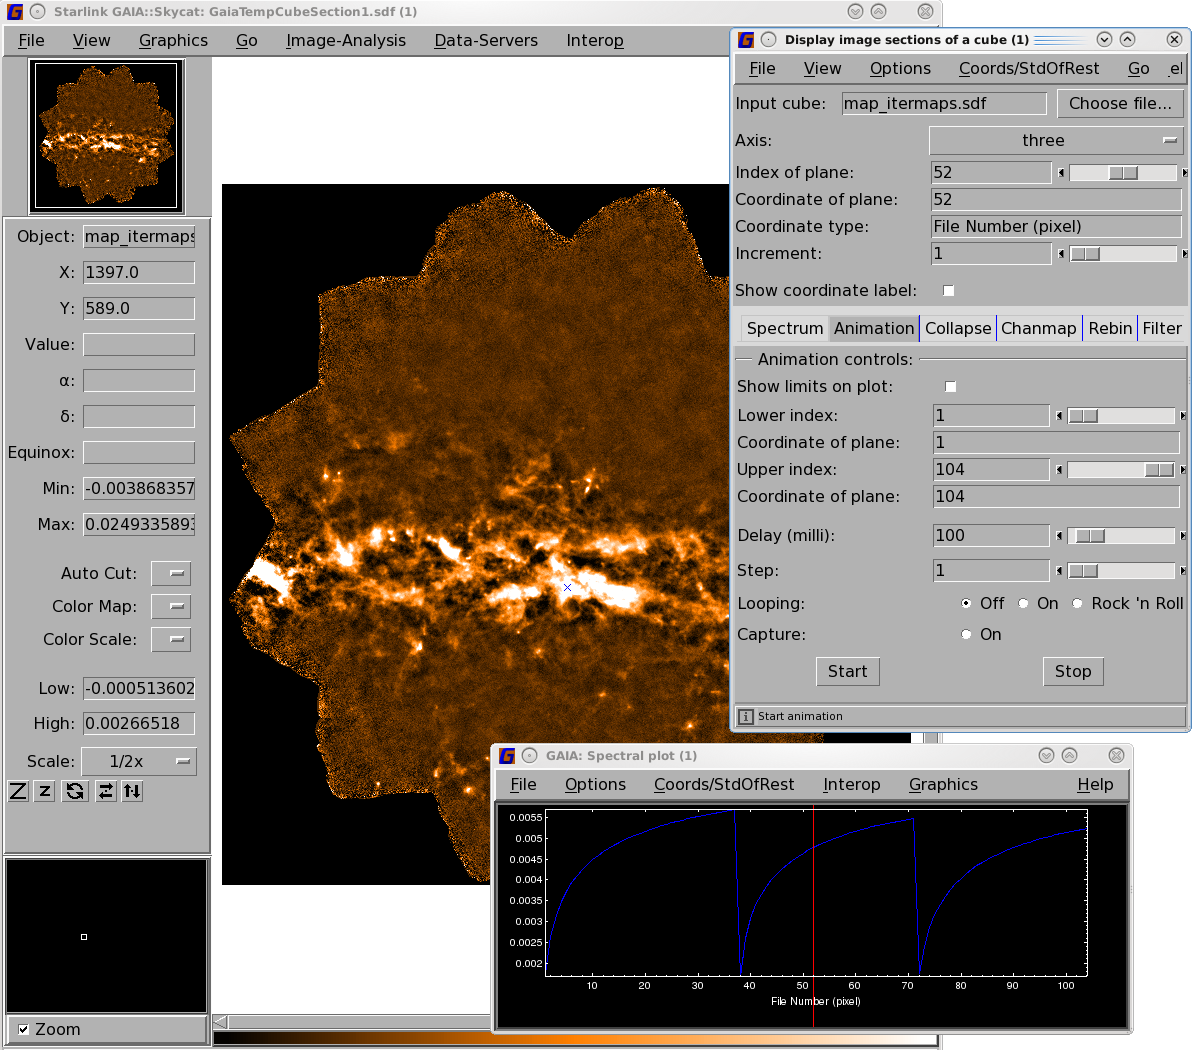
\includegraphics[width=0.95\textwidth]{sc21_itermaps_anim}

\end{minipage}
\hspace{0.3cm}
\begin{minipage}[c]{0.29\linewidth}
The output map map\_itermaps can be opened with \gaia. The data used
in this example is the Galactic map reduced in
\cref{Section}{sec:bright_ex}{dimmconfig\_bright\_extended.lis}. The
Spectral plot window shows the value for a single pixel and the three
chunks are easily identified. You can select the \gaiathing{Animation} tab
in the \gaiathing{Display image sections} window and click
\gaiathing{Start} to loop through the itermaps for each iteration.  The
`movie' will appear in the main \gaia\ window.
\end{minipage}

\vspace{0.7cm}

\begin{minipage}[c]{0.65\linewidth}
\centering
\hspace{0.5mm}
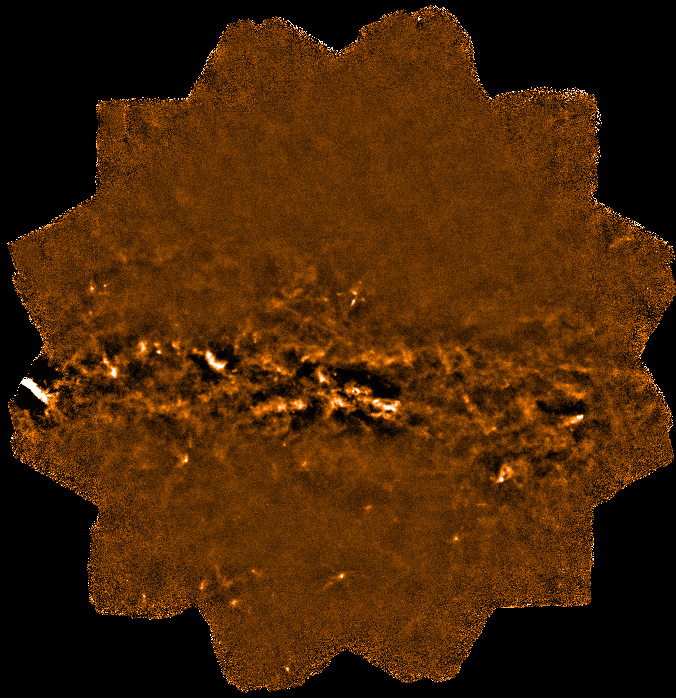
\includegraphics[width=3cm, height=3cm]{sc21_iter1}
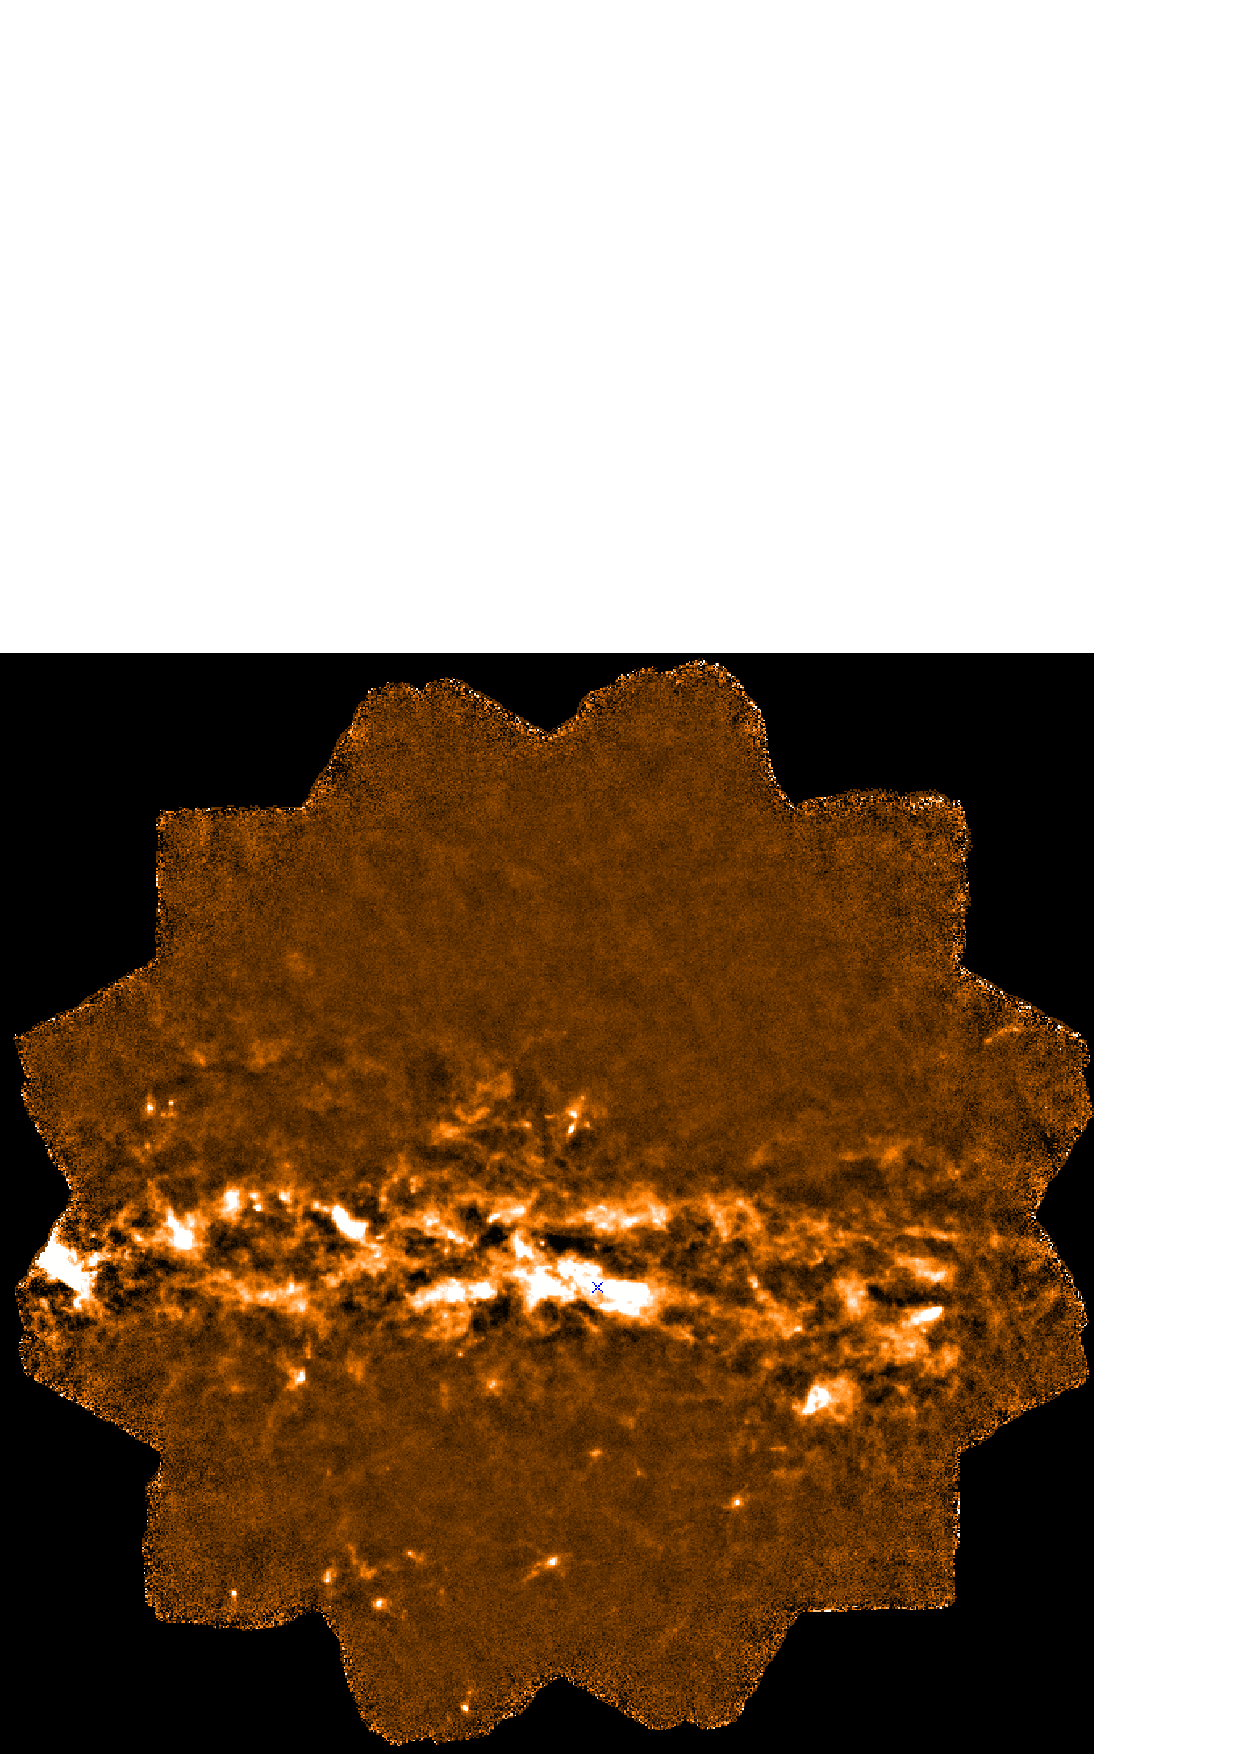
\includegraphics[width=3cm, height=3cm]{sc21_iter2}
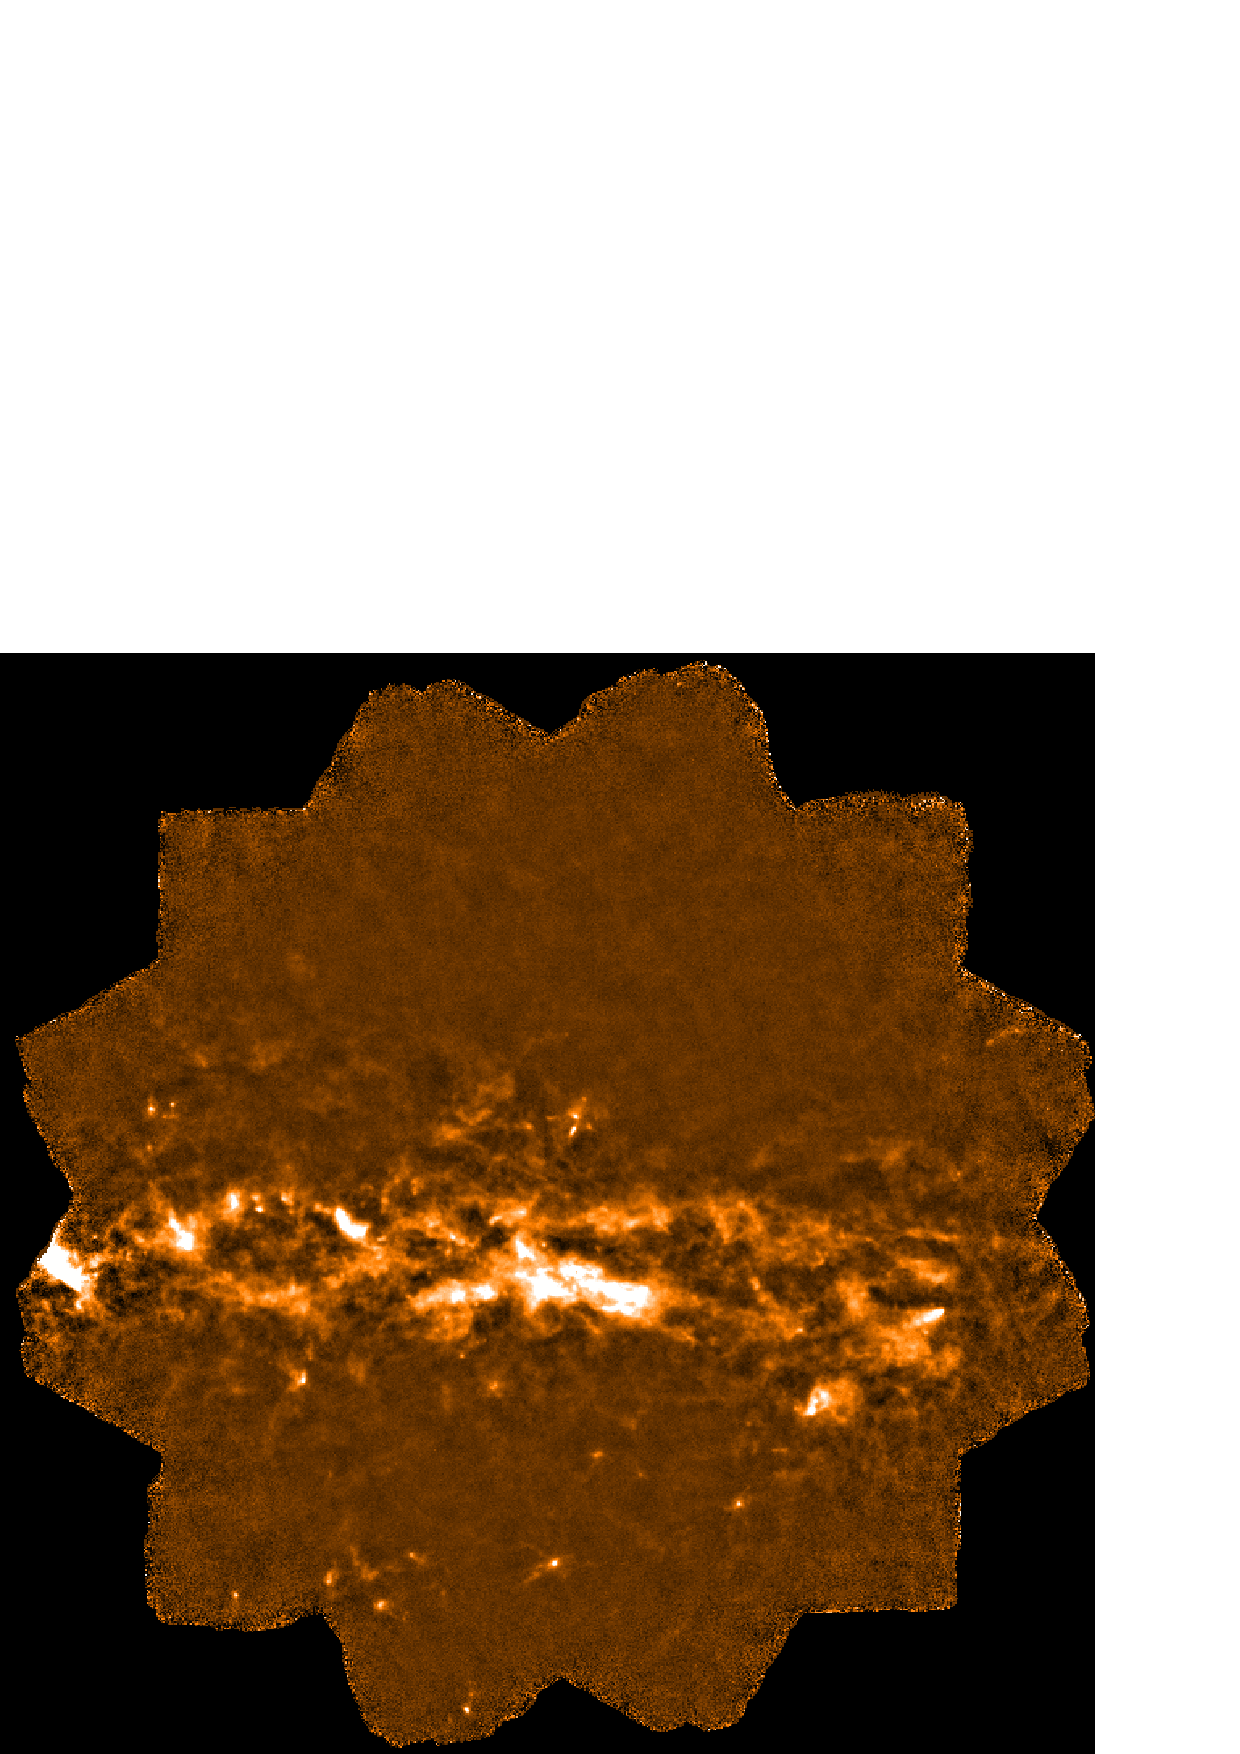
\includegraphics[width=3cm, height=3cm]{sc21_iter31}
\vspace{0.2cm}
\end{minipage}
\hspace{0.3cm}
\begin{minipage}[c]{0.29\linewidth}
These windows show the itermaps map at 1, 10, and 30 iterations. A
specific iteration can be selected using the `Index of plane' slider
on the `Display image sections' window.
\vspace{0.2cm}
\end{minipage}
\end{fmpage}
\end{center}
\caption[View maps for each iteration]{
  \small Example using the \smurf\ command \stackframes\ and
  \gaia\ to view the `itermaps' map for each iteration.
}
\label{fig:stack}
\end{figure}
\end{latexonly}

% The minipages used for the dvi version give latex2html problems.
\begin{htmlonly}
\label{fig:stack} \htmladdimg{sc21_view_itermaps.png}
Figure: Example using the \textsc{Smurf} command \task{stackframes} and
\gaia\ to view the `itermaps' map for each iteration.
\end{htmlonly}

\begin{myquote}
\begin{verbatim}
% gaia 850map.more.smurf.shortmaps
\end{verbatim}
\end{myquote}

\textbf{Note:} You can view the shortmaps and itermaps more
conveniently by stacking them into a single cube using the \smurf\
command \stackframes. This cube can then be viewed as a
`movie' with \gaia, using the animation option to loop through the
itermaps. See \cref{Figure}{fig:stack}{the box above} for instructions.

\subsection{exportmodel}

This parameter has been discussed in
\cref{Section}{sec:export}{Exporting individual models} and allowed
you to see the model that was fit for each component specified by the
\texttt{modelorder} parameter.

\subsection{\xlabel{filt}Adjusting the filtering}
\label{sec:filt}

Some of the most important parameters to experiment with are the
filtering options. By default the low-pass filter is applied once
during the pre-processing stage and is turned off for the iterative
steps. The high-pass filter is only specified during the iterative
steps and its selected value is crucial for maps containing extended
emission. All the parameters dealing with the \texttt{FLT} model can
be found in \cref{Appendix}{app:par_full}{Configuration Parameters: dimmconfig.lis}.

The maximum spatial scale of structure that can be recovered by the
map-maker is determined by the scanning speed and frequency cut
applied to the data:

\begin{equation}
\frac{\mbox{speed}\;(''/\mbox{s)}}{\mbox{frequency cut}\;(\mbox{Hz)}}=\mbox{scale size}\;('')
\end{equation}

The filtering options set in \texttt{dimmconfig.lis} are:

\texttt{450.flt.filt\_edge\_largescale~=~600} \\
\texttt{850.flt.filt\_edge\_largescale~=~300}.

To make your life easier, these parameters allow you to specify the
filter limits in terms of spatial scale in arcsecs---in this case
300\,arcsec at 850\,$\mu$m and 600\,arcsec at 450\,$\mu$m. For example
at 850\,$\mu$m, recovering scales of 300\,arcsec at a scan speed of
600\,arcsec/sec (default for a 1 degree \textsc{pong}) corresponds to
a frequency 2\,Hz.

Choosing a high-pass filter is especially important for the recovery
of extended emission. The \texttt{dimmconfig\_bright\_extended.lis}
recipe sets \texttt{flt.filt\_edge\_largescale~=~480} (i.e. both 450
and 850\,$\mu$m). Be aware that increasing filtering scales decreases
the flatness of your background. A compromise must be made between
extended structure and the flatness of your map. See
\cref{Figure}{fig:fltcompare}{the figure below} for an illustration of
the effect of \texttt{flt.filt\_edge\_largescale} on your map.

The scanning speeds are fixed for a given observing mode; you can find
out the speed at which your data were taken from the
\texttt{SCAN\_VEL} parameter in the FITS header (see
\cref{Section}{sec:fitsheader}{Headers and file structure}).


\myfigduo{sc21_brex_19}{sc21_brex_18}{}{width=0.46\linewidth}{fig:fltcompare}{7mm}{
  Illustrating the effects of high-pass filtering}{
  Highlighting the effects of high-pass filtering on your map.
  \textbf{(Left)} Map made with \texttt{850.flt.filt\_edge\_largescale~=~300}.
  \textbf{(Right)} Map made with \texttt{850.flt.filt\_edge\_largescale~=~1000}.
  All other configuration parameters remain the same.
}

\subsection{\xlabel{fitcom}Fitting COM for each sub-array}
\label{sec:fitcom}

A useful option to improve the flatness of your maps is to fit the
\texttt{COM} model independently for each sub-array. This is
particularly effective if you find you have one sub-array noisier than
the others.

This comes with the warning however that you will lose information on
any scales larger than the area covered by a single sub-array. It is
therefore not recommended if you have very large-scale extended
structure.

To initialise this option set \texttt{com.perarray~=~1}.


\subsection{\xlabel{noibox}Flagging bad data}
\label{sec:noibox}

It is possible to down-weight data that have higher noise by setting
the parameter \texttt{noi.box\_size}. If this is set (i.e. non-zero)
then the length of time over which the noise is determined can be
specified in time samples (positive values) or seconds (negative
values). By default this is set to zero and the whole time stream is
used giving a single variance for each bolometer. This variance is
used to weight the data for subsequent iterations, hence more finely
estimated noise levels are preferable.

The parameter \texttt{noi.box\_size} helps remove `scuffs' or other
noise artifacts you might see in your error map due to a sub-array (or
arrays) temporarily jumping to a higher noise state. The default file
has \texttt{noi.box\_size~=~$-$15} (i.e. half a sub-scan). As the
value tends to $-$1 (one second) we find some of the source signal being
down-weighted. Higher than this $-$15 value and the map-maker becomes
less sensitive to the higher noise states.

Other parameters you may want to utilise include \texttt{flagfast} and
\texttt{flagslow}. You may find that setting \texttt{flagfast} to less
than the default of 1000\,arcsec/sec will help reduce the effect of any
`smearing' of sources (and of noise) in maps, while setting
\texttt{flagslow} greater than the default of 300\,arcsec/sec helps to
flatten the edges of maps. To determine reasonable values for your
 dataset you should do \jcmtstate\ and view the scan speed using
\topcat---see \cref{Section}{sec:scan}{Displaying scan patterns} for
details.

\subsection{\xlabel{mask}Masking options}
\label{sec:mask}

ast.skip doesn't subtract the ast model for the first X iterations.
The map can then do FLT masking on. It starts from scratch with each
iteration and gets a good map from FLT masking.


The \texttt{AST}, \texttt{FLT} and \texttt{COM} models each have a
number of common masking options. The main ones are
\texttt{xxx.zero\_circle}, \texttt{xxx.zero\_lowhits},
\texttt{xxx.zero\_snr} and \texttt{xxx.zero\_snrlo}. Masking comes
with different restrictions and sensitivities depending on the model
in question.

\texttt{AST} masking is the option we recommend. On each iteration the
map is constrained to zero at all points outside the masked region and
the \texttt{AST} model is estimated based only on data inside the
mask.

\texttt{FLT} masking is used to omit bright sources from the estimate
of the low frequency background subtracted from the residuals on each
iteration. This can help prevent ringing in the final map. S/N based
\texttt{FLT} masking cannot be used on the first iteration and
\texttt{FLT} masking should be used sparingly to aid convergence (it
is limited to the first two iterations by default by
\texttt{flt.zero\_niter~=~2}).

\texttt{COM} masking is used to omit very bright sources from the
estimate of the common-mode signal, this can prevent sources being
rejected due to their dissimilarity to the common-mode. S/N based
\texttt{COM} masking cannot be used on the first iteration and the
mask should always be small.

For the rest of this section we will concentrate on \texttt{AST}
masking only. \texttt{ast.zero\_circle} defines a circle is defined to
mask out the source, with everything outside this circle being
constrained to zero. This is utilised in
\texttt{dimmconfig\_bright\_compact.lis} by the \texttt{AST} model as
the source is expected to be very compact with a flat background. The
default size of this circle is 60\,arcsec, but this can adjusted by
altering \texttt{ast.zero\_circle}. The position of this circle
defaults to the centre of the map. You can specify alternative
coordinates if this is not appropriate.

\texttt{ast.zero\_lowhits} allows masking based on the number of data
samples in a pixel. For the \texttt{AST} model this means that
spurious regions of emission at the edges of the map where exposure
time is low are not included in the source mask. See the documentation
in \cref{Appendix}{app:par_full}{Configuration Parameters:
dimmconfig.lis} for more information on each.

Finally there is signal-to-noise based masking as utilised by
\texttt{dimmconfig\_bright\_extended.lis}. It uses the parameter
\texttt{ast.zero\_snr} to define a mask based on the S/N. The default
is 5, meaning that pixels below an S/N of 5\,$\sigma$ will be set to
zero. This is dynamic with the S/N mask being re-determined after each
iteration. Setting \texttt{ast.zero\_snr} too low can cause noise
spikes to be interpreted as signal. Instead, \texttt{ast.zero\_snrlo}
can be set which allows the mask to grow to include pixels with an S/N
down to \texttt{ast.zero\_snrlo}. This typically improves the
resulting map so is well worth experimenting with.

An alternative to setting \texttt{ast.zero\_snrlo} is to smooth the
S/N mask by setting the parameter \texttt{ast.zero\_snr\_fwhm}.

Remember for all \texttt{AST} masking to include
\texttt{ast.zero\_notlast~=~1} so that mask is not applied on the
final iteration. This means that the background regions in the map are
only generated by this single, final iteration.

An alternative to S/N masking is to supply an external mask using the
\texttt{REF} parameter. Setting the parameter
\texttt{ast.zero\_snr\_fwhm} allows you to automate this step for a
specific case. Here, the map-maker is run once, then the mask
generated by \texttt{ast.zero\_snr} is smoothed by a Gaussian (of
`FWHM' arcsecs) and the map-maker is re-run with this smoothed mask
supplied as an external mask. You can supply your own external mask
however by following the instructions in the next section.

Multiple masks are combined according to the \texttt{ast.zero\_union}
parameter (there are also corresponding \texttt{FLT} and \texttt{COM}
ones). If this parameter is true (i.e. non-zero) then the two masks
will be combined to act as one large mask (the union of the individual
masks). Hence a pixel will be flagged/masked if it falls within either
mask (rather than being required to fall in both). The alternative is
a false (i.e. zero) value; this means that only pixels that fall into
both masks independently will be flagged/masked. Here, only the
intersection of the masks is considered the final masked area.

For example, if you find an S/N mask allow bright regions to develop
towards the edges of your map, you can force these to zero by using
the intersection of the S/N mask with a `low-hits' mask.

There are a number of options
available which build on the default recipe. The simplest is to set
the configuration parameter \texttt{ast.zero\_snrlo} which allows the
mask to grow organically as the \texttt{AST} model evolves.


\subsection{\xlabel{maskbe}Supplying an external mask}
\label{sec:maskbe}

As an S/N mask is redetermined after each iteration it varies as the
map varies which can sometimes cause convergence problems. The mask
will also depend on the amount of data going into the map and the
pixel size. An externally supplied mask is fixed and tells the
map-maker where you expect the emission to be.

The sequence below is a summary of the procedure for generating and
supplying an external mask. In this example the mask is generated from
the map produced by an initial run through the map-maker.
Alternatively maps from other telescopes can be used.

These steps are followed in the example in
\cref{Section}{sec:bright_ex}{Extended galactic sources}.

\textbf{(1)} Generate a map covering your region. This may be by simply
running the map-maker on your data as shown below.
\begin{myquote}
\begin{verbatim}
% makemap in='s8*.sdf' out=850map method=iterate \
config='"^dimmconfig_bright_extended.lis"'
\end{verbatim}
\end{myquote}
The alternative is to access a map from a different dataset or even a
different telescope, e.g. a map downloaded from the Herschel Science
Archive. For instructions on converting from fits format to NDF see
\cref{Appendix}{app:convert}{Converting a Herschel map to NDF}.
\\*\\*
\textbf{(2)} Make a signal-to-noise map using the \Kappa\ command \makesnr.
\begin{myquote}
\begin{verbatim}
% makesnr 850map 850map_snr
\end{verbatim}
\end{myquote}
\textbf{(3)} This S/N map is thresholded to set everything below 3$\sigma$ to 0 and
everything above to 1.
\begin{myquote}
\begin{verbatim}
% thresh 850map_snr 850map_mask thrlo=3 newlo=0 thrhi=3 newhi=1
\end{verbatim}
\end{myquote}
In the step above you can set everything below 3$\sigma$ to
\texttt{bad} and use this as your mask. However this generates a hard
3$\sigma$ cut-off to your map which is unrealistic for the real data.
Instead the following 2 steps are performed to smooth the edges of the
mask.
\\*\\*
\textbf{(4)} The thresholded map is smoothed with a Gaussian filter
of FWHM of 5 pixels (=\,20\,arcsec). Then it is again thresholded, this time
keeping everything above 5\,\% of the 0 level as the mask and setting
the rest to \texttt{bad}.
\begin{myquote}
\begin{verbatim}
% gausmooth 850map_mask 850map_mask_sm fwhm=5
% thresh 850map_mask_sm 850map_mask_zm thrlo=0.05 newlo=bad thrhi=0.05 newhi=1
\end{verbatim}
\end{myquote}
Finally the map is re-made with this mask supplied as an external
file. Notice that the extra parameters required to pick up this external
mask are being appended to the configuration file on the command line
rather than editing the file itself.
\begin{myquote}
\begin{verbatim}
% makemap in='s8*.sdf' out=850map_zm method=iterate \
config='"^dimmconfig_bright_extended.lis,ast.zero_mask=1,ast.zero_snr=0"' \
ref=850map_mask_zm
\end{verbatim}
\end{myquote}

\subsection{\xlabel{skyloop}Skyloop}
\label{sec:skyloop}

Traditionally, the map-maker divides a non-contiguous sequence of time
series data into chunks. It processes each chuck independently
before co-adding them as a final step in the the reduction---see
\cref{Figure}{fig:skyloop}{figure below}.

This means for each chunk the map-maker has to start from scratch
determining the \texttt{AST} model and the benefit of long integration
times spent building up the signal is lost. Recipes which use
signal-to-noise masks especially suffer from this approach as the
signal-to-noise in each individual chunk can remain low and fainter
extended structure is not recovered.

This new \skyloop\ command runs \makemap\ multiple times
performing just a single iteration on each occasion. It starts by
performing a single iteration of \makemap\ from which a final
co-added map is generated. This map is then supplied as an initial
estimate of the sky for the next loop through \makemap. On
this next iteration, the initial sky estimate is subtracted from the
cleaned time-series data and the \texttt{COM}, \texttt{GAI},
\texttt{FLT}, \texttt{EXT} models are subtracted. This produces a new
model of the sky (from the current iteration) to which the sky
estimate (from the previous iteration) is then added. In this way the
signal from all of the chunks is built up over the iterations and is
all included in the final map estimate when convergence is reached.
See \cref{Figure}{fig:skyloop}{the diagram below}.

\begin{figure}[h!]
\centering
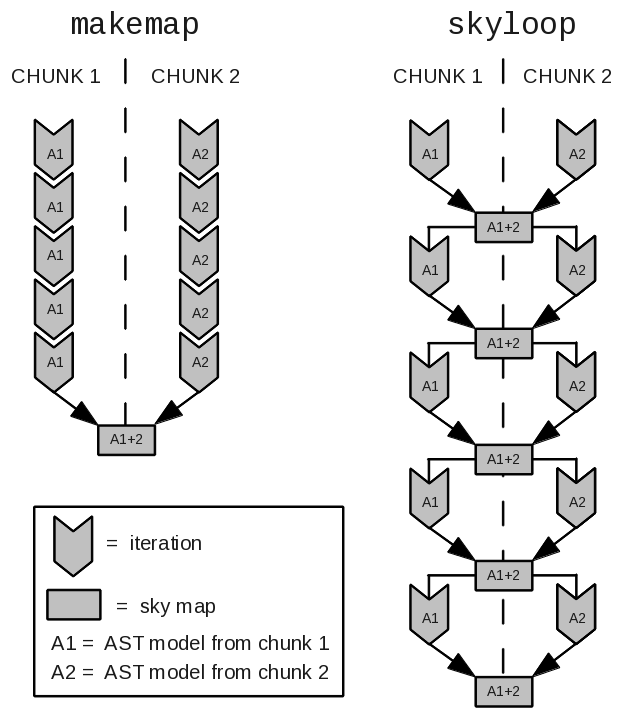
\includegraphics[width=0.55\linewidth]{sc21_skyloop}
  \caption{\small Illustration of the skyloop approach
  to map-making compared to the standard map-maker.
}
\label{fig:skyloop}
\end{figure}

Be aware that \texttt{skyloop} uses a lot of disk space. Setting
environment variable \texttt{STAR\_TEMP} to a suitable location
before you start will prevent \skyloop\ from crashing
if you run out of temporary storage space.
\begin{myquote}
\begin{verbatim}
% setenv STAR_TEMP .
\end{verbatim}
\end{myquote}
\texttt{skyloop} is then called in the same way as \makemap, with
 a configuration file specified on the command line.
\begin{myquote}
\begin{verbatim}
% skyloop in=^myfiles.lis out=map_skyloop config=^dimmconfig_bright_extended.lis \
LOGFILE=skyloop.log ILEVEL=ATASK GLEVEL=debug
\end{verbatim}
\end{myquote}

\subsection{Troubleshooting}
\begin{latexonly}
\begin{table}[h!]
\begin{center}
\begin{tabular}{|p{5cm}|p{10.5cm}|}
\hline
\textbf{PROBLEM} & \textbf{POSSIBLE SOLUTION}\\
\hline
I have blobs in my map that look like thumbprints. & Try including
\texttt{dimmconfig\_fix\_blobs.lis} parameters:
\begin{itemize}[noitemsep]
  \item \param{flt.filt\_order~=~4} to set a 4th-order Butterworth filter for
  the \texttt{FLT} model.
  \item \param{flt.ring\_box1~=~0.5} uses a filter to identify and flag
  time-samples that are ringing after the \texttt{FLT} model. This only starts
  after the \param{ast.skip} iterations (in bright\_extended) have completed.
  \item \param{com.sig\_limit~=~2.5} flags time slices where the
  \texttt{COM} model is very different from the average for each
  subarray. Should only be used when \param{flt.filt\_order} is set. If
  set too stringently it can throw out a lot of data so modify with
  caution. An extremely conservative value would be 5.
\end{itemize}
In addition, check you are not using \param{flt.notfirst~=~1} as this
can make blobs worse.\\
\hline
I want to recover more extended structure. & There is a trade off
between extended emission and noise in your map. If you are willing to
accept more low frequency noise you can increase the filter scale with
\param{flt.filt\_edge\_largescale}. The default is 480\,arcsec but you
could try 600\,arcsec. To cosmetically reduce the increased background
noise you can set \param{flt.filt\_edge\_largescale\_last~=~200}. This
sets the background filtering to 200\,arcsec for the final iteration
only, though you can go as low as you want with it. \\
\hline
I want a flatter background.  & Try \param{com.perarray~=~1}, although
be aware this will lose structure on scales larger than a subarray. In
conjunction with \param{com.perarray~=~1} you can also use the
\param{ast.skip~=~8} parameter. This makes a map without subtracting an
\param{AST} model for the first eight iterations. If you are chasing
extended emission see the point above. \newline

For a cosmetic improvement in the background, set
\param{flt.filt\_edge\_largescale\_last} to a small value to get harsh
filtering on your final iteration.\\
\hline
I have linear striations in my map making my background look
scratchy.& Try setting \param{com.corr\_abstol~=~0.8} [default=0.2].
This rejects more bolometers with deviant common-mode signals.
However, as more bolometers are removed there are less data available
for you final map resulting in higher noise.\\
\hline
My map will not converge.& Try including \texttt{dimmconfig\_fix\_convergence.lis}
parameters:
\begin{itemize}[noitemsep]
\item \param{com.freeze\_flags~=~10}
\item \param{ast.zero\_freeze~=~10}
\item \param{flt.zero\_freeze~=~10}
\item \param{com.zero\_freeze~=~10}
\end{itemize}
Each of the these freeze parameters stop the masks growing after ten
iterations. By this stage the masks have essentially reached their
maximum scale but a few edge pixels oscillate in and out of the masks
preventing convergence.\\
\hline
\end{tabular}
\end{center}
\end{table}
\end{latexonly}

\begin{htmlonly}
\begin{table}[h!]
\begin{center}
\begin{tabular}{|l|l|}
\hline
\textbf{PROBLEM} & \textbf{POSSIBLE SOLUTION}\\
\hline
I have blobs in my map that look like thumbprints. & Try including
\texttt{dimmconfig\_fix\_blobs.lis} parameters:
\begin{itemize}
  \item \param{flt.filt\_order~=~4} to set a 4th-order Butterworth filter for
  the \texttt{FLT} model.
  \item \param{flt.ring\_box1~=~0.5} uses a filter to identify and flag
  time-samples that are ringing after the \texttt{FLT} model. This only starts
  after the \param{ast.skip} iterations (in bright\_extended) have completed.
  \item \param{com.sig\_limit~=~2.5} flags time slices where the
  \texttt{COM} model is very different from the average for each
  subarray. Should only be used when \param{flt.filt\_order} is set. If
  set too stringently it can throw out a lot of data so modify with
  caution. An extremely conservative value would be 5.
\end{itemize}
In addition, check you are not using \param{flt.notfirst~=~1} as this
can make blobs worse.\\
\hline
I want to recover more extended structure. & There is a trade off
between extended emission and noise in your map. If you are willing to
accept more low frequency noise you can increase the filter scale with
\param{flt.filt\_edge\_largescale}. The default is 480\,arcsec but you
could try 600\,arcsec. To cosmetically reduce the increased background
noise you can set \param{flt.filt\_edge\_largescale\_last~=~200}. This
sets the background filtering to 200\,arcsec for the final iteration
only, though you can go as low as you want with it. \\
\hline
I want a flatter background.  & Try \param{com.perarray~=~1}, although
be aware this will lose structure on scales larger than a subarray. In
conjunction with \param{com.perarray~=~1} you can also use the
\param{ast.skip~=~8} parameter. This makes a map without subtracting an
\param{AST} model for the first eight iterations. If you are chasing
extended emission see the point above. \newline

For a cosmetic improvement in the background, set
\param{flt.filt\_edge\_largescale\_last} to a small value to get harsh
filtering on your final iteration.\\
\hline
I have linear striations in my map making my background look
scratchy.& Try setting \param{com.corr\_abstol~=~0.8} [default=0.2].
This rejects more bolometers with deviant common-mode signals.
However, as more bolometers are removed there are less data available
for you final map resulting in higher noise.\\
\hline
My map will not converge.& Try including \texttt{dimmconfig\_fix\_convergence.lis}
parameters:
\begin{itemize}
\item \param{com.freeze\_flags~=~10}
\item \param{ast.zero\_freeze~=~10}
\item \param{flt.zero\_freeze~=~10}
\item \param{com.zero\_freeze~=~10}
\end{itemize}
Each of the these freeze parameters stop the masks growing after ten
iterations. By this stage the masks have essentially reached their
maximum scale but a few edge pixels oscillate in and out of the masks
preventing convergence.\\
\hline
\end{tabular}
\end{center}
\end{table}
\end{htmlonly}


\clearpage
\section{\xlabel{Examples}Examples of Different Reductions}
\label{sec:eg}

\subsection{\xlabel{Cosmology}Deep point-source maps}
\label{sec:cosmology}

The science goal of many extra-galactic SCUBA-2 observations is to
detect unresolved point sources. In the examples below we work through the
reduction of just such an extra-galactic field, A1835.

Most extra-galactic objects are on average only slightly brighter than
the confusion limit---the fluctuations of the background sky
brightness due to multiple super-imposed, unresolved sources within
the telescope beam, below which individual sources cannot be detected.
It is likely that any sources in the map will be at best, only a few
standard deviations brighter than the noise in the map (caused by a
combination of instrumental noise and source confusion).

The recommended reduction method for maps like these follow two main
steps---running the data through the map-maker using the
\texttt{dimmconfig\_blank\_field.lis} recipe (see
\cref{Section}{sec:config}{Specialised configuration files}). Then
applying the \picard\ \drrecipe{SCUBA2\_MATCHED\_FILTER} recipe (see
\cref{Section}{sec:mf}{Point-source extraction}).
\\ \\
\textbf{Step 1: Running the map-maker}
\vspace{0.2cm}\\
In this example the raw data is stored locally in a directory called
\texttt{data}. We have three observations (\#13, \#18, \#21) of the field
which we will reduced independently.

\begin{myquote}
\begin{verbatim}
% makemap data/s8*00013_00\*.sdf cosmo1 method=iterate \
config=^$STARLINK_DIR/share/smurf/dimmconfig_blank_field.lis

% makemap data/s8*00018_00\*.sdf cosmo2 method=iterate \
config=^$STARLINK_DIR/share/smurf/dimmconfig_blank_field.lis

% makemap data/s8*00021_00\*.sdf cosmo3 method=iterate \
config=^$STARLINK_DIR/share/smurf/dimmconfig_blank_field.lis

\end{verbatim}
\end{myquote}

\textbf{Step 2: Combining the maps}
\vspace{0.2cm}\\
These three maps are then combined using the \textsc{Picard} recipe
\xref{\drrecipe{MOSAIC\_JCMT\_IMAGES}}{sun265}{MOSAIC_JCMT_IMAGES}. In
this case we accept the default of \wcsmosaic\ mosaicking and
nearest-neighbour pixel spreading and so do not supply a parameter
file.
\begin{myquote}
\begin{verbatim}
% picard MOSAIC_JCMT_IMAGES cosmo*.sdf
\end{verbatim}
\end{myquote}
The output map, \texttt{cosmo2\_mos.sdf}, is shown in the left-hand
panel of \cref{Figure}{fig:cosmomap}{the figure below}. The advantage of using the
\textsc{Picard} recipe over standalone \Kappa\ commands is that the exposure
time is also propagated correctly to the output mosaic (it is stored
in the \texttt{MORE.SMURF.EXP\_TIME} extension).
\\

\myfigduo{sc21_850cosmo_bf}{sc21_850cosmo_mf_crop}{}{width=0.48\linewidth}{fig:cosmomap}{2mm}{
  Cosmology example: initial reduction and matched filter maps}{
  Reduced \textsc{pong} maps of cosmology field A1835. \textbf{Left:}
  Map reduced with \texttt{dimmconfig\_blank\_field.lis}.
  \textbf{Right:} Map on the left after the matched filter has been
  applied and it has been cropped.
}

\textbf{Step 3: Applying the matched filter}
\vspace{0.2cm}\\
In order to optimally find sources that are the size of the telescope
beam, we apply the matched filter recipe --
\xref{\drrecipe{SCUBA2\_MATCHED\_FILTER}}{sun265}{SCUBA2_MATCHED_FILTER}.
We create a simple parameter file called \texttt{smooth.ini}:
\begin{myquote}
\begin{verbatim}
[SCUBA2_MATCHED_FILTER]
SMOOTH_FWHM = 15
\end{verbatim}
\end{myquote}
where \texttt{SMOOTH\_FWHM~=~15} indicates that the background should be
estimated by first smoothing the map and PSF with a 15-arcsec FWHM
Gaussian. Next, the recipe is executed as follows:
%
\begin{myquote}
\begin{verbatim}
% picard -recpars smooth.ini SCUBA2_MATCHED_FILTER cosmo2_mos.sdf
\end{verbatim}
\end{myquote}
%
The output of this operation is a smoothed image called
\texttt{cosmo2\_mos\_mf.sdf} and a cropped version is shown in the
right-hand panel of \cref{Figure}{fig:cosmomap}{figure above}. You can immediately
see the contrast to the left-hand panel which is the output from the
map-maker. A number of signal peaks now emerge as possible sources.
\\ \\
\textbf{Step 4: Cropping the map}
\vspace{0.2cm}\\
Next we shall crop the map to remove the noisy edges,
in this case to a 900-arcsec radius circle. The output file will be named
\texttt{cosmo2\_mos\_mf\_crop.sdf}.
\begin{myquote}
\begin{verbatim}
% picard CROP_JCMT_IMAGES cosmo2_mos_mf.sdf

\end{verbatim}
\end{myquote}

\myfig{sc21_850cosmo_mf_crop_snr}{}{width=0.6\linewidth}{fig:snrmask}{
  Cosmology example: signal-to-noise map}{
  Signal-to-noise map made the \Kappa\ command \makesnr.
  The map has been scaled from 0 to $+$3.
}

\textbf{Step 5: Making a S/N map}
\vspace{0.2cm}\\
Finally, we need to find sources. The filtered map contains a
VARIANCE component, so it is easy to produce a S/N map using the
\textsc{Kappa} task \makesnr:
\begin{myquote}
\begin{verbatim}
% makesnr cosmo2_mos_mf_crop cosmo2_mos_mf_crop_snr
\end{verbatim}
\end{myquote}

The resulting map, \texttt{cosmo2\_mos\_mf\_snr}, is shown in
\cref{Figure}{fig:snrmask}{signal-to-noise image}. Compared with the
matched filter map the
edges no longer appear as noisy because they have been down-weighted
by the larger noise values where there were less data.
\\ \\
\textbf{Step 6: Identifying sources}
\vspace{0.2cm}\\
The basic procedure for identifying sources would be to locate peaks
above some threshold S/N. The S/N image above shows peaks that are
likely to be real sources. For a start, a source appears where
expected at the 0,0 position.

But how can we check if these sources are real?
\begin{itemize}

\item One option is to split your data into mutually exclusive subsets
  and produce independent maps. Are the highest S/N peaks detected in each of
  them?
\item A second test is to compare the number of \emph{negative} peaks above
  a given S/N with the number of \emph{positive} peaks.
\end{itemize}

\textbf{Note:} A \picard\ recipe dealing specifically with blank field
maps is under development. Follow the
\htmladdnormallink{\textit{Pipelines and Archives
blog}}{http://pipelinesandarchives.blogspot.com/}
\latex{\footnote{http://pipelinesandarchives.blogspot.com/}} for all
the latest updates and releases.

\subsection{\xlabel{Galactic}Extended galactic sources}
\label{sec:bright_ex}

This example is concerned with recovering bright extended emission.
The signal from extended emission varies slowly as seen by the array
passing over it. It thus appears at lower frequencies in the power
spectrum and complicates the high pass filter selection. Too harsh a
filter will make flat maps but any extended emission will have been
removed in doing so.
\\ \\
\textbf{Step 1: Running the map-maker}
\vspace{0.2cm}\\
We run the map-maker using \texttt{dimmconfig\_bright\_extended.lis};
we have also specified a couple of overrides on the command
line---\texttt{maptol}~=~0.04 is slightly more stringent than default and
\texttt{ast.zero\_snr}~=~3.5 constrains emission everything below
3.5\,$\sigma$ to zero.

In this example we give the map-maker a file containing a list of the
input files (filelist.txt) and
\texttt{dimmconfig\_bright\_extended.lis} is in the local directory.

\begin{myquote}
\begin{verbatim}
% makemap in=^filelist.txt 850galactic method=iterate \
config='"^dimmconfig_bright_extended.lis,maptol=0.04,ast.zero_snr=3.5"'
\end{verbatim}
\end{myquote}

\myfig{sc21_gal_11}{[t!]}{width=0.6\linewidth}{fig:galmakemap}{
  Galactic example: initial reduction using \texttt{dimmconfig\_bright\_extended.lis}}{
  The output from the map-maker using \texttt{dimmconfig\_bright\_extended.lis}.
}

\textbf{Step 2: Generating an external mask}
\vspace{0.2cm}\\
Next we create an external mask from the output of \makemap. Here we
follow the steps outlined in \cref{Section}{sec:mask}{Masking options}.

\begin{myquote}
\begin{verbatim}
% makesnr 850map 850map_snr
\end{verbatim}
\end{myquote}

This S/N map is thresholded to set everything below 3\,$\sigma$ to 0 and
everything above to 1.

\begin{myquote}
\begin{verbatim}
% thresh 850map_snr 850map_mask thrlo=3 newlo=0 thrhi=3 newhi=1
\end{verbatim}
\end{myquote}
The thresholded map is shown in the left-hand panel of
\cref{Figure}{fig:mask}{this figure}. The next step is to smooth this map
by convolving it with a Gaussian of 16\,arcsec. For this we use a factor
of 4 for the FWHM parameter.

\begin{myquote}
\begin{verbatim}
% gausmooth 850map_mask 850map_mask_sm fwhm=4
\end{verbatim}
\end{myquote}

We threshold the map again to produce our mask. In this case all
values below out threshold are set to `bad'. The the smoothed map now
has values scaled between 0 and 1, we set our threshold at 0.02 to
include more of the emission beyond the 3\,$\sigma$ edge.
\begin{myquote}
\begin{verbatim}
% thresh 850map_mask_sm 850map_mask_zm thrlo=0.02 newlo=bad thrhi=0.02 newhi=1
\end{verbatim}
\end{myquote}
The final mask is shown in the right-panel of \cref{Figure}{fig:mask}{this figure},
note how it encompasses more emission and has softer edges than the
first threshold map. \\

\myfigduo{sc21_gal_mask1}{sc21_gal_mask2}{[t]}{width=0.475\linewidth}{fig:mask}{2mm}{
  Galactic example: thresholded SNR map and smoothed map}{
  \textbf{(Left)} The initial mask created by thresholding 850map\_snr
  to 3$\sigma$. \textbf{(Right)} Second mask made by thresholding the
  smoothed map to 0.02.
}

\textbf{Step 3: Re-running the map-maker with an external mask supplied}
\vspace{0.2cm}\\
As a last step the map is re-made with this mask supplied as an external
file. For this run we apply the additional parameters in a
personalised configuration file, \texttt{mydimmconfig.lis}.
\begin{myquote}
\begin{verbatim}
% makemap in=^filelist.txt 850galactic method=iterate \
config=^mydimmconfig.lis ref=850map_mask_zm
\end{verbatim}
\end{myquote}

The configuration file, \texttt{mydimmconfig.lis}, has the following
format---note how it is based on
\texttt{dimmconfig\_bright\_extended.lis}. It has decreased the
convergence parameter to \texttt{MAPTOL}=0.03 but increased the number
of iterations to compensate as 40 is unlikely to be sufficient.
\begin{myquote}
\begin{verbatim}
^$STARLINK_DIR/share/smurf/dimmconfig_bright_extended.lis
numiter = -100
noisecliphigh = 10.0
maptol = 0.03
ast.zero_mask=1
ast.zero_snr = 0
\end{verbatim}
\end{myquote}

\textbf{Step 4: Cropping the map}
\vspace{0.2cm}\\
We can now crop the map to remove the noisy edges using the \picard\ recipe
\drrecipe{CROP\_JCMT\_IMAGES}. To determine what to trim we can look
at the exposure-time image with \gaia.

\myfig{sc21_gal_exptime}{[th!]}{width=0.7\linewidth}{fig:exptime}{
  Galactic example: exposure time map}{
  The exposure-time image of the science map from \cref{Figure}{fig:galmakemap}{
  our example map}. You can right-click and drag the mouse
  between two points to measure the distance. Here we see the exposure
  time dropping off sharply at a radius of 30\,arcmin. A non-default
  colour scale has been chosen to illustrate the morphology.
}

\cref{Figure}{fig:exptime}{The exposure-time image} shows a sharp drop
off at a radius of 30\,arcmin. We can thus specify a parameter file like so:
\begin{center}
\begin{myquote}
\begin{verbatim}
[CROP_JCMT_IMAGES]
MAP_RADIUS = 1800
\end{verbatim}
\end{myquote}
\end{center}

\begin{myquote}
\begin{verbatim}
% picard CROP_JCMT_IMAGES 850galactic.sdf
\end{verbatim}
\end{myquote}
The final cropped map is shown in \cref{Figure}{fig:crop_map}{this plot}. Compared
with the first map out of the map-maker
(\cref{Figure}{fig:galmakemap}{first map}),
slightly more of the faint extended emission is apparent.

One of the challenges facing this type of reduction is the need to
account for both faint extended structure and very bright sources in
the same map. You may find some degree of bowling remains around the
brightest sources.

A patchy looking background is a result of the more relaxed high pass
filtering and is an inevitable consequence of recovering extended
emission. To remove that is to also remove extended emission as they
are essentially indistinguishable.

There are areas you may wish to experiment with. One is to adjust the
filtering---see \cref{Section}{sec:tweak}{Tweaking the configuration
file} for details. Another option is to supply an external mask from
a different dataset, e.g. a
\htmladdnormallink{Herschel}{http://herschel.esac.esa.int/} map.

\myfig{sc21_gal12_crop}{[t!]}{width=0.8\hsize}{fig:crop_map}{
  Galactic example: cropped final map}{
  The final cropped, reduced map from the map-maker run with
  an external mask supplied.
}


\clearpage
\section{\xlabel{pipeline}The SCUBA-2 Pipeline}
\label{sec:pipe}

\subsection{\xlabel{pl_overview}Pipeline overview}

SCUBA-2 data reduction pipelines have been developed based on the
existing \oracdr\ pipeline (Cavanagh et al., 2008\cite{oracdr}) used
for ACSIS. There are three distinct pipelines currently utilised by
SCUBA-2: two of these, the quick-look (QL) and summit pipelines, are
run in real time at the JCMT during data acquisition; the third, the science
pipeline, offers a comprehensive reduction, which users can run locally.

\begin{itemize}
\item The QL runs quality assurance checks on the data as it comes in.
For science data it calculates the noise between 2\,Hz and 10\,Hz,
along with the NEP and effective NEP, for each 30-second scan. These
values undergo quality-assurance checks to ensure SCUBA-2 is within
an acceptable operating range.
\item The summit pipeline is designed to provide a quick map of the
data, it does this by running fewer iterations and chunking the data
more. This is a useful guide to observers who wish to check the
quality of their data.
\item The science pipeline is run the following day. Data from the
previous night is processed using an optimal reduction routine, that
includes the map-maker and a number of post-processing steps (outlined
below). These data are transferred to CADC and available for download
by project members the following day.
\end{itemize}

The manual for the SCUBA-2 pipeline can be found at \pipelinesun,
while the pipeline software comes as part of the \starlink\ suite.


\subsection{\xlabel{science_pl}The Science Pipeline}

The science pipeline will automate many of the steps discussed in
\cref{Section}{sec:maps}{Reducing your data}:
\vspace{-0.3cm}
\begin{itemize}\itemsep-0.3em
\item Run the iterative map-maker.
\item Apply the FCF to calibrate to mJy/beam.
\item Co-add multiple observations of the same object.
\item Apply the matched-filter (blank-field configuration file only)
\item Run a source finding algorithm.
\end{itemize}

\subsection{\xlabel{pl_output}Pipeline recipes}
\label{sec:recipes}

When MSBs are created, the PI can select a pipeline recipe to assign
to the data. When the data is run through the science pipeline this
recipe is used by default. This recipe can overridden on the command
line---see \cref{Section}{sec:parameterfile}{Changing the defaults}.

Described below are the five main \oracdr\ science recipes.

\subsection{\xlabel{extsources}REDUCE\_SCAN}
\vspace{-0.3cm}
\textbullet\ Configuration file: \texttt{dimmconfig.lis}

This recipe uses the default configuration file for \makemap, unless
the sources is identified as a calibrator. After all observations have
been processed the data is co-added and calibrated using the default
FCF.  The noise and NEFD properties for the co-add are calculated and
written to log files (\texttt{log.noise} and \texttt{log.nefd}
respectively). Finally, the \cupid\ task \findclumps\ is run using the
FellWalker algorithm to create a source catalogue.

For calibrators, \texttt{dimmconfig\_bright\_compact.lis} is used and
FCFs are derived from the map.


\subsubsection{\xlabel{extsources}REDUCE\_SCAN\_CHECKRMS}
\vspace{-0.3cm}
\textbullet\  Configuration file = \texttt{dimmconfig.lis}

This recipe is the same as \drrecipe{REDUCE\_SCAN}, but includes extra
performance estimations determined by \drrecipe{SCUBA2\_CHECK\_RMS} (see
\cref{Section}{sec:checkrms}{Getting the noise}). These extra metrics
are written to a log file log.checkrms. The advantage of running
\drrecipe{SCUBA2\_CHECK\_RMS} in the pipeline rather than as a standalone
\picard\ recipe is that is able to calculate results for co-added
files.

\subsubsection{\xlabel{extsources}REDUCE\_SCAN\_EXTENDED\_SOURCES}
\vspace{-0.3cm}
\textbullet\  Configuration file = \texttt{dimmconfig\_bright\_extended.lis}

This is the recipe for processing extended sources, with the
\texttt{dimmconfig\_bright\_extended.lis} configuration file called by
\makemap. Multiple observations are co-added and the output
map is calibrated in units of mJy/arcsec$^2$. This recipe also
performs a source finder routine; the results are written as a FITS
catalogue (with file extension \texttt{.FIT}) which can be read as a
local catalogue into \gaia.

\subsubsection{\xlabel{faint}REDUCE\_SCAN\_FAINT\_POINT\_SOURCES}
\vspace{-0.3cm}
\textbullet\  Configuration file = \texttt{dimmconfig\_blank\_field.lis}

This is the recipe for processing maps containing faint compact
sources. This time the configuration file called by \makemap\
is \texttt{dimmconfig\_blank\_field.lis}. The resulting map is further
processed with a matched filter to give the first output map. Then the
S/N is taken to enhance point sources, this
S/N map is written out as a second output file. This
recipe also performs a source finder routine; the results are written
as a FITS catalogue (with file extension \texttt{.FIT}) which can be
read as a local catalogue into \gaia.

\subsubsection{\xlabel{faintjk}FAINT\_POINT\_SOURCES\_JACKKNIFE}
\vspace{-0.3cm}
\textbullet\  Configuration file = \texttt{dimmconfig\_blank\_field.lis}

This recipe uses a jack-knife method to remove residual low-spatial
frequency noise and create an optimal matched-filtered output map. The
map-maker is run twice, first as a standard reduction using
\texttt{dimmconfig\_blank\_field.lis}, and the second time with a fake
source added to the time series. This creates a signal map and an
effective PSF map. A jack-knife map is generated from two halves of
the dataset and the maps are `whitened' by the removal of the residual
1/\emph{f} noise. The whitened signal map is processed with the
matched filter using the whitened PSF map as the PSF input. The data
are calibrated in mJy/beam using a corrected FCF. See
\cref{Section}{sec:jk}{Example 2 - Advanced pipeline method} for a
more-detailed description of this recipe and the files produced.

\section{Changing the defaults}
\label{sec:parameterfile}
\subsection{Changing the pipeline recipe}
You can override the recipe set in the header by listing any different
one on the command line when starting \oracdr. For example
\begin{myquote}
\begin{verbatim}
% oracdr -file mylist -loop file -log x REDUCE_SCAN_CHECKRMS
\end{verbatim}
\end{myquote}

You can find out which recipe is set in the data header via the FITS
header \texttt{RECIPE} parameter in any of your raw files.  For
example both of these options will return the same result:
\begin{myquote}
\begin{verbatim}
% fitsval s8a20120725_00045_0003.sdf RECIPE
% fitslist s8a20120725_00045_0003.sdf | grep RECIPE
\end{verbatim}
\end{myquote}

\subsection{Changing the configuration file}

Although each recipe calls one of the standard configuration files the
user can specify their own. You will need to create a recipe parameter
file. This file will contain set the parameter \param{MAKEMAP\_CONFIG} to be
your new configuration file. This must be preceded by the recipe name
used in the reduction.

For example, to run the pipeline with \drrecipe{REDUCE\_SCAN\_CHECKRMS} but your
own configuration file (\texttt{myconfig.lis}), the recipe parameter file
(named \texttt{mypars.ini}) will look like this:
\vspace{0.2cm}
\begin{myquote}
\begin{verbatim}
[REDUCE_SCAN_CHECKRMS]
MAKEMAP_CONFIG = myconfig.lis
\end{verbatim}
\end{myquote}
\vspace{0.4cm}
Then run the pipeline calling the parameter file via the
\texttt{-recpars} option.
\begin{myquote}
\begin{verbatim}
% oracdr -file mylist -loop file -log x -recpars=myparams.ini REDUCE_SCAN_CHECKRMS
\end{verbatim}
\end{myquote}


\subsection{\xlabel{running_pl}Running the Science Pipeline}
\label{sec:plsteps}

\begin{minipage}[t]{0.15\linewidth}
\textbf{Step 1:}
\end{minipage}
\begin{minipage}[t]{0.85\linewidth}
\textbf{Initialise ORAC-DR} \\This is simply done by:
\begin{myquote}
\begin{verbatim}
% oracdr_scuba2_850 -cwd
\end{verbatim}
\end{myquote}
\end{minipage}

\begin{minipage}[t]{0.15\linewidth}
\textbf{Step 2:}
\end{minipage}
\begin{minipage}[t]{0.85\linewidth}
\textbf{Set environment variables}. \\These ensure the data are read
from and written to the right places. Many are set automatically when
the pipeline is initialised but others must be set manually. Details
of the optional variables are given in \pipelinesun\ but the three
main ones are:
\begin{itemize}\itemsep-0.1em
\item \param{STARLINK\_DIR}: Location of your Starlink installation.
\item \param{ORAC\_DATA\_IN}: The location where the data should be read from.
If you are supplying a text file listing the raw data this should be the
location of that file.
\item \param{ORAC\_DATA\_OUT}: The location where the data products should be
written. Also used as the location for a user-specified configuration file.\\
\end{itemize}
\end{minipage}

\begin{minipage}[t]{0.15\linewidth}
\textbf{Step 3:}
\end{minipage}
\begin{minipage}[t]{0.85\linewidth}
\textbf{(Optional) Create your personalised configuration file and/or parameter file.} \\
See \cref{Section}{sec:parameterfile}{Changing the defaults} for
details. In this example we check the \param{RECIPE} parameter and find the
recipe \drrecipe{REDUCE\_SCAN} is assigned to our data. We are happy with the
steps in this recipe but want to supply a new configuration file. To
do so we create a parameter file called \texttt{mypars.ini}.\\*

\end{minipage}


\begin{minipage}[t]{0.15\linewidth}
\textbf{Step 4:}
\end{minipage}
\begin{minipage}[t]{0.85\linewidth}
\textbf{Run the pipeline.} \\Run the pipeline using the
\texttt{-recpars} option to specify a parameter file if required.
\begin{myquote}
\begin{verbatim}
% oracdr -loop file -files inputlist.txt -log xf -recpars mypars.ini
\end{verbatim}
\end{myquote}
\end{minipage}


\subsection{\xlabel{pl_output}Pipeline output}

The pipeline will produce a group file for each object being
processed. If the pipeline is given data from multiple nights, all
those data will be included in the group co-add using inverse variance
weighting.

The final maps in your output directory will have the suffix
\texttt{\_reduced}. Maps will be made for individual observations,
which will start with an \texttt{s} (e.g.
\texttt{s20120720\_00030\_850\_reduced.sdf}). Group maps, which may contain
co-added observations from a single night, are also produced which
have the prefix \texttt{gs} (e.g. \texttt{gs20120720\_30\_850\_reduced.sdf}).

\textbf{Note:} A group file is \emph{always} created, even if only a single
observation is being processed.

Additionally, PNG images are made of the reduced files at a variety of
resolutions.

\subsubsection{\xlabel{cadc}Getting your data from CADC}

The JCMT Science Archive is hosted by The Canadian Astronomy Data
Centre (CADC). Both raw data and data processed by the science pipeline
are made available to PIs and co-Is through the CADC interface
(\texttt{http://www3.cadc-ccda.hia-iha.nrc-cnrc.gc.ca/jcmt/}).

To access proprietary data you will need to have your CADC username
registered by the JAC and thereby associated with the project code.

An important search option to be aware of is `Group Type', where your
options are Simple, Night, Project and Public. Simple (which becomes
`obs' on the result page) is an individual observation; night means
the group file from the pipeline (these may or may not include more
than one observation; the `Group Members' value will tell you), the
project option is generated if an entire project has been run through
the pipeline and identical sources across the project are co-added
into master group files.

\clearpage

\begin{thebibliography}{}
\addcontentsline{toc}{section}{References}

\bibitem{archibald}
Archibald,~E.~N., et~al, 2002, \htmladdnormallink{\textit{On the atmospheric limitations
of ground-based submillimetre astronomy using array receivers}}{
http://dx.doi.org/10.1046/j.1365-8711.2002.05582.x}, MNRAS, 336, 1-13
(DOI:10.1046/j.1365-8711.2002.05582.x)

\bibitem{oracdr}
Cavanagh~B., Jenness~T., Economou~F., Currie~M.~J., 2008,
\htmladdnormallink{\textit{The ORAC-DR data reduction
pipeline}}{http://dx.doi.org/10.1002/asna.200710944}, Astron. Nactr., 329, 295
(DOI:10.1002/asna.200710944)

\bibitem{smurf}
Chapin~E.~L., et~al., 2013, \textit{SMURF -- Sub-Millimetre User Reduction
Facility}, \xref{Starlink User Note 258}{sun258}{}

\bibitem{mapmaker}
Chapin~E.~L., et~al., 2013, \textit{SCUBA-2: iterative map-making with the
Sub-Millimetre User Reduction Facility} MNRAS,
\htmladdnormallink{accepted}{http://arxiv.org/abs/1301.3652}

\bibitem{ssds}
Currie~M.~J., Wallace~P.~T., Warren-Smith~R.~F., 1989,
\textit{Starlink Standard Data Structures}, \xref{Starlink General
Paper 38.2}{sgp38}{}

\bibitem{kappa}
Currie~M.~J., Berry~D.~S, 2013, \textit{KAPPA -- Kernel Application Package},
\xref{Starlink User Note 95}{sun95}{}

\bibitem{dempsey12}
Dempsey~J.~T. et al., 2013, \textit{SCUBA-2: on-sky calibration using
submillimetre standard sources}, MNRAS,
\htmladdnormallink{accepted}{http://arxiv.org/abs/1301.3773}

\bibitem{dempsey-spie}
Dempsey~J.~T., Friberg~P., Jenness~T., Bintley~D., Holland~W.~S., 2010
\htmladdnormallink{\textit{Extinction correction and on-sky calibration of
SCUBA-2}}{http://dx.doi.org/10.1117/12.856476},
Proc.\ SPIE, 7741 (DOI:10.1117/12.856476)

\bibitem{gaia}
Draper~P.~W., Gray~N., Berry~D.~S., Taylor~M., 2012,
\textit{GAIA -- Graphical Astronomy and Image Analysis Tool},
\xref{Starlink User Note 214}{sun214}{}

\bibitem{picard}
Gibb~A.~G., Jenness~T., Economou~F., 2012, \textit{PICARD --- a
PIpeline for Combining and Analyzing Reduced Data}
\xref{Starlink User Note 265}{sun265}{}

\bibitem{s2main}
Holland, W. S., et~al, 2013, \textit{SCUBA-2: The 10,000 pixel bolometer
camera on the James Clerk Maxwell Telescope}, MNRAS,
\htmladdnormallink{accepted}{http://arxiv.org/abs/1301.3650}

\bibitem{flux1}
Jenness~T., et~al, 2002, \htmladdnormallink{\textit{Towards the automated
reduction and calibration of SCUBA data from the James Clerk Maxwell
Telescope}}{http://dx.doi.org/10.1046/j.1365-8711.2002.05604.x},
MNRAS, 336, 14-21 (DOI:10.1046/j.1365-8711.2002.05604.x)

\bibitem{sc2ana005}
Scott~D., Van Engelen~A., 2005, \htmladdnormallink{\textit{Scan Mode Strategies for
SCUBA-2}}{http://docs.jach.hawaii.edu/JCMT/SC2/ANA/S210/005/sc2_ana_s210_005.ps},
SCUBA-2 Data Reduction document SC2/ANA/S210/005

\end{thebibliography}

\newpage
\appendix
\section{\xlabel{app_clean}Cleaning the Raw Data}
\label{app:clean}

You can use the \smurf\ task \clean\ to help inspect time-series.
\task{sc2clean} can be used to do two basic tasks in one go: concatenate data
(with or without applying a flatfield); and cleaning (fix up steps and
spikes, remove the means, filter, remove common-mode etc.). It uses
the same configuration files as the iterative map-maker (though
ignoring the map-making specific items).

In this first basic example, we just want to clean up some data enough
to see whether the bolometers have been flat-fielded correctly, and
more-or-less exhibit the same behaviour over time. The pre-processing
or cleaning steps used by the default configuration file are
summarised in \cref{Table}{tab:dimmdef}{this table}.

\begin{myquote}
\begin{verbatim}
% sc2clean $FILES clean config=^$STARLINK_DIR/share/smurf/dimmconfig.lis
\end{verbatim}
\end{myquote}

Here \texttt{\$FILES} can just be a single file from a subarray, or a
subset, e.g. \texttt{s8a20110417\_00051\_0003.sdf} (the first file
containing science data), \texttt{s8a20110417\_00051\_000"[1234]"}
(file 1 is a noise observation with shutter closed that gets ignored,
file 2 is a flatfield observation that will be used to override the
flatfield stored in the subsequent files 3 and 4 which are
concatenated together, the \texttt{.sdf} is optional),
\texttt{s8a20110417\_00051\_000\textbackslash?} (files 1 through 9),
\texttt{s8a20110417\_00051\_\textbackslash*} (the whole observation).

If you inspect the resulting \texttt{clean.sdf} in \gaia\
(\cref{Section}{sec:gaiacube}{Displaying time-series data}) and flip
through the data cube you should
see all of the bolometers signals go up and down together with about
the same amplitude: the hope is that for a well-behaved instrument you
are mostly seeing sky noise variations that are seen with roughly the
same amplitude by all bolometers.

Another common feature, if the scans are particularly long and/or fast
(e.g. 1\,degree across), is strong periodic signals that are correlated
with the scan pattern. See \cref{Section}{sec:scan}{Displaying scan
patterns}---in particular
you will want to plot \texttt{az} and \texttt{el} (the absolute
azimuth and elevation), and also \texttt{daz} and \texttt{del} (the
azimuth and elevation offsets from the map centre). This signal is
usually azimuth-correlated due to magnetic field pickup. It only shows
up in azimuth, because the instrument is on a Nasmyth platform and
therefore does not move in elevation.

Part of the reason the signals look the same is because they have been
flatfielded. You can turn off flatfielding using the \texttt{noflat}
option to \task{sc2clean}, and you should then see that all of the detector
amplitudes vary.

Another very useful option is to remove the common signal observed by
all of the bolometers. This may be accomplished by

\begin{myquote}
\begin{verbatim}
% sc2clean $FILES clean \
   config='"^$STARLINK_DIR/share/smurf/dimmconfig.lis,compreprocess=1"'
\end{verbatim}
\end{myquote}

The residual of this signal will exhibit second-order time-varying
correlated signals across the focal plane. Usually these are not very
large, but in some cases some very large localized signals have been
detected, particularly in the 850\,$\mu$m arrays in early 2011.

Another variation on this is to accentuate the residual low-frequency
noise by low-pass filtering the result. This can again be accomplished
by simply adding a filter command in the \texttt{config} parameter,
which in this case low-pass filters with a cutoff at 10\,Hz:

\begin{myquote}
\begin{verbatim}
% sc2clean $FILES clean \
config='"^$STARLINK_DIR/share/smurf/dimmconfig.lis,compreprocess=1,filt_edgelow=10"'
\end{verbatim}
\end{myquote}

Finally, in some cases you might just want to fit and remove
polynomial baselines from the bolometers (by default only the mean is
removed). This example will remove a line, but you can increase the
value of \texttt{order} to remove higher-order polynomials

\begin{myquote}
\begin{verbatim}
% sc2clean $FILES clean \
   config='"^$STARLINK_DIR/share/smurf/dimmconfig.lis,order=1"'
\end{verbatim}
\end{myquote}

Any of the cleaning parameter can be specified independently of the
default configuration files like so:
\begin{myquote}
\begin{verbatim}
% sc2clean $FILES clean config='"order=1,dcfitbox=30,dcthresh=25,dcsmooth=50"'
\end{verbatim}
\end{myquote}
Or you can create your own customised configuration file. All the
pre-processing options that may be specified are listed and described
in \texttt{dimmconfig.lis}---see \cref{Appendix}{app:dimm}{here}.


\newpage
\section{\xlabel{calib}SCUBA-2 Data Calibration}
\label{app:cal}

\subsection{\xlabel{fcf}Flux conversion factors (FCF)}
\label{app:fcf}

Primary and secondary calibrator observations have been reduced using
the specifically designed \texttt{dimmconfig\_bright\_compact.lis}.
The maps produced from this are then analysed using tailor-made
\picard\ recipes. For instructions on applying the FCFs to your map see
\cref{Section}{sec:cmult}{this page}.

A map reduced by the map-maker has units of pW. To calibrate the data
into units of janskys (Jy), a set of bright, point-source objects with
well known flux densities are observed regularly to provide a flux
conversion factor (FCF). The data (in pW) can be multiplied by this FCF
to obtain a calibrated map. The FCF can also be used to assess the
relative performance of the instrument from night to night. The noise
equivalent flux density (NEFD) is a measure of the instrument
sensitivity, and while not discussed here, is also produced by the
\textsc{Picard} recipe shown here. For calibration of primary and secondary
calibrators, the FCFs and NEFDs have been calculated as follows:

\begin{enumerate}
\item{The \textsc{Picard} recipe \drrecipe{SCUBA2\_FCFNEFD} takes the reduced
map, crops it, and runs background removal. Surface-fitting
parameters are changeable in the \textsc{Picard} parameter file.}
\item{It then runs the \Kappa\ \beamfit\ task on the specified point
source. The \task{beamfit} task will estimate the peak (uncalibrated)
flux density and the FWHM. The integrated flux density within a
given aperture (30-arcsec radius default) is calculated using
\photom\ \autophotom. Flux densities for calibrators such as Uranus,
Mars, CRL~618, CRL~2688 and HL~Tau are already known to
\picard. To derive an FCF for other sources of known flux densities,
the fluxes can be added to the parameter file with the source name
(in upper case, spaces removed): \texttt{FLUX\_450.MYSRC~=~0.050}
and \texttt{FLUX\_850.MYSRC~=~0.005} (where the values are in Jy),
for example.}

\item {Three alternative FCF values are calculated, two of which are
described below.}
\end{enumerate}

\begin{itemize}

\item{\textbf{\fcfa}}

\begin{equation}
\label{eq:fcf_arcsec}
\mathrm{FCF_{arcsec}} = \frac{S_\mathrm{tot}}{P_\mathrm{int} \times
A_\mathrm{pix}}
\end{equation}

where $S_\mathrm{tot}$ is the total flux density of the calibrator,
$P_\mathrm{int}$ is the integrated sum of the source in the map (in
pW) and $A_\mathrm{pix}$ is the pixel area in arcsec$^2$, producing an
FCF in Jy/arcsec$^2$/pW.

\item{\textbf{\fcfb}}

\begin{equation}
\label{eq:fcf_beam}
\mathrm{FCF_{beam}} = \frac{S_\mathrm{{peak}}}{P_\mathrm{peak}}
\end{equation}
producing an FCF in units of Jy/beam/pW.
\end{itemize}

The measured peak signal here is derived from the Gaussian fit of
\beamfit. The peak value is susceptible to pointing and focus errors,
and we have found this number to be somewhat unreliable, particularly
at 450$\mu$m.


\subsection{\xlabel{extinction}Extinction correction}

Analysis of the SCUBA-2 secondary calibrators has allowed calculation
of the transmission relationships for the SCUBA-2 450\,$\mu$m and
850\,$\mu$m pass-bands to be determined. Full details of the analysis
and on-sky calibration methods of SCUBA-2 can be found in Dempsey et
al.\ (2013)~\cite{dempsey12}\cite{dempsey-spie}.

Archibald et al. (2002)\,\cite{archibald} describes how the Caltech
Submillimeter Observatory (CSO) 225\,GHz opacity, $\tau_{225}$,
relates to SCUBA opacity terms in each band, $\tau_{450}$ and
$\tau_{850}$. The JCMT water-vapour radiometer (WVM) uses the 183\,GHz
water line to calculate the precipitable water vapour (PWV) along the
line-of-sight of the telescope. This PWV is then input into an
atmospheric model to calculate the zenith opacity at 225\,GHz
($\tau_{225}$). This allows ease of comparison with the adjacent CSO
225\,GHz tipping radiometer. The opacities have been as:

\begin{equation}
\tau_{450} = 26.0 \times (\tau_{225} - 0.012);
\end{equation}
and
\begin{equation}
\tau_{850} = 4.6 \times (\tau_{225} - 0.0043).
\end{equation}

The SCUBA-2 filter characteristics are described in
detail \htmladdnormallinkfoot{on the JCMT
website}{http://www.jach.hawaii.edu/JCMT/continuum/scuba2/filter/}.

The extinction correction parameters that scale from $\tau_{225}$ to
the relevant filter have been added to the map-maker code. You can
override these values by setting \param{ext.taurelation.filtname} in
your map-maker config files to the two coefficients `($a$,$b$)' that you
want to use (where \texttt{filtname} is the name of the filter). The
defaults are listed in \texttt{\$SMURF\_DIR/smurf\_extinction.def}.
%It is worth noting that if an individual science map and corresponding calibrator observation has already been reduced with the old factors (and your source and calibrator are at about the same airmass and if the tau did not change appreciably), any errors in extinction correction should cancel out in the calibration.

\newpage
\section{\xlabel{calcrms}SCUBA2\_CHECK\_RMS}
\label{app:checkrmsparams}

\begin{latexonly}
\begin{table}[h!]
\begin{center}
\begin{tabular}{|p{2.5cm}|p{12cm}|}
\hline
\textbf{Parameter} & \textbf{Description}\\
\hline
    UT & UT date including day fraction\\
    Source & object name, upper case with spaces removed\\
    Obs & observation number\\
    FILTER & filter (wavelength)\\
    telapsed & elapsed time of observation in seconds\\
    texp & mean exposure time, derived from EXP\_TIME NDF component (sec)\\
    trans & mean line-of-sight transmission\\
    nep\_av & mean NEP for current observation (W/sqrt(Hz))\\
    nep\_av\_err & uncertainty in nep\_av (W/sqrt(Hz))\\
    rms\_nep & RMS derived from nefd\_nep (mJy/beam)\\
    nefd\_nep & NEFD derived from nep\_av and scaled elapsed time (mJy sqrt(sec))\\
    rms\_map & RMS noise in map, obtained from median of error component (mJy/beam)\\
    nefd\_map & NEFD derived from combination of variance and exposure time images (mJy sqrt(sec))\\
    rms\_itc & RMS noise estimated by SCUBA-2 integration time calculator (ITC) (mJy/beam) *\\
    nefd\_itc & NEFD derived from rms\_itc and scaled elapsed time (mJy sqrt(sec)) *\\
    itc\_obstype & observation type used by the ITC to derived RMS\\
    rms\_ratio & ratio of rms\_map to rms\_itc\\
    El & mean elevation in degrees\\
    CSO & mean zenith optical depth at 225 GHz, derived from WVM\\
    Tau & mean zenith optical depth at the current wavelength (given by FILTER above)\\
    Radius & radius in arcsec of image used in analysis\\
    pixscale & pixel scale in arcsec\\
    f & ITC f parameter\\
    project & project ID\\
\hline
\end{tabular}
\end{center}
\end{table}
\end{latexonly}
Some values (the Noise Equivalent Power values) need to be calculated
from the raw data. Recall the NEP corresponds to the noise in the raw
data and is a combination of instrument and atmospheric noise.

\newpage
\section{\xlabel{matchedfilter}SCUBA-2 Matched Filter}
\label{app:mf}

In order to optimally find sources that are the size of the telescope
beam, and suppress this residual large-scale noise, the \picard\
recipe \drrecipe{SCUBA2\_MATCHED\_FILTER} may be used. If there were
no large-scale noise in the map, the filtered signal map would be
calculated as follows:

\begin{equation}
  {\cal{M}} = \frac{[M(x,y)/\sigma^2(x,y)] \otimes P(x,y)}
  {[1/\sigma^2(x,y)] \otimes [P^2(x,y)]},
\end{equation}

where $M(x,y)$ and $\sigma(x,y)$ are the signal and RMS
noise maps respectively produced by \smurf, and $P(x,y)$ is a map of the
PSF. Here \(\otimes\) denotes the 2-dimensional cross-correlation
operator. Similarly, the variance map would be calculated as

\begin{equation}
  {\cal{N}}^2 = \frac{1}{[1/\sigma^2(x,y)] \otimes [P^2(x,y)]}.
\end{equation}

This operation is equivalent to calculating the maximum-likelihood fit
of the PSF centered over every pixel in the map, taking into account
the noise. Presently $P(x,y)$ is simply modelled as an ideal Gaussian
with a FWHM set to the diffraction limit of the telescope.

However, since there is large-scale (and therefore correlated from
pixel to pixel) noise, the recipe also has an additional step. It
first smooths the map by cross-correlating with a larger Gaussian
kernel to estimate the background, and then subtracts it from the
image. The same operation is also applied to the PSF to estimate the
effective shape of a point-source in this background-subtracted map.

Before running \textsc{Picard}, a simple parameters file called \texttt{smooth.ini}
may be created.
\begin{latexonly}
%\begin{figure}[ht!]
\begin{center}
\begin{fmpage}{0.8\linewidth}
\vspace{0.2cm}
\begin{myquote}
\begin{verbatim}
[SCUBA2_MATCHED_FILTER]
SMOOTH_FWHM = 15
\end{verbatim}
\end{myquote}
\vspace{0.4cm}
\end{fmpage}
\end{center}
%\end{figure}
\end{latexonly}
%
where \texttt{SMOOTH\_FWHM~=~15} indicates that the background should
be estimated by first smoothing the map and PSF with a 15~arcsec FWHM
Gaussian. The recipe is then executed as follows:
%
\begin{myquote}
\begin{verbatim}
% picard -recpars smooth.ini SCUBA2_MATCHED_FILTER map.sdf
\end{verbatim}
\end{myquote}
%
The output of this operation is a smoothed image called
\texttt{map\_mf.sdf}. By default, the recipe automatically normalizes
the output such that the peak flux densities of point sources are
conserved. Note that the accuracy of this normalization depends on how
closely the real PSF matches the 7.5~arcsec and 14~arcsec full-width
at half-maximum (FWHM) Gaussian shapes assumed at 450$\mu$m and
850$\mu$m, respectively (an explicit PSF can also be supplied using
the \param{PSF\_MATCHFILTER} recipe parameter).



\newpage
\section{\xlabel{fcfsred}FCFs by Reduction Date}
\label{app:fcfs}

Ongoing development of the SCUBA-2 analysis has resulted in on-going
changes to the tau relationship and the FCFs. Depending on when your
data was reduced will need to apply different calibration values.
\\
\begin{table}[h!]
\begin{center}
\begin{tabular}{|l|c|c|c|c|}
 \hline
 \multicolumn{1}{|c|}{Date} &
 \multicolumn{2}{c|}{FCF - 450$\mu$m} &
 \multicolumn{2}{c|}{FCF - 850$\mu$m} \\
\cline{2-5}
& Jy/pW/beam &Jy/pW/arcsec$^2$ & Jy/pW/beam &Jy/pW/arcsec$^2$ \\
 \hline
until January 2012 &383  & 4.9&1080 &5.0 \\
January 2012 - July 2012&606&6.06 &556 &2.42 \\
July 2012 onwards&491 &4.71 &537 &2.34 \\
\hline
\end{tabular}
\end{center}
\end{table}
\vspace{-2mm}
\begin{table}[h!]
\begin{center}
\begin{tabular}{|l|c|c|}
 \hline
 \multicolumn{1}{|c}{Date} & \multicolumn{2}{|c|}{Tau Relation}  \\ \cline{2-3}
                           & 450$\mu$m  & 850$\mu$m \\ \hline
until January 2012       & 32 $\times$ ($\tau_{225}$ - 0.02)    & 5.2 $\times$ ($\tau_{225}$ - 0.013)  \\
January 2012 - July 2012 & 26 $\times$ ($\tau_{225}$- 0.01923)  & 4.6 $\times$ ($\tau_{225}$ - 0.00435)  \\
July 2012 onwards        & 26 $\times$ ($\tau_{225}$ - 0.01196) & 4.6 $\times$ ($\tau_{225}$ - 0.00435)  \\
\hline
\end{tabular}
\end{center}
\end{table}

\vspace{-5mm}
\begin{itemize}
\item Peak FCF (Jy/pW/beam)---multiply your map by this when you wish
to measure absolute peak fluxes of discrete sources.
\item Arcsec FCF (Jy/pW/arcsec$^2$)---multiply your map by this if
you wish to use the calibrated map to do aperture photometry.
\end{itemize}
You can find out when your data was reduced and hence what tau
relation was applied by using the \Kappa\ command \hislist.
\vspace{-2mm}
\begin{myquote}
\begin{verbatim}
%  hislist file.sdf | grep EXT.TAURELATION
      , EXT.TAURELATION.450=(26.0,-0.012),
      EXT.TAURELATION.850=(4.6,-0.0043), EXT.TAUSRC=auto, FAKESCALE=1,
\end{verbatim}
\end{myquote}

\newpage
\section{\xlabel{cog}Aperture Photometry Curve of Growth}
\label{app:cog}

The SCUBA-2 beam has a broad error beam. As the size of the annulus
changes, the contribution from the error beam scales according to the
curve-of-growth---see \cref{Figure}{fig:cog}{the figure below}. To correct for an
aperture size differing from 60-arcsec diameter you should read off the
appropriate scaling factor for your FCF from the graph below.

\myfig{sc21_curveofgrowth}{[h!]}{width=\linewidth,height=7.5cm}{fig:cog}{
  Aperture photometry curve of growth}{
  Aperture photometry curve of growth normalised for a 60-arcsec
  aperture at 450$\mu$m \textbf{(left)} and 850$\mu$m
  \textbf{(right)}. Figure taken from Dempsey et al. (2013).
}

\newpage
\section{\xlabel{defconfig}Default dimmconfig.lis}
\label{app:dimm}

\begin{latexonly}
\renewcommand*\arraystretch{0.85}
\begin{table*}
\begin{center}
\begin{footnotesize}
\begin{tabular}{|p{2.2cm}|p{1.1cm}|p{11.4cm}|}
\hline
Parameter & Value & Description \\
\hline
\multicolumn{3}{|l|}{\textbf{General}}\\
\hline
numiter       & $-$5 & Number of iterations. A negative number = max iterations
                       if using $\chi^2$ and/or map stopping criteria\\
maptol        & 0.05 & Threshold change in the map between consecutive    iterations.\\
chitol        & undef& \\
varmapmethod  &    1 & Estimate variance map by sample variance of data that
                       land in each pixel\\

exportndf     &    0 & Do not export any models\\
itermap       &    0 & Do not export itermaps\\
bolomap       &    0 & Do not export bolometer maps\\
shortmap      &    0 & Do not export short maps\\

\hline
\multicolumn{3}{|l|}{\textbf{Pre-Processing}}\\
\hline
downsampscale & $-$1 & Down-sample to save memory and time. Negative value = its
                       magnitude will be multiplied by the PIXSIZE for the
                       requested map.\\
maxlen        &    0 & Maximum length (secs) for concatenated data. 0 = attempt
                       to concatenate entire chunks\\
order         &    1 & Subtract a baseline polynomial of this order\\
doclean       &    1 & vvvv\\
exportclean          & 0 & Do not export clean model\\
badfrac       & 0.05 & Fraction of samples to be bad to flag entire bolometer
                       as dead\\
flagslow      &   30 & Flag data taken while telescope was moving so slowly
                       that sources sit in $1/f$ noise\\
flagfast      & 1000 & Flag data taken the telescope was moving too fast causing
                       source smearing\\
filt\_edgelow &    0 & \\
spikethresh   &    0 & \\
spikebox      &   50 & \\
filt\_edgelow &    0 & \\
pcathresh     &    0 & PCA cleaning is the threshold above which components
                       will be removed from the bolometer time-series.\\
pcalen        &    0 & vvvvv.\\
dcthresh      & 25.0 & S/N threshold to detect DC step\\
dcfitbox      &   30 & Box size over which to fit data with a straight
                       line on either side of a potential DC jump\\
dcmaxsteps    &   10 & The maximum number of steps that can be corrected
                       in each minute of good data.\\
dclimcorr     &    0 & If more than DCLIMCORR bolometer have a step at
                       a given time, then all bolometers are corrected for
                       a step at that time, using lower thresholds.\\
dcsmooth      &   50 & The width of the median filter used to smooth a
                       bolometer data stream prior to finding DC jump\\
                       realization of noise\\
noisecliphigh &  4.0 & Clip bolometers based on their noise. This step
                       will remove any bolometers noisier than noisecliphigh
                       standard deviations above the median.\\
noisecliplow   &   0 & Do not clip amy bolometers with low noise.\\
noisecliprecom &   0 & \\
whiten         &   0 & \\
compreprocess  &   0 & \\
\hline
\multicolumn{3}{|l|}{\textbf{Preprocess: fakemaps}}\\
\hline
fakemap&undef  & Diagnostic tool to explore the effects of the map-making process on known sources.  \\
fakescale& 1 & Control the use of the supplied fake map.  \\
\hline
\multicolumn{3}{|l|}{\textbf{Iterative}}\\
\hline
com.perarray     &      0 & \\
com.niter        &      1 & The number of n-sigma clipping iterations (1 = no clipping)\\
com.nsigma       &      3 & The number of standard deviations at which the 3\,$\sigma$
                          clipping algorithm clips\\
com.noflag       &      0 & If set, disable flagging of bad bolos using common-mode.\\
com.corr\_tol    &      5 & Number of sigma away from mean correlation coefficient tolerance\\
com.corr\_abstol &      5 & Number of sigma away from mean correlation coefficient tolerance\\
com.gain\_tol    &      5 & Number of sigma away from mean gain coefficient tolerance\\
com.gain\_abstol &      3 & Absolute factor away from mean gain coefficient tolerance\\
com.gain\_box    &$-$30.0 & The number of time slices (or seconds if negative) in a box\\
com.gain\_fgood  &   0.25 & \\
com.gain\_rat    &      4 & \\

com.zero\_mask   &      0 & Provides a better estimate of COM by excluding samples
                            that fall within fixed regions on the sky specified by an
                            external mask.\\
com.zero\_circle &  undef & \\
com.zero\_lowhits&      0 & Improves common-mode estimation by excluding sources in
                            regions containing many data samples. \\
com.zero\_snr    &      0 & \\
com.zero\_snrlo  &      0 & \\
com.zero\_union  &      1 & \\
com.zero\_freeze &      0 & \\

\hline
noi.calcfirst    &      0 &\\
noi.box\_size    &      0 & \\
\hline

flt.notfirst     &      0 & \\
450.flt.filt\_edge$-$ & \multirow{2}{*}{600} & \multirow{4}{*}{{\Huge$\rbrace$}
                         \begin{minipage}{10.3cm}Apply a frequency filter to the
                         FLT model. The value is given in arcsecs which the
                         map-maker converts to frequency.\end{minipage} }\\
                         \_largescale& & \\
850.flt.filt\_edge$-$ & \multirow{2}{*}{300} & \\
largescale& & \\

flt.zero\_mask   &      0 & \\
flt.zero\_circle &  undef & \\
flt.zero\_lohits &      0 & \\
flt.zero\_snr    &      0 & \\
flt.zero\_snrlo  &      0 & \\
flt.zero\_niter  &      2 & \\
flt.zero\_union  &      1 & \\
flt.zero\_freeze &      0 & \\

\hline
ext.tausrc       &   auto & Options = auto, wvmraw, csotau, filtertau\\
ext.taumethod    & adaptive & Options = adaptive, full, quick\\
ext.csotau       &  undef & \\
ext.filtertau    &  undef & \\

\hline
ast.mapspike     &     10 & Throw away spikes in the AST map greater than
                            $n$-$\sigma$. Not on the first iteration\\
ast.zero\_mask   &      0 & Reduces spurious large scale structure in the final
                            map within fixed regions specified by an external
                            mask. \\
ast.zero\_circle &  undef & Provides a better estimate of COM by excluding
                            samples that fall within fixed regions on the sky
                            specified by an external mask. \\
ast.zero\_lohits &      0 & Reduces spurious large-scale structure in the final
                            map in regions containing few data samples. \\
ast.zero\_snr    &      0 & Reduces spurious large scale structure in the final
                            map within regions of low signal-to-noise.\\
ast.zero\_snrlo  &      0 & Can help to remove bowls around sources by increasing
                            the size of the SNR mask without introducing noise.\\
ast.zero\_snr\_fwhm &   0 & Can help to remove bowls around sources. \\
ast.zero\_snr\_low & $-$1.1 & Can help to remove bowls around sources.\\
ast.zero\_union  &      1 & Controls how multiple AST masks are combined.\\
ast.zero\_freeze  &     0 & Prevent the AST mask from changing after a given
                            number of iterations. This can help convergence.\\

\hline
\end{tabular}
\label{tab:dimmdef}
\caption{\small The variables listed in \texttt{dimmconfig.lis} and their
default values. For a fuller description of each, as well as other
options, see the comments in makemap.def.}
\end{footnotesize}
\end{center}
\end{table*}
\renewcommand*\arraystretch{1.0}
\end{latexonly}



% Needed because latex2html seems unable to handle multirow
\begin{htmlonly}
\begin{table*}
\begin{center}
\begin{footnotesize}
\begin{tabular}{|p{2.2cm}|p{1.1cm}|p{11.4cm}|}
\hline
Parameter & Value & Description \\
\hline
\multicolumn{3}{|l|}{\textbf{General}}\\
\hline
numiter       &   -5 & Number of iterations. A negative number = max iterations
                       if using $\chi^2$ and/or map stopping criteria\\
chitol        & 1e-3 & Threshold change in reduced $\chi^2$ in subsequent
                       iterations.\\
varmapmethod  &    1 & Estimate variance map by sample variance of data that
                       land in each pixel\\
maxlen        &    0 & Maximum length (secs) for concatenated data. 0 = attempt
                       to concatenate entire chunks\\
exportndf     &    0 & Do not export any models\\
downsampscale &   -1 & Down-sample to save memory and time. Negative value = its
                       magnitude will be multiplied by the PIXSIZE for the
                       requested map.\\
\hline
\multicolumn{3}{|l|}{\textbf{Pre-Processing}}\\
\hline
order         &    1  & Subtract a baseline polynomial of this order\\
apod          & undef & Use default apodisation based on filter frequency\\
badfrac       &  0.05 & Fraction of samples to be bad to flag entire bolometer
                        as dead\\
flagslow      &    30 & Flag data taken while telescope was moving so slowly
                        that sources sit in $1/f$ noise\\
450.flagfast  &  1000 & Flag data taken the telescope was moving too fast
                        causing source smearing\\
850.flagfast  &  1000 & Flag data taken the telescope was moving too fast
                        causing source smearing\\
pcathresh     &     0 & PCA cleaning is the threshold above which components
                        will be removed from the bolometer time-series.\\
dcthresh      &  25.0 & S/N threshold to detect DC step\\
dcfitbox      &    30 & Box size over which to fit data with a straight
                        line on either side of a potential DC jump\\
dcmaxsteps    &    10 & The maximum number of steps that can be corrected
                        in each minute of good data.\\
dclimcorr     &     0 & If more than DCLIMCORR bolometer have a step at
                        a given time, then all bolometers are corrected for
                        a step at that time, using lower thresholds.\\
dcsmooth      &    50 & The width of the median filter used to smooth a
                        bolometer data stream prior to finding DC jump\\
fillgaps      &     1 & Fill vicinity of spikes/DC steps with constrained
                        realization of noise\\
noisecliphigh &   4.0 & Clip bolometers based on their noise. This step
                        will remove any bolometers noisier than noisecliphigh
                        standard deviations above the median.\\
\hline
\multicolumn{3}{|l|}{\textbf{Iterative}}\\
\hline
com.oldalg       &    0 & Set this flag to a non-zero value to use the old COM
                          algorithm. Not recommended.\\
com.niter        &    1 & The number of n-sigma clipping iterations (1 = no clipping)\\
com.nsigma       &    3 & The number of standard deviations at which the 3\,$\sigma$
                           clipping algorithm clips\\
com.noflag       &    0 & If set, disable flagging of bad bolos using common-mode.\\
com.corr\_tol    &    5 & Number of sigma away from mean correlation coefficient tolerance\\
com.gain\_tol    &    5 & Number of sigma away from mean gain coefficient tolerance\\
com.gain\_abstol &    3 & Absolute factor away from mean gain coefficient tolerance\\
com.gain\_box  &$-$30.0 & The number of time slices (or seconds if negative)
                          in a box\\
\hline
noi.fillgaps     &    1 & Additional despiking/step finding after each iteration within NOI calculation\\
noi.dcfitbox     &    0 & Turn DC step finding on or off. 0 = off\\
\hline
flt.apod         &undef & Use default apodisation based on filter frequency\\
450.flt.filt\_edge_largescale & 300 & Apply a frequency filter to the
                         FLT model. The value is given in arcsecs which the
                         map-maker converts to frequency.\\
850.flt.filt\_edge_largescale & 600 & Apply a frequency filter to the
                         FLT model. The value is given in arcsecs which the
                         map-maker converts to frequency.\\
flt.zero\_niter  &    2 & Apply FLT mask for only the first n=2 iterations\\
\hline
ext.tausrc       & auto & Options = auto, wvmraw, csotau, filtertau\\
ext.taumethod    & adaptive & Options = adaptive, full, quick\\
\hline
ast.mapspike     &   10 & Throw away spikes in the AST map greater than
                          this number of $\sigma$. Not on the first iteration\\
\hline
\end{tabular}
\label{tab:dimmdef}
\caption{\small The active variables from \texttt{dimmconfig.lis} and their
default values. For a fuller description of each, as well as other
options, see the comments in the file itself. This can be found in
\cref{Appendix}{app:dimm}{this appendix}.}
\end{footnotesize}
\end{center}
\end{table*}
\end{htmlonly}



\begin{myquote}
\begin{verbatim}
########################
#   General Iterative  #
########################

numiter = -5
maptol = 0.05

modelorder = (com,gai,ext,flt,ast,noi)
exportndf = 0

itermap = 0
bolomap = 0
shortmap = 0

chitol = <undef>
varmapmethod = 1

########################
#   Preprocessing      #
########################

downsampscale = -1

maxlen = 0
doclean = 1

exportclean = 0


order = 1
badfrac = 0.05
compreprocess = 0
pcathresh = 0
pcalen = 0

dcthresh = 25.0
dcfitbox = 30
dcmaxsteps = 10
dclimcorr = 0
dcsmooth = 50

spikethresh = 0
spikebox = 50

whiten = 0

noisecliphigh = 4.0
noisecliplow = 0
noiseclipprecom = 0

flagslow = 30
flagfast = 1000

filt_edgelow = 0

########################
# Preprocess: fakemaps #
########################

fakemap = <undef>
fakescale = 1

########################
# Iterative: com model #
########################

com.perarray = 0

com.noflag = 0
com.corr_tol = 5
com.corr_abstol = 0.2
com.gain_tol = 5
com.gain_abstol = 3
com.gain_box = -30.0
com.gain_fgood = 0.25
com.gain_rat = 4

com.zero_mask = 0
com.zero_circle = <undef>
com.zero_lowhits = 0
com.zero_snr = 0
com.zero_snrlo = 0
com.zero_union = 1
com.zero_freeze = 0

########################
# Iterative: noi model #
########################

noi.calcfirst = 0
noi.box_size = 0

########################
# Iterative: flt model #
########################

450.flt.filt_edge_largescale=600
850.flt.filt_edge_largescale=300

flt.notfirst = 0

flt.zero_mask = 0
flt.zero_circle = <undef>
flt.zero_lowhits = 0
flt.zero_snr = 0
flt.zero_snrlo = 0
flt.zero_niter = 2
flt.zero_union = 1
flt.zero_freeze = 0

########################
# Iterative: ext model #
########################

ext.tausrc    = auto
ext.taumethod = adaptive

ext.csotau = <undef>
ext.filtertau = <undef>

########################
# Iterative: ast model #
########################

ast.mapspike = 10

ast.zero_mask = 0
ast.zero_circle = <undef>
ast.zero_lowhits = 0
ast.zero_snr = 0
ast.zero_snrlo = 0
ast.zero_snr_fwhm = 0
ast.zero_snr_low = -1.1
ast.zero_union = 1
ast.zero_freeze = 0

\end{verbatim}
\end{myquote}



\section{\xlabel{special}Specialised Configuration Files}
\label{app:special}

\subsection{dimmconfig\_bright\_extended.lis}
\begin{myquote}
\begin{verbatim}
^$STARLINK_DIR/share/smurf/dimmconfig_bright.lis
   numiter=-40
   flt.filt_edge_largescale=600
   ast.zero_snr = 5

\end{verbatim}
\end{myquote}

\subsection{dimmconfig\_bright\_compact.lis}
\begin{myquote}
\begin{verbatim}
^$STARLINK_DIR/share/smurf/dimmconfig_bright.lis
   numiter=-40

#  Per array common-mode should be fine here since we are dealing with
#  a compact source. It seems to make things more stable.
   com.perarray = 1

#  We can get away with harsher filtering since the boundary conditions are
#  quite tight
   flt.filt_edge_largescale=200

#  Use boundary constraints since the source is assumed to be isolated
   ast.zero_circle = (0.0166666666)

#  Mask the data when forming th FLT model in order to exclude the
#  source. This only happends on the first two iterations. This usually
#  speeds up convergence.
   flt.zero_circle = (0.0166666666)

\end{verbatim}
\end{myquote}

\subsection{dimmconfig\_blank\_field.lis}
\begin{myquote}
\begin{verbatim}
   ^$STARLINK_DIR/share/smurf/dimmconfig.lis

   numiter = 4

#  No FLT model is needed since we are filtering out low frequencies as
#  part of the initial cleaning process.
   modelorder = (com,ext,ast,noi)

#  Use time-domain de-spiker first because we are only doing a single
#  FFT-based high-pass filter before the iterations start.
   spikethresh = 10

#  Heavier high-pass filtering. Note that the default padding/apodization
#  that will be used is the number of samples that corresponds to the
#  period of the knee frequency in the high-pass filter (i.e. 200*(1/freq) )
   filt_edge_largescale = 200

#  Large-scale structure is not an issue so treat each subarray
#  independently for common-mode removal
   com.perarray = 1

\end{verbatim}
\end{myquote}


\subsection{dimmconfig\_bright.lis}

This file is included as although it is not used in its own right it
form the basis (on top of \texttt{dimmconfig.lis} for both
\texttt{dimmconfig\_bright\_compact.lis} and
\texttt{dimmconfig\_bright\_extended.lis}
\begin{myquote}
\begin{verbatim}
   ^$STARLINK_DIR/share/smurf/dimmconfig.lis

   numiter = 20

#  Much weaker bolometer noise clip
   noisecliphigh = 10.0

#  Less aggressive DC step finder to avoid problems with bright sources
   dcthresh = 100

#  Less aggressive bolo flagging.
   com.corr_tol = 7
   com.gain_tol = 7
   com.gain_abstol = 5
\end{verbatim}
\end{myquote}


\end{document}

